\documentclass[12pt,a4paper]{report}
\usepackage[utf8]{inputenc}
\usepackage[top=1in,bottom=1in,left=1.5in,right=1in]{geometry}
\usepackage{graphicx}
\usepackage{subcaption}
\usepackage{amsmath,amssymb,amsfonts,bbm}
\usepackage[hidelinks]{hyperref}
\usepackage{cite}
\usepackage{url} 
\usepackage{hyperref}
\usepackage{enumitem}
\usepackage{svg}
\usepackage{float}
\usepackage{enumitem}
\usepackage{booktabs}
\usepackage{placeins}
\usepackage[export]{adjustbox}
\usepackage{inputenc}
\usepackage{multicol}
\setlist[enumerate]{itemsep=0mm}
\DeclareUnicodeCharacter{202F}{\,} 
\newcommand\tab[1][1cm]{\hspace*{#1}} 
\setcounter{secnumdepth}{4}
\usepackage[pagestyles]{titlesec}
\titleformat
{\chapter} %command
[display]   %shape
{\Huge \bfseries} %format
{Chapter \thechapter} % chapter no format
{1ex} % separation between chapter 1 and introduction
{}
[
    \vspace{0ex}
]

\titlespacing*{\chapter}{0ex}{-2ex}{4ex}

\begin{document}
		\begin{center}
		\thispagestyle{empty}
		\Large\textbf{TRIBHUVAN UNIVERSITY}\\
		\Large\textbf{INSTITUTE OF ENGINEERING }\\
		\vspace{0.4in}
		\large{\textbf{Khwopa College of Engineering}\\}
		\normalsize{Libali, Bhaktapur\\}
		\large\textbf{Department of Computer Engineering}
		\vspace{0.3in}
		\begin{figure}[h]
		    \centering
			    
\includegraphics[width=0.25\textwidth]{img/Khwopalogo.jpg}
		\end{figure}
		
		\vspace{0.4in}
		\large{A FINAL REPORT ON\\\textbf{\MakeUppercase{Automatic Colorization of Greyscale Japanese Comics using GANs}}\\}
		
		\vspace{0.3in}
		\large{\textit{Submitted in partial fulfillment of the requirements for the degree\\}}
		
		\vspace{0.3in}
		\large{\textbf{BACHELOR OF COMPUTER ENGINEERING}\\}
		
		\vspace{0.4in}
		\large{Submitted by}\\
		\begin{tabular}{p{3.5in}p{3in}}
			\hspace{0.3cm}Abhinas Regmi & KCE077BCT005\\
			\hspace{0.3cm}Abi Shrestha & KCE077BCT006\\
			\hspace{0.3cm}Richard Khewa Limbu & KCE077BCT025\\
			\hspace{0.3cm}Safal Adhikari & KCE077BCT030\\
		 \vspace{0.3in}
		\end{tabular}
		\\
		\large{\textbf{Under the Supervision of}}\\
			\normalsize{Er. Niranjan Bekoju}\\ 

		\vspace{1cm}
		\large{\textbf{Khwopa College of Engineering}\\}
			\normalsize{Libali, Bhaktapur}
	\end{center}

    \pagenumbering{roman}
\begin{center}
	\large{\textbf{CERTIFICATE OF APPROVAL}}
\end{center}
\vspace{1cm}
This is to certify that this minor project work entitled \textbf{``Automatic Colorization of Greyscale Japanese Comics using GANs``} submitted by Abhinas Regmi(KCE077BCT005), Abi Shrestha (KCE077BCT006), Richard Khewa Limbu (KCE077BCT025), and Safal Adhikari (KCE077BCT030) has been examined and accepted in the partial fulfillment of the requirements for the degree of Bachelor in Computer Engineering. The project was carried out under special supervision and within the time frame prescribed by the
syllabus.\\
\vspace{1in}
\begin{multicols}{2}
	\begin{center}
		..........................................\\
            \textbf{Er. Kishor Kumar Adhikari, PhD}\\
            External Examiner\\
            Associate Professor  \\
            Department of Computer and Electronics Engineering\\
            National College of Engineering
                    
                  \end{center}
                
                \columnbreak
                  \begin{center}
                    ..........................................\\
                    \textbf{Er. Niranjan Bekoju}\\
                    Project Supervisor\\
                      Lecturer\\
                            Department of Computer Engineering\\
                    Khwopa College of Engineering\\
                    
                  \end{center}
                \end{multicols}
                \vspace{1in}
                \begin{center}
                  ..........................................\\
                  \textbf{Er. Dinesh Gothe}\\
                  Head of Department,\\
                  Department of Computer Engineering\\
                  Khwopa College of Engineering
                \end{center}
                \pagebreak


\large
	\chapter*{Copyright}
\normalsize
\addcontentsline{toc}{section}{Copyright}
	The author has agreed that the library, Khwopa College of Engineering  may make this report freely available for inspection. Moreover, the author has agreed that permission for the extensive copying of this project report for scholarly purpose may be granted by supervisor who supervised the project work recorded here in or, in absence the Head of The Department where in the project report was done. It is understood that the recognition will be given to the author of the report and to Department of Computer Engineering, KhCE in any use of the material of this project report. Copying or publication or other use of this report for financial gain without approval of the department and author’s written permission is prohibited. Request for the permission to copy or to make any other use of material in this report in whole or in part should be addressed to: \\
	\vspace{1cm} \\
	Head of Department \\
	Department of Computer Engineering\\
	Khwopa College of Engineering\\
	Libali,\\
	Bhaktapur, Nepal\\
\pagebreak


\large
\chapter*{Acknowledgement}
\normalsize
\addcontentsline{toc}{section}{Acknowledgement}
We take this opportunity to express our deepest and sincere gratitude to our supervisor Er. Niranjan Bekoju, for his insightful advice, motivating suggestions for this project and also for his constant encouragement and advice throughout our Bachelor’s program.\\\\
Also, we would like to thank our HoD Er. Dinesh Gothe for providing valuable suggestions and for supporting the project.
\begin{table}[h]
	\begin{tabular}{@{}ll}
		      Abhinas Regmi & KCE077BCT005\\
			Abi Shrestha & KCE077BCT006\\
			Richard Khewa Limbu & KCE077BCT025\\
			Safal Adhikari & KCE077BCT030\\
	\end{tabular}
\end{table}
\pagebreak

\large
\chapter*{Abstract}
\normalsize
\addcontentsline{toc}{section}{Abstract}
In the ever-evolving realm of entertainment, Manga and Comics, traditionally presented in the classic black and white format, are increasingly sought after in their colorized renditions. The demand for colourized Manga, underscores the importance of expediting the labour-intensive manual colorization process, prompting the exploration of innovative, automated solutions. In response to this imperative, we propose the development of an advanced model designed to streamline and accelerate the colorization of Manga and Comics.\\

\noindent Our proposed methodology utilizes unpaired datasets, to train a cycle Generative Adversarial Networks (cycleGANs) based model. Our model can learn the mapping between black and white and colourized counterparts without requiring strict image correspondences in the training set. This not only ensures the effective colorization of new Manga inputs but also tackles quintessential problems in existing methodologies. By researching the intersection of Japanese Comics, GANs, and deep learning, our proposal seeks to contribute significantly to the automated colorization landscape, fostering efficiency and creativity in the production of visually captivating Manga and Comics. \\\\

\noindent \textbf{Keywords}: \textit{Colorization, Manga, cycleGAN, Image Processing, Japanese Comics, Neural Network, Deep Learning}
\pagebreak

\tableofcontents
\addcontentsline{toc}{section}{Contents}

% \listoftables
% \addcontentsline{toc}{section}{List of Tables}
% \break
% \pagebreak

\listoffigures
\addcontentsline{toc}{section}{List of Figures}
\pagebreak

\listoftables
\addcontentsline{toc}{section}{List of Tables}
\pagebreak

\Large
\begingroup
\let\clearpage\relax
\chapter*{List of Abbreviation}
\endgroup
\normalsize
\addcontentsline{toc}{section}{List of Abbreviation}

\begin{table}[h]
	\begin{tabular}{l l}
		\textbf{Abbreviations} & \textbf{Meaning}                                               \\
		AI                     & Artificial Intilligence                                        \\
		 API     & Application Programming Interface                          \\
    CNN      & Convolutional Neural Network                              \\
    CSS      & Cascading Style Sheets                                    \\
    CUDA    & Compute Unified Device Architecture                        \\
    cGAN      & Conditional Generative Adversarial Network               \\
    GAN     & Generative Adversarial Network                             \\
    HTML     & HyperText Markup Language                                 \\
    JS    & JavaScript                                                  \\
    ML     & Machine Learning                                           \\
    NN     & Neural Network                                             \\
    RDP     & Remote Desktop Protocol                                    \\
    ResNet      & Residual Network                                        \\
    REST    & Representational State Transfer                            \\
    SSH     & Secure Socket Shell                                        \\
    BCE & Binary Cross Entropy                                         \\
    MSE & Mean Squared Error                                           \\
    PSNR & Peak Signal-to-Noise Ratio                                   \\
    SSIM & Structural Similarity Index Measure                          \\                         
	\end{tabular}
\end{table}
\pagebreak
    \chapter{Introduction}
    \pagenumbering{arabic}
\section{Background Introduction}
Manga are comics or graphic novels originating from Japan. Most manga conform to a style developed in Japan in the late 19th century, and the form has a long history in earlier Japanese art. The term manga is used in Japan to refer to both comics and cartooning. Outside of Japan, the word is typically used to refer to comics originally published in this country.\\

\noindent 
Manga is a unique art form, traditionally drawn in black and white and characterised by its distinctive style. It is quite different from regular illustration \cite{li-2017-deep}due to following key points :

\begin{itemize}
    \item \textbf{Exaggerated Expressions}: Large eyes, expressive features, and dynamic body language capture emotions vividly.
    \item \textbf{Unique Linework}: Flowing lines, hatching, and crosshatching create depth and texture.
    \item \textbf{Screen Tones}: Dot patterns add shading, texture, and atmosphere, sometimes replacing traditional shading.
    \item \textbf{Drawing Effects}: motion, fire and light effects, action effects
    Open edges or boundaries: introduce colour bleeding problem
    
\end{itemize}

\noindent The line styles, shading, and screen tones used in Manga are different from other types of non-realistic illustrations, and pose an entirely different array of challenges in colourization.

\section{Motivation}
Coloring Japanese comics from black-and-white to color is a challenging and time-consuming. This process often involves artists having to redraw certain parts or even start from scratch to add colors. This is because the original black-and-white versions were not designed with color in mind. \\ 

\noindent There are existing tools and techniques that can automatically add color to images. However, these tools don’t work as well with Japanese comics due to its unique style and features that are different from other types of images, such as photo-realistic and non-photo-realistic images. Many require varying degrees of human intervention, and aren't fully automatic. \cite{shimizu2021painting,isola2018imagetoimage, 10.1007/978-3-030-72610-2_17}\\

\noindent Given these challenges, our goal is to develop a new tool specifically for coloring Japanese comics. This tool will be designed to understand the unique features of Japanese comics and add color accordingly. By automating this process, we aim to make the coloring process faster and easier.\\

\noindent Moreover, this tool will not only benefit the artists but also the readers. With color, readers will be able to enjoy these comics in a more engaging and immersive way.\\


\section{Problem Definition}
Image colorization in image processing is a complex task that involves the addition of colour to grayscale images. In the realm of realistic images, colorization is relatively straightforward due to the consistency of colours associated with objects. Convolutional Neural Networks (CNNs) trained on large datasets of paired grayscale and colour images are commonly employed for this purpose \cite{furusawa2017comicolorization, zhu2020unpaired, varga2017convolutional}. These models learn the associations between grayscale patterns and corresponding colours, making predictions based on established colour conventions. For instance, grass is typically associated with a green hue, and the sky is often coloured blue. In realistic images, these conventions provide a reliable basis for the colorization process.  Moreover, when it comes to using handcrafted algorithms for manga colorization, the results often appear flat and unappealing \cite{jiramahapokee2023inkn}\\ 

\noindent But the problems with non-realistic graphics are different. Non-realistic images involve abstraction, stylization, and subjective artistic interpretation, in contrast to their realistic counterparts. In these kinds of photos, colours can be quite random and unconventional. The absence of consistency in object representations could result in ambiguity during the colouring process. The process gets more challenging by the variety of textures, brushstrokes, and compositional features. The impact of artistic trends, narrative considerations, and genres on non-realistic images requires the use of specialised techniques \cite{li-2017-deep}. While realistic image solutions can serve as a source of inspiration, it is not flexible enough to accommodate a wide range of artistic genres with deliberate alterations and artistic decisions. \cite{isola2018imagetoimage}\\

\noindent Being said that, manga poses another set of problems on top of being non-realistic illustrations. 
\begin{itemize}
    \item Characters within a page at different panels need to have consistent colours
    \item Different hatching, shading and screen tones needs to be coloured according to the scenario
    \item Open and not so well defined edges can be prone to colour bleeding 
    \item Multiple texts and text blobs in the image should be treated differently.
\end{itemize}

\section{Goals and Objectives}
    The main objective of this project are:
    \begin{itemize}
         \item To automate and speed up the process of colouring manga without   human intervention.
    \end{itemize}

\section{Scope and Applications}

Colorized manga is appealing to a wider audience, including people who are not familiar with Japanese culture. The following points highlight the scope and application of automatic manga colorization.
\begin{itemize}
    \item It can be used to color both new and existing manga series in art styles of choice based on the dataset it has been trained on.
    \item Readers can use the system to colorize different manga according to their preference.
\end{itemize}

    \chapter{Literature Review}
	\section{Image-to-Image Translation with Conditional Adversarial Networks\cite{isola2018imagetoimage}}
   Conditional Adversarial Networks are a promising approach for many image-to-image translation tasks, especially those involving highly structured graphical outputs. The paper introduces a conditional variant of GANs, which can be used for image-to-image translation tasks. The model learns a mapping from input images to output images. However due to lack of definite structure in manga and training data pairs this architecture fails to adapt for our purpose.
   \begin{figure}[htbp]
    \centering
    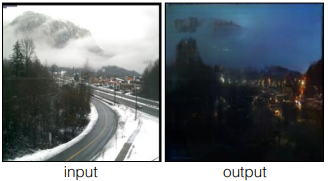
\includegraphics[width=0.4\textwidth]{img/model0.png}
    \caption{Realistic image colorization}
    \subcaption*{\textit{source: \textcolor{blue}{https://arxiv.org/pdf/1611.07004v1.pdf}}}
    \label{fig:Model-0}
  \end{figure}
    \section{Manga Colorization Using Reference Images\cite{qu2006manga}}
    Colourizing manga by tracing pattern continuity and intensity continuity.
	Intensity continuity to avoid colour bleeding. This is manual and proper edge detection is not possible with the pattern continuity method.
    \begin{figure}[htbp]
    \centering
    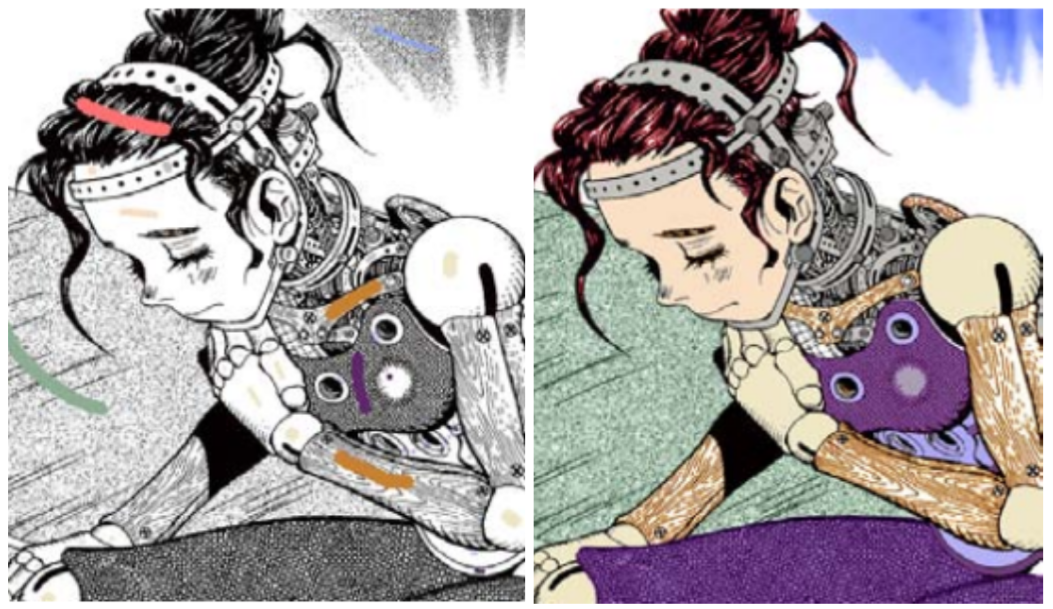
\includegraphics[width=0.4\textwidth]{img/model1.png}
    \caption{Colorization using pattern continuity}
    \subcaption*{\textit{source: \textcolor{blue}{https://www.youtube.com/watch?v=HpZUOq3O64s}}}
    \label{fig:Model-1}
  \end{figure}
    \newpage
    \section{cGAN-based Manga Colorization Using a Single Training Image\cite{hensman2017cganbased}}
    They used cGAN based approach for colorization along with segmentation of manga to produce high resolution and clean images.This method fails to generalise colorization for diverse characters and suffers heavily from colour monotonicity. 
    \begin{figure}[htbp]
        \centering
        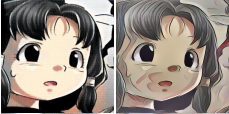
\includegraphics[width=0.6\textwidth]{img/model2.png}
        \caption{Colorization using single image reference}
        \subcaption*{\textit{source: \textcolor{blue}{https://arxiv.org/pdf/1706.06918.pdf}}}
        \label{fig:Model-2}
      \end{figure}

    \section{Style Transfer for Anime Sketches with Enhanced Residual U-net and Auxiliary Classifier GAN\cite{ACPR2017ZLM}}
    Style maps and colour hints must be provided by the user for this network to perform colorization. Also the pretrained VGG is used which performs best for classification, but not for paintings.
    \begin{figure}[htbp]
        \centering
        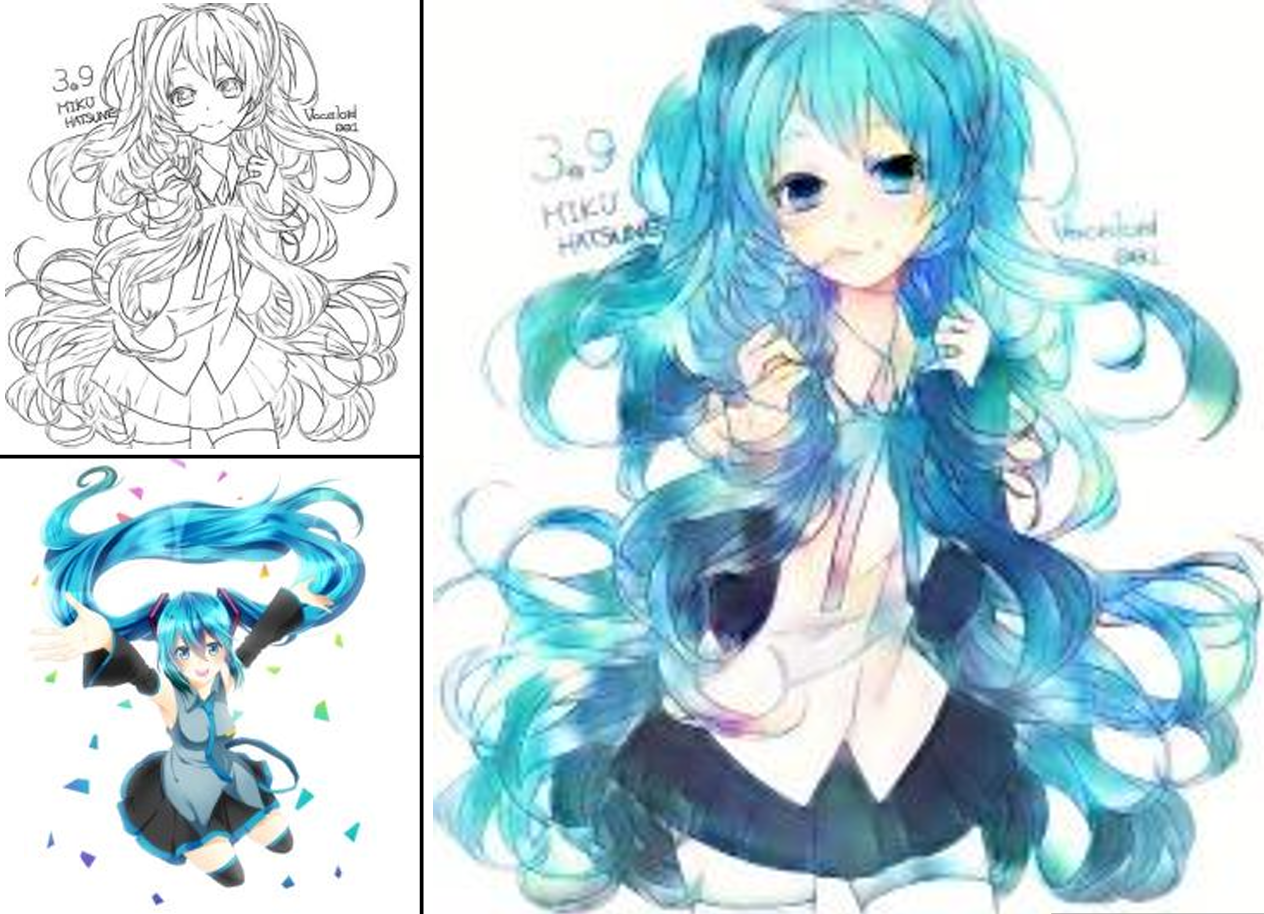
\includegraphics[width=0.6\textwidth]{img/model3.png}
        \caption{Colorization using style transfer method.}
        \subcaption*{\textit{source: \textcolor{blue}{https://arxiv.org/pdf/1706.03319.pdf}}}
        \label{fig:Model-3}
      \end{figure}
\newpage
    \section{inkn’hue: Enhancing Manga Colorization from Multiple Priors with Alignment Multi-Encoder VAE and StyleGAN\cite{jiramahapokee2023inkn}}
    Failed to fully automate the colorization process as a colour hints and partially coloured image was required as input for custom post processing.
    \begin{figure}[htbp]
        \centering
        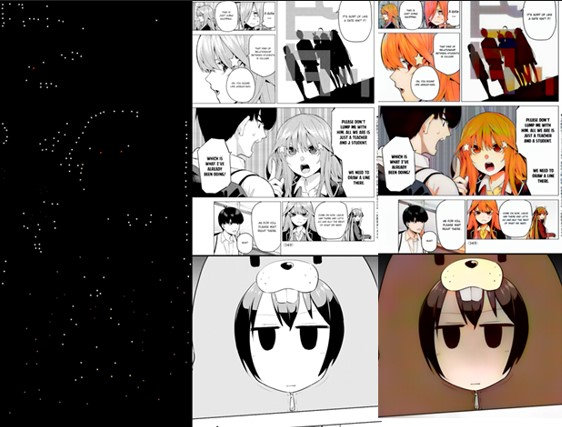
\includegraphics[height=0.4\textwidth]{img/model4.jpg}
        \caption{Semi-automatic colorization using multi-encoder VAE and StyleGAN}
        \subcaption*{\textit{source: \textcolor{blue}{https://arxiv.org/pdf/2311.01804.pdf}}}
        \label{fig:Model-4}
      \end{figure}
     \section{Semi-automatic Manga Colorization Using Conditional Adversarial Networks\cite{10.1007/978-3-030-72610-2_17}}
    If some object has several suitable colours, the neural network will produce a value
    close to the average of these colours that leads to degradation of the results, and monotone. 
    \begin{figure}[htbp]
        \centering
        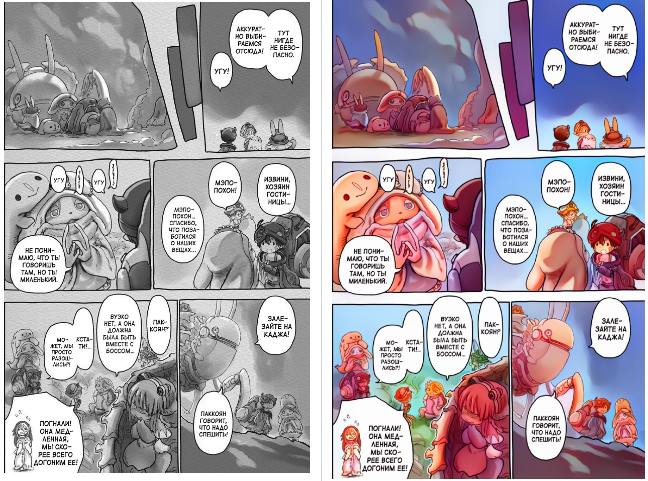
\includegraphics[width=0.5\textwidth]{img/model5.png}
        \caption{Semi-automatic colorization using cGAN}
        \subcaption*{\textit{source: \textcolor{blue}{https://github.com/qweasdd/manga-colorization-v2}}}
        \label{fig:Model-5}
      
      \end{figure}

\newpage
\section{Review Matrix}
\begin{table}[htp]
  \begin{tabular}{|c|p{4cm}|p{3cm}|p{4.5cm}|}
    \hline
    \textbf{S.N.} & \textbf{Title} & \textbf{Author(s)} & \textbf{Findings} \\ \hline
    
    1 & 
    Semi-automatic Manga Colorization Using Conditional Adversarial Networks \cite{10.1007/978-3-030-72610-2_17}  & 
    Maksim Golyadkin and Ilya Makarov &
    
    A cGAN-powntinuities, allowing users to personalize results with color hints and fine-tune for stylistic accuracy. \\ \hline

    2 & 
    Image-to-Image Translation with Conditional Adversarial Networks \cite{isola2018imagetoimage} & 
    Phillip Isola, Jun-Yan Zhu, Tinghui Zhou, and Alexei A. Efros & 
    This paper introduces cGAN for image-to-image translation, enabling the generation of realistic images by conditioning on input images from different domains. \\ \hline

    3 & 
    cGAN-based Manga Colorization Using a Single Training Image \cite{hensman2017cganbased} & 
    Kiyoharu Aizawa and Paulina Hensman &
    This method uses GANs to color entire manga pages, learning patterns and letting us personalize with hints and style tweaks. \\ \hline

    4 & Deep Extraction of x`Manga Structural Lines \cite{li-2017-deep} & Chengze Li, Xueting Liu, And Tien-Tsin Wong
    & It is a data-driven approach that uses CNN to identify structural lines in pattern-rich manga. \\ \hline

     5 & Style Transfer for Anime Sketches
    with Enhanced Residual U-net and Auxiliary Classifier GAN \cite{ACPR2017ZLM} &
    Lvmin Zhang, Yi Ji and Xin Lin & a method to apply the style of a painting to an anime sketch. \\ \hline

         \end{tabular}
\end{table}

\newpage

\begin{table}[htbp]
\centering
  \begin{tabular}{|c|p{4cm}|p{3cm}|p{4.5cm}|}
    \hline  
 
    6 & 
    Comicolorization: Semi-Automatic Manga Colorization \cite{furusawa2017comicolorization} & 
    Chie Furusawa, Kazuyuki Hiroshiba, Keisuke Ogaki and Yuri Odagiri & 
    This paper semi-automatically colorizes monochrome manga images using reference images, maintaining consistent colors for characters across panels, and allows for user revisions. 
    \\ \hline
  

    7 & Deep Residual Learning for Image Recognition \cite{he2015deep} & Kaiming He, Xiangyu Zhang, Shaoqing Ren, and Jian Sun & 
     This approach to convolution solves gradient vanishing problem allowing us to train very deep networks. 
     \\ \hline

    8 & U-Net: Convolutional Networks for Biomedical Image Segmentation \cite{ronneberger2015unet} & Olaf Ronneberger, Philipp Fischer, and Thomas Brox &
     Encoder and decoder architecture of U-net can be used for obtaining high resolution output and also enables 
     better image segmentation.
     \\ \hline

    9 & A Style-aware Discriminator for Controllable Image Translation \cite{kim2022styleaware} & Kunhee Kim, Sanghun Park, Eunyeong Jeon, Taehun Kim, and Daijin Kim &  
    The paper proposes a style-aware discriminator that acts as a critic and a style encoder to provide conditions which learns a controllable style space using prototype-based self-supervised learning and guides the generator.\cite{kim2022styleaware}
    \\ \hline

    10 & Wasserstein GAN \cite{arjovsky2017wasserstein} & Martin Arjovsky, Soumith Chintala, and Léon Bottou & This paper aims to solve mode collapse and hyperparameter sensitivity present in GANs using Wasserstein distance. 
    \\ \hline

    11 & Unpaired Image-to-Image Translation using Cycle-Consistent Adversarial Networks
    \cite{zhu2020unpaired} &
    Jun-Yan Zhu, Taesung Park, Phillip Isola, Alexei A. Efros & Style transfer between two sets of unpaired image dataset is possible. 
    \\ \hline
    
 \end {tabular}
  \caption{ Review Matrix with Research Papers, Authors, and Findings.}
  \label{tab:literature}
\end{table}

    \pagenumbering{arabic}
\setcounter{page}{9}
\chapter{Analysis}

\section{Requirement Analysis}
\subsection{Hardware Requirements}
\begin{itemize}
    \item   High capacity \textbf{RAM} to handle memory-intensive tasks
    \item   \textbf{Nvidia RTX series GPU} for CUDA based computations
    \item   \textbf{SSD storage} for faster read/write speeds during image processing
    \item   Additional high-capacity \textbf{external storage} for storing large datasets and image collections
\end{itemize}

\subsection{Software Requirements}
\begin{itemize}
    \item \textbf{Python3.10} - a high-level, general-purpose programming language.
    \item \textbf{Torch} - an open source ML library used for creating deep neural networks and is written in the Lua scripting language.
    \item \textbf{Torchvision} - a library consisting of popular datasets, model architectures, and image transformations for computer vision.
    \item  \textbf{FastAPI} - a modern web framework for building RESTful APIs in Python.
    \item \textbf{HTML/CSS/Javascript} - set of languages used for creating web pages
    \item  \textbf{SSH/RDP} - network communication protocols to access the remote server for development purposes.
    \item  \textbf{VSCode} - code editor for development.
    \item  \textbf{Git/GitHub} - version control System and repository.
    \item \textbf{Ngrok} - a tool that creates a secure tunnel to the localhost
    \item \textbf{Tensorflow} - a machine learning framework for building and training neural networks.
    \item \textbf{Keras} - a high-level neural networks API running on top of TensorFlow that facilitates fast experimentation and prototyping.
    \item \textbf{Visdom} - a Python library for creating interactive visualizations and monitoring the training of machine learning model.
\end{itemize}
\pagebreak

\section{Feasibility Study}
\subsection{Economic Feasibility}
    The total expenditure of the project is just computational power. For this, the college has assisted us with a remotely accessible virtual machine that is sufficiently capable for our project.  As for the other aspects of this project, none of them pose any economic cost. The process of acquisition and preparation of dataset required to train the model is explained in the methodology section.

\subsection{Techical Feasibility}
    The dataset, acquired in accordance with the Fair Usage Policy, will be preprocessed. This involves transforming the colored images into grayscale. Given the complexity of our model and the specifications of our machine, we anticipate a training duration of approximately 60 hours.

\subsection{Operational Feasibility}
    After the model is trained, a web interface will be created for user accessibility and interaction.  Furthermore, a Python package will also be created for easy integration into other codebases.

\subsection{Legal Feasibility}
    Manga are protected by copyright as works of art, making it difficult for large dataset for training. That’s why we have gathered legally available dataset to train our model under Fair Usage Policy.
    

    \pagenumbering{arabic}
\setcounter{page}{11}
\chapter{Methodology}
An iterative and incremental software development approach, such as Agile methodology, can be adopted. Agile methodologies emphasize flexibility, collaboration,
and iterative development, which align well with the nature of the project and its
potential changes and refinements.\\

\section{Agile Methodology}
Agile development is a flexible and iterative approach to software development that prioritizes adaptability and collaboration. It emphasizes delivering small, incremental releases of a product with the goal of responding quickly to changing requirements and feedback. Agile methodologies are based on the Agile Manifesto, which values individuals and interactions, working solutions, customer collaboration, and responding to change over rigid processes and tools.\\
\begin{figure}[H]
    \centering
    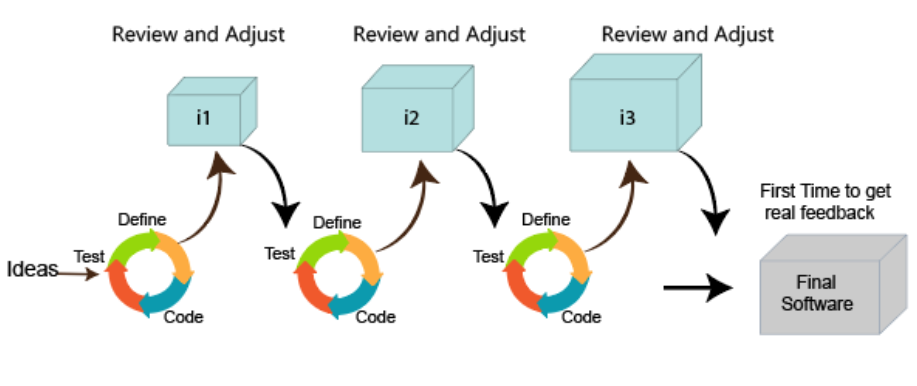
\includegraphics[width=1\textwidth]{img/agile.png}
    \caption{Agile methodology}
    \subcaption*{\textit{source: \textcolor{blue}{https://www.javatpoint.com/advantage-and-disadvantage-of-agile-methodology}}}
\end{figure}
The Agile development process is typically organized into iterations or sprints, each of which includes the following key steps:\\
\begin{itemize}

  \item \textbf{Requirements}:
        In Agile, requirements are expressed as user stories, which are short descriptions of a feature told from the perspective of the end user.
        Typically, the product owner collaborates with stakeholders to define and prioritize user stories, which in our case, are the objectives and highlights of the problem statement. These stories are added to the product backlog.

  \item \textbf{Design}:
        Design involves planning how the requirements will be implemented, considering the overall architecture, user interface, and other relevant aspects.
        During sprint planning, the development team discusses and plans how to address the problem statements and achieve the objectives. Design decisions are made collaboratively, and the team may create mockups or prototypes to visualize the solution.\\
  \item \textbf{Development}:
        This phase involves coding or implementing the solutions outlined in the design phase.
        Development work is carried out based on the tasks assigned to team members during the sprint planning. Continuous collaboration and communication are crucial to address any issues or changes that may arise.\\

  \item \textbf{Testing}:
        Testing is an integral part of Agile development and involves validating that the implemented features meet the specified requirements.
        Testing will be done parallely with development, creating test cases based on user stories and conducting various testing types (unit testing, integration testing, etc.) to ensure the quality of the code and output.\\

  \item \textbf{Deploy}:
        Deployment involves making the developed features available for use by end-users.
        The product increment is deployed to a staging or production environment. Continuous integration and deployment practices ensure that the latest changes are automatically integrated and deployed when ready.\\


  \item \textbf{Review}:
        At the end of each iteration, a review or demo is conducted to showcase the completed features to stakeholders.
        The team will participate in a review meeting to provide feedback, discuss any adjustments needed, and reprioritize the product backlog.\\

  \item \textbf{Launch}:
        The final step involves releasing the product increment to users. In our project, a web interface will be rolled at launch which will facilitate user interaction.
        Once all necessary adjustments are made based on feedback and the priorities based on objectives the product is officially launched. The cycle then repeats with a new iteration.\\
\end{itemize}

It's important to note that the design, development, testing, deployment, review, and launch steps occur iteratively and multiple times throughout the project. Agile development promotes continuous improvement and adaptation to changing requirements, allowing teams to deliver value to users more frequently and efficiently.\\



\pagebreak







    \chapter{System (or Project) Design and Architecture}
        % flowchart, description, Architecture

 

\section{Cycle-GAN}
\begin{figure}[htbp]
  \centering
  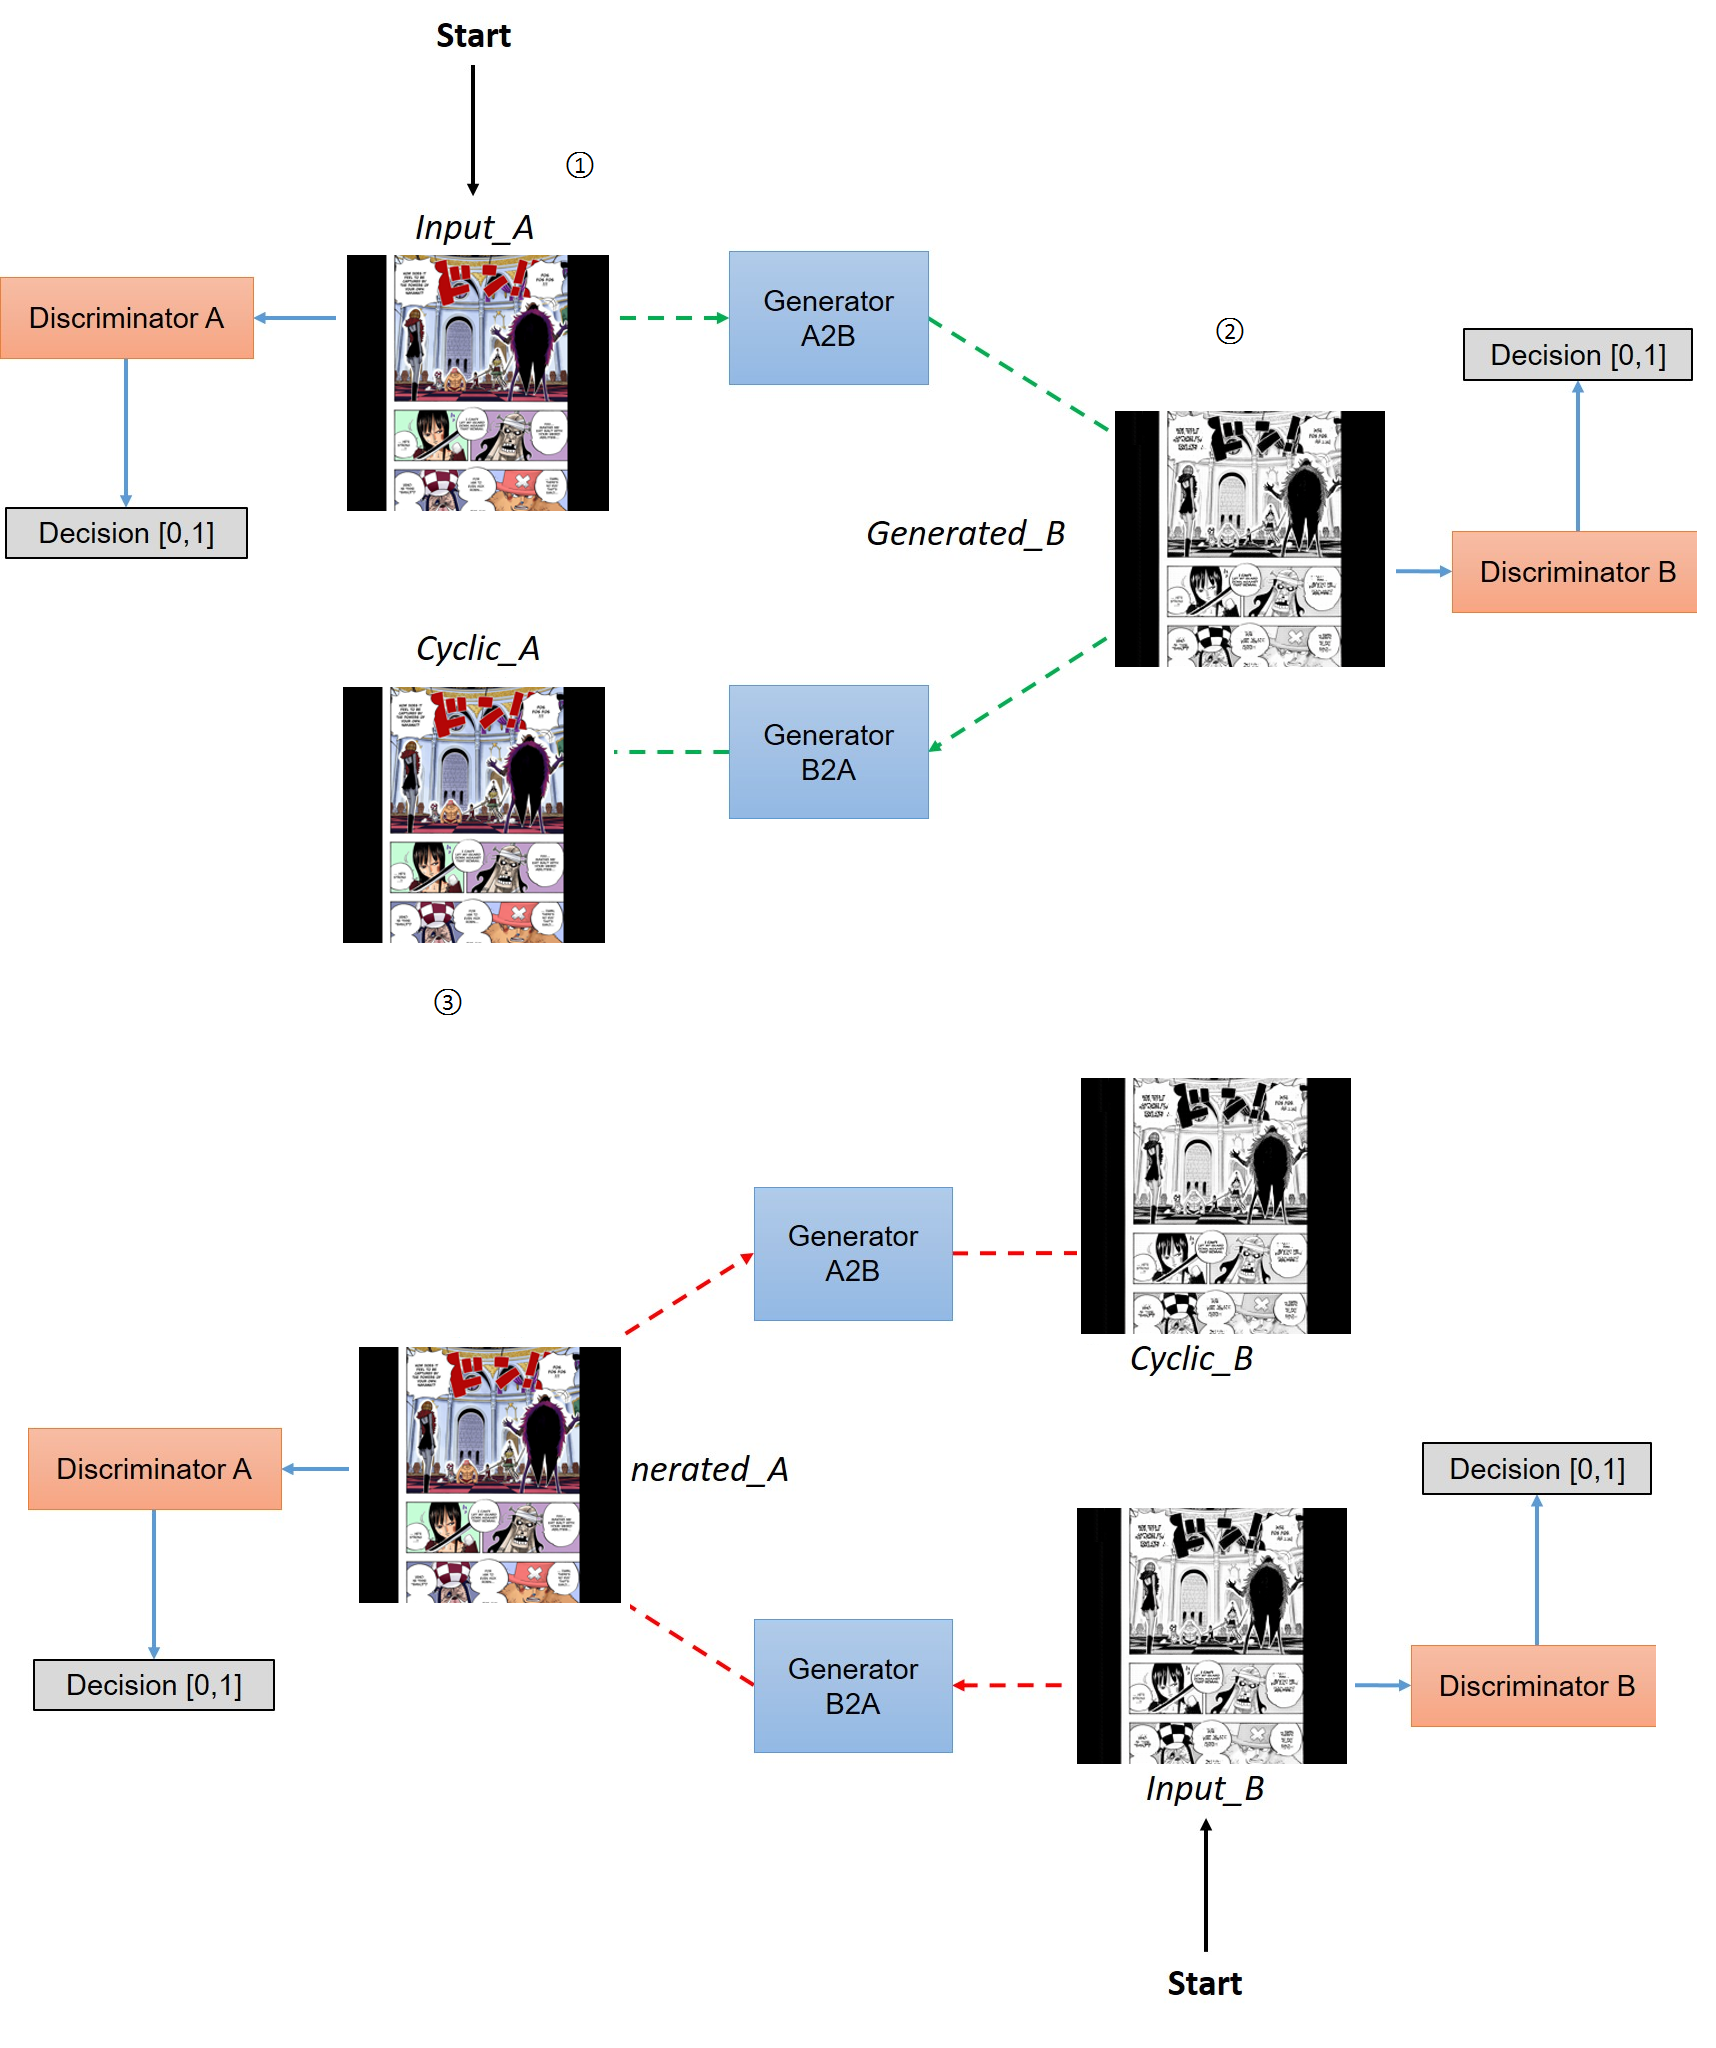
\includegraphics[width=0.8\textwidth]{img/GAN_block_diagram.png}
  \caption{Cycle-GAN implementation for manga colorization}
  \label{fig:cycle-gan-implementation}
\end{figure}
CycleGAN \cite{zhu2017unpaired} is a model proposed for performing image-to-image translations without paired data. The key idea behind CycleGAN is to learn mapping functions between two domains A and B such that the distribution of images from domain A mapped to domain B is similar to the distribution of images in domain B, and vice versa .
\pagebreak
CycleGAN consists of two GANs - G: A → B and F: Y → X. G tries to transform images from domain A to look like they came from domain B, and F does the opposite.

Along with the generators G and F, there are also two discriminators, DA and DB. DA tries to distinguish between images from domain A and generated images from F. Similarly, DB tries to distinguish between images from domain B and generated images from G. \cite{zhu2020unpaired}.
\\
       
\subsection{Generator}
The ResNet9 generator is a variant of the ResNet architecture adapted for use in generative adversarial networks (GANs) for image synthesis tasks. It employs deep residual blocks with skip connections to capture complex patterns in input noise, while normalization layers stabilize training. Activation functions introduce non-linearity, enabling the model to learn intricate mappings between noise and generated images.
The generator takes a black and white manga panel as input and learns to predict the corresponding colored version of the manga panel. The generator passes images through series of convolution layers with downsampling and upsampling to produce colored output. The generator architecture (figure \ref{fig:Generator Architecture}) is constructed as in \cite{simonyan2015deep}. 

\begin{figure}[h!]
  \centering
  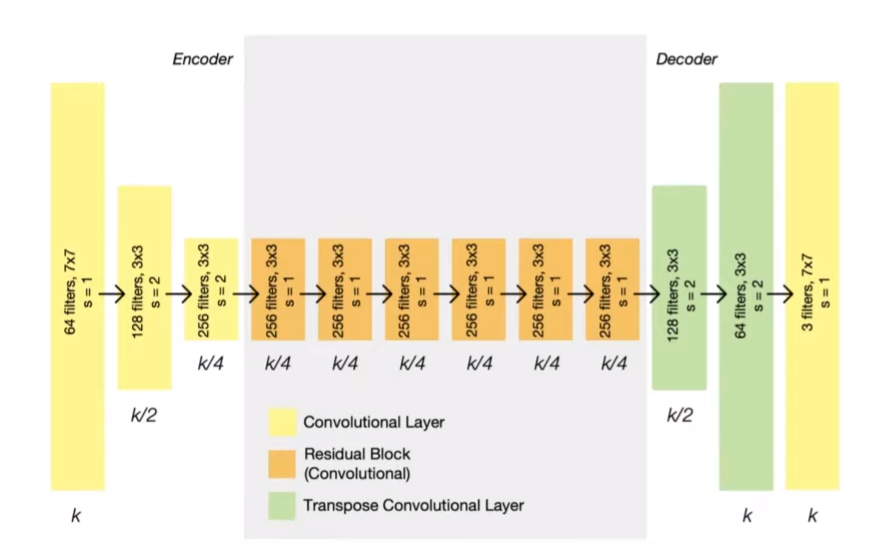
\includegraphics[width=0.8\textwidth]{img/generator (1).png}
  \caption{ResNet9 Generator Architecture }
  \label{fig:Generator Architecture}
\end{figure}

\subsection*{Input Processing}
The input image is initially processed through a series of layers to extract features. It starts with a reflection padding layer followed by a convolutional layer with a kernel size of 7 and 64 output channels.
Instance normalization is applied after the first convolutional layer, which normalizes the activations across the spatial dimensions of each channel independently for each sample in a batch.
\subsection*{Downsampling}
After the initial processing, the generator performs downsampling to reduce the spatial dimensions of the features while increasing the number of channels. This downsampling is achieved through two sets of convolutional layers with stride 2, effectively halving the spatial dimensions of the features while doubling the number of channels. Instance normalization and ReLU activation are applied after each downsampling operation.
\subsection*{Residual Blocks}
The core of the generator architecture consists of a series of residual blocks. These blocks aim to capture and refine image details across different scales. Each residual block contains two convolutional layers with 3x3 kernels, followed by instance normalization and ReLU activation. The input to each residual block is added to the output of the convolutional layers, allowing the network to learn residual mappings.
\subsection*{Upsampling}
After the residual blocks, the generator performs upsampling to reconstruct the high-resolution output image. Similar to the downsampling stage, upsampling is achieved through two sets of transposed convolutional layers. These layers increase the spatial dimensions while reducing the number of channels. Instance normalization and ReLU activation are applied after each upsampling operation.
\subsection*{Output Layer}
Finally, the upscaled features are passed through a reflection padding layer followed by a convolutional layer with a kernel size of 7 to generate the output image. The output image is normalized using the hyperbolic tangent (Tanh) activation function, which maps the pixel values to the range [-1, 1].

\begin{figure}[htbp]
    \centering
    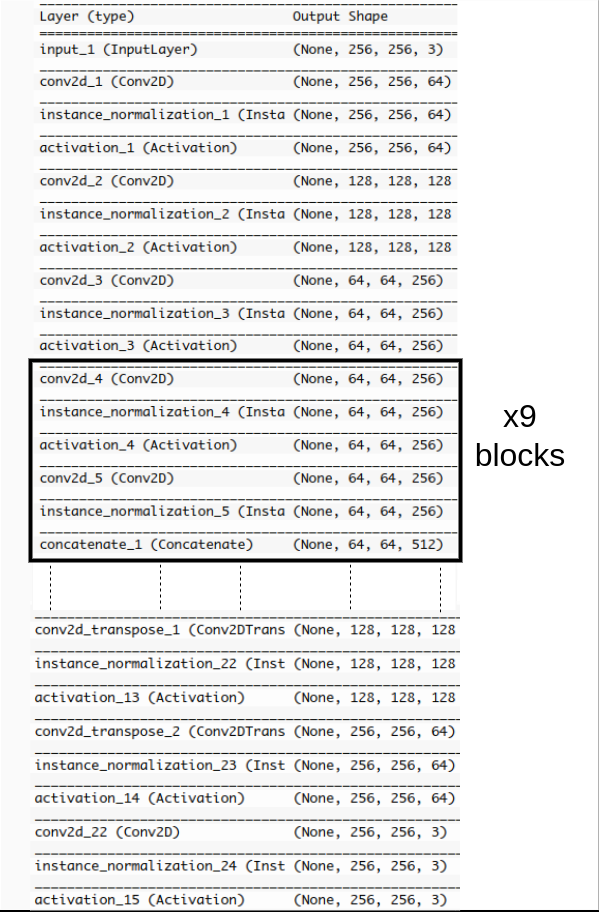
\includegraphics[width=0.8\textwidth]{chapter/output/gen_summary.png}
    \caption{Generator Architecture Summary}
    \label{fig:gen_summary}
\end{figure}

\pagebreak

\subsection{Discriminator}
The PatchGAN discriminator \cite{zhu2020unpaired} in CycleGAN is designed to discriminate between real and fake images at the patch level rather than the image level. It consists of convolutional layers with decreasing spatial dimensions and increasing channel depths.

\subsection*{Architecture}
The architecture follows a pattern of convolutional layers with increasing channel depths: C64-C128-C256-C512. Each layer is followed by a normalization step, often using instance normalization, and a non-linear activation function, typically Leaky ReLU.
\subsection*{Patch-Level Discrimination}
 Instead of outputting a single probability for the entire image, the discriminator outputs a matrix of probabilities corresponding to different patches of the input image. This patch-based approach allows the discriminator to capture fine-grained details and textures in both real and fake images.
 \subsection*{Final Layers}
 Although not mentioned in the paper \cite{zhu2020unpaired}, the discriminator includes a final hidden layer C512 with a stride of 1×1, followed by an output layer C1 also with a 1×1 stride, utilizing a linear activation function. This configuration enables the discriminator to produce an output feature map of size 16×16 when applied to an input image of size 256×256.
  \subsection*{Training Objective}
  The discriminator aims to minimize the classification error between real and fake patches, effectively learning to distinguish between authentic and generated image patches. \\
  
  By utilizing a PatchGAN discriminator, CycleGAN is able to enforce high-frequency structure consistency between input and output images, facilitating the translation of image style and domain adaptation tasks


%---------------------------------flowchart

\begin{figure}
  \centering
  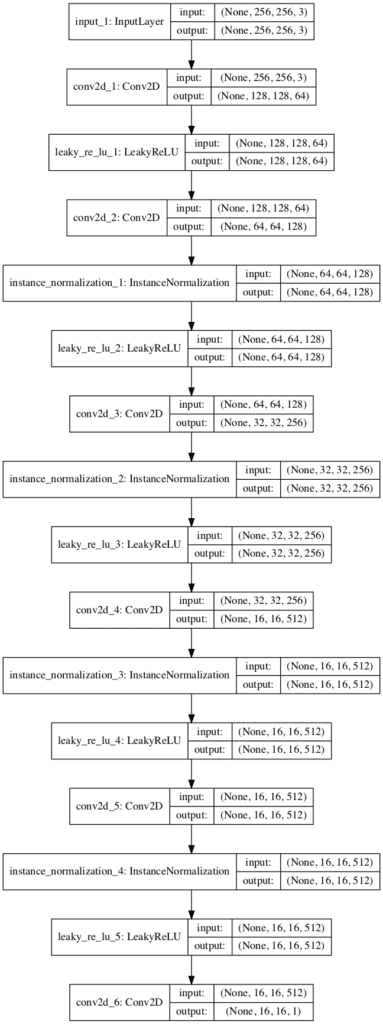
\includegraphics[height=1.25\textwidth]{img/discriminator_new.png}
  \caption{Discriminator Architecture }
  \label{Discriminator Architecture}
\end{figure}

\begin{figure}[p]
    \centering
    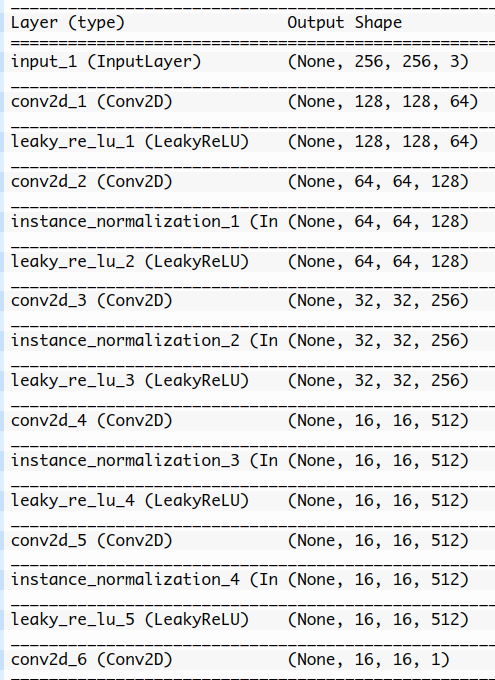
\includegraphics[width=1\textwidth]{chapter/output/disc_summary.png}
    \caption{Discriminator Architecture Summary}
    \label{fig:gen_summary}
\end{figure}




\newpage
\section{Loss Function}

To teach the model to generate similar colors for similar patterns and introduce a variety of colors, we use a mix of different loss functions.
\begin{itemize}
  \item \textbf{L1 Loss} \\
        In order to enforce the generator to produce similar coloring to the
        ground truth, we use a pixel level L1 metric that calculates the distance between
        output image $\mathcal{G}\left( x, d, h, \mathcal{E}\left( x \right)\right)$ and ground truth image y.
        \begin{equation}
          \mathcal{L}_{L_1}^\mathcal{G} = \|\mathcal{G}\left( x, d, h, \mathcal{E}\left( x \right)\right) - y \|
        \label{l1-loss}
        \end{equation}

        Where,
        \begin{itemize}
            \item $\mathcal{L}_{L_1}^\mathcal{G}$ = Generator L1 Loss
            \item $\mathcal{G}$ = Generator function
            \item x = Input to Generator
            \item d = Conditioning information
            \item h = Hidden state
            \item $\mathcal{E} (x)$ = Encoder function applied to input x
            \item y = Ground truth image
        \end{itemize}

  % \item \textbf{Perceptual Loss} \\
  %       To ensure similarity not only at the pixel level but also at the
  %       structural level, we use perceptual loss as described in \cite{10.1007/978-3-030-72610-2_17}. It’s an L2-loss based on
  %       the distance between some CNN feature maps for generated and ground truth
  %       images.

  %       \begin{equation}
  %         \mathcal{L}_{per}^\mathcal{G} = \frac{1}{chw}\| \mathcal{V} \left( \mathcal{G}\left( x, d, h, \mathcal{E}\left( x \right)\right)\right) - \mathcal{V}\left(y\right) \|
  %       \end{equation}
  %       Where, 
  %       \begin{itemize}
  %           \item $\mathcal{V}$ = a VGG-16 network
  %           \item c = number of channels
  %           \item h = height of feature maps
  %           \item w = width of feature maps
  %       \end{itemize}
      
  \item \textbf{Adversarial losses} \\
        For the mapping function G:X→Y and its discriminator D(y) , we express the objective as:
        \begin{equation}
          \mathcal{L}_\mathcal{G}{_{adv}}  =  \mathbb{E}_{x,h}[log\left( 1 - \mathcal{D} \left( \mathcal{G}_{main} \left( x, d \left( x \right), h, \mathcal{E} \left( x \right) \right) \right) \right)]
        \end{equation}
        where G tries to generate images G(x) that look similar to images from domain Y , while D(y) aims to distinguish between translated samples G(x) and real samples y. G aims to minimize this objective against an adversary D that tries to maximize it.

        We introduce a similar adversarial loss for the mapping
        function F : Y → X and its discriminator D(x) as well:
        \begin{equation}
          \mathcal{L}_D{_{adv}} = - \mathbb{E}_y [ log\mathcal{D}\left(y\right)] - \mathbb{E}_{x,h}[log\left(1 - \mathcal{D}\left(\mathcal{G}_{main}\left(x,d\left(x\right),h,\mathcal{E}\left(x\right)\right)\right)\right)]
        \end{equation}
        \pagebreak
  % \item \textbf{White Color Penalty Loss} \\
  %       We penalize the network if the pixel value is close to the maximum corresponding
  %       to the white color as found in \cite{10.1007/978-3-030-72610-2_17}. $\mathcal{L}_{white}$ is calculated as the mean square of the channel-wise
  %       sums (we assume that values of G output belong to [0, 1]).
  %       \begin{equation}
  %         \mathcal{L}_{white}^\mathcal{G} = \frac{\sum_{i,j,k}\left(white\_zones[i,j,k]\right)^2}{
  %           \sum_{i,j,k} mask[i,j,k] + 1
  %         }
  %       \end{equation}

  %       where,  $mask[i,j,k]$ is binary representation identifying the pixels in the color image exceeding a threshold of 0.85, and $white\_zones[i,j,k]$ represent the corresponding normalized bright regions in the genrated image.\\

  \item \textbf{Cycle Consistency Loss} \\
        Adversarial losses alone cannot guarantee that the learned function can map an individual input $x_i$ to a desired output $y_i$. To further reduce the space of possible mapping functions, the learned mapping functions should be cycle-consistent, for each image x from domain X, the image translation
        cycle should be able to bring x back to the original image,
        i.e., x → G(x) → F(G(x)) $\approx$ x. We encourage this behavior using a cycle consistency loss as found in \cite{zhu2020unpaired}:
        \begin{equation}
          \mathcal{L}_{cyc}\left(G,F\right) = \mathbb{E}_{x\sim p{_{data}}\left(x\right)}[\|F\left(G\left(x\right)\right) - x \|]
          + \mathbb{E}_{y\sim p{_{data}}\left(y\right)}[\|G\left(F\left(y\right)\right) - y\|]
        \end{equation}

        Where,
        \begin{itemize}
            \item $\mathcal{L}_{cyc}\left(G,F\right)$ = Cycle consistency loss between generators G and F
            \item $\mathbb{E}_{x\sim p{_{data}}\left(x\right)}$ = Expectation operator with respect to data distribution $p{_{data}}\left(x\right)$
            \item $\|.\|$ = Normalization operation
            \item $\mathbb{E}_{y\sim p{_{data}}\left(y\right)}$ = Expectation operator with respect to data distribution $p{_{data}}\left(y\right)$
            
        \end{itemize}

\end{itemize}

\section{Performance Evaluation Metrics}
Due to the architecture and domain similarity, we can use the same metrics as in \cite{huang2021fully} to evaluate the performance of our model.\\
\begin{itemize}
  \item \textbf{PSNR}: \\
       PSNR (Peak Signal-to-Noise Ratio) is a metric commonly used to measure the quality of reconstructed images or videos by comparing them to the original ones. It measures the ratio between the maximum possible power of a signal and the power of corrupting noise that affects the fidelity of its representation.

PSNR values are typically expressed in decibels (dB) and range from 0 to infinity. Higher PSNR values indicate higher image quality, with values closer to infinity representing perfect reconstruction.

In practical terms, PSNR values above 30 dB are often considered excellent, while values below 20 dB may indicate significant loss of quality.:
        \begin{equation}
          PSNR = 10 * log_{10}\left(\frac{MAX_I^2}{MSE}\right)l
        \end{equation}
        where, MAX  is the maximum possible pixel value of the image, (like 255 for 8-bit image). Mean Square Error (MSE) is an objective criterion between predicted images and real images, which is represents as:
        \begin{equation}
          MSE = \frac{1}{mn} \sum_{i=0}^{m-1} \sum_{j=0}^{n-1} \|T(i, j) - F(i, j)\|^2 l
        \end{equation}
        m , n represent the size of the real image and the colorized image respectively.\\

  \item \textbf{SSIM}:\\
        SSIM (Structural Similarity Index Measure) is a metric used to quantify the similarity between two images. It takes into account three components: luminance, contrast, and structure, to evaluate how closely the images resemble each other perceptually.

The SSIM values range from -1 to 1, where 1 indicates perfect similarity between the images, 0 indicates no similarity, and -1 indicates perfect dissimilarity. Typically, values above 0.9 are considered excellent, indicating high similarity between the images.
        \begin{equation}
          SSIM = \frac{(2\mu_x\mu_y + c_1)(\sigma_{xy} + c_2)}{(\mu_x^2 + \mu_y^2 + c_1)(\sigma_x^2 + \sigma_y^2 + c_2)}
        \end{equation}

        \begin{equation}
          c_1 = (k_1 L)^2 \quad c_2 = (k_2 L)^2
        \end{equation}
        where
        \begin{itemize}
          \item \( \mu_x \) is the mean of image x,
          \item \( \mu_y \) is the mean of image y,
          \item \( \sigma_x^2 \) is the variance of image x,
          \item \( \sigma_y^2 \) is the variance of image y,
          \item \( 	\sigma_{xy} 	\) is the covariance of image x and image y,
          \item L is dynamic range of pixel values, usually L is equal to 255,
          \item \( k_1 = 0.01\) and \( k_2 = 0.03\) which are constants for stability.
        \end{itemize}

\end{itemize} 
    \chapter{Experiments}


\section{Data Collection}
To train our CycleGAN model effectively, we collected a diverse dataset of manga images. We amassed a total of 53GB of data, consisting of 20GB of black and white images and 30GB of colored images in .cbz (Comic Book Zip) format. Each category comprised approximately 100 volumes, ensuring a balanced representation of both monochrome and colored styles.
To ensure consistent colorization results across our dataset and avoid issues arising from disparate artistic styles, we made the deliberate decision to utilize manga images exclusively from the series "One Piece" for training our Cycle-GAN model. \\
This choice was driven by several key factors:
\begin{itemize}
 \item \textbf{Uniform Art Style:}One Piece maintains a remarkable level of artistic consistency throughout its extensive volume count. This consistency provides the model with a well-defined framework for learning color palettes, shading techniques, and character depictions, ultimately leading to more faithful and visually unified colorization outputs.

\item \textbf{Data Abundance:} One Piece boasts a vast wealth of training data, encompassing hundreds of chapters across diverse settings, characters, and emotional portrayals. This abundance allows the model to acquire a comprehensive understanding of the series' overall color scheme and apply it effectively to unseen images.
\end{itemize}

However, it is crucial to acknowledge the potential limitations associated with this data selection:
\begin{itemize}
\item \textbf{Generalizability:}
Restricting the data to a single series may limit the model's ability to generalize effectively to other manga styles. Future exploration of transfer learning techniques could potentially address this limitation.
\item \textbf{Data Bias:} Utilizing solely One Piece introduces potential biases based on the specific color choices and techniques employed within that series. Diversifying the dataset in the future could help mitigate this issue.
\end{itemize}
\newpage

 

\section{Data Preprocessing}

To ensure the effectiveness of our CycleGAN model in colorizing manga images, we implemented a comprehensive data preprocessing pipeline specifically tailored to "One Piece" dataset. This process aimed to refine the raw dataset and provide the model with high-quality, consistent training material.

\subsection{CBZ Extraction and Conversion}

The initial step involved converting all collected CBZ files into individual PNG images. This conversion ensured compatibility with our Networks which accept images as inputs.

\subsection{Page Filtering}

For filtering at high level, we addressed the presence of RGB images in the dataset such as RGB cover pages, end pages, and special trivia and informative pages in the manga.

By effectively removing these colored pages, we ensured the model exclusively learned from black and white manga panels, preventing potential colorization inconsistencies arising from pre-colored content.

\subsection{Panel Detection and Classification}

Subsequently, we addressed the presence of non-manga pages \ref{fig:bad_images} within the dataset which typically are:
\begin{itemize}
    \item Empty pages
    \item Text-only or heavily text-biased pages
    \item Trivia and other non-manga-panel pages
\end{itemize}

To efficiently filter out these non-relevant pages, we employed a Sequential  Convolutional Neural Network (CNN) classifier featuring three 2D convolutional layers followed by max-pooling layers, then flattened and connected to two dense layers for classification. \\This classifier which has architecture as in figure \ref{fig:classifier} was trained on 69 bad manga panels and 900 good manga panels, with Precision: 0.9775, Recall: 1.0, Accuracy: 0.9797 on Validation data on 50 epochs of training.\\
With this CNN classifier, we could systematically identify and remove such non-manga pages from our dataset, ensuring that only relevant content was retained for further processing and analysis.

\begin{figure}[hp]
  \centering
  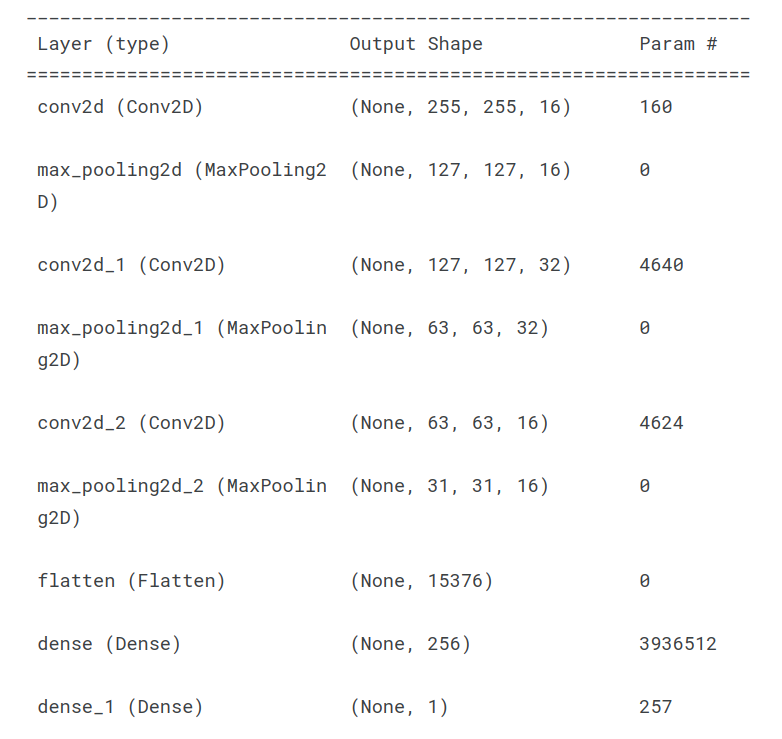
\includegraphics[width=1\textwidth]{chapter/output/classifier-summary.png}
  \caption{Architecture of Manga panel classifier}
  \label{fig:classifier}
\end{figure}


\begin{figure}[htbp]
    \centering
    \begin{subfigure}[b]{0.25\textwidth}
        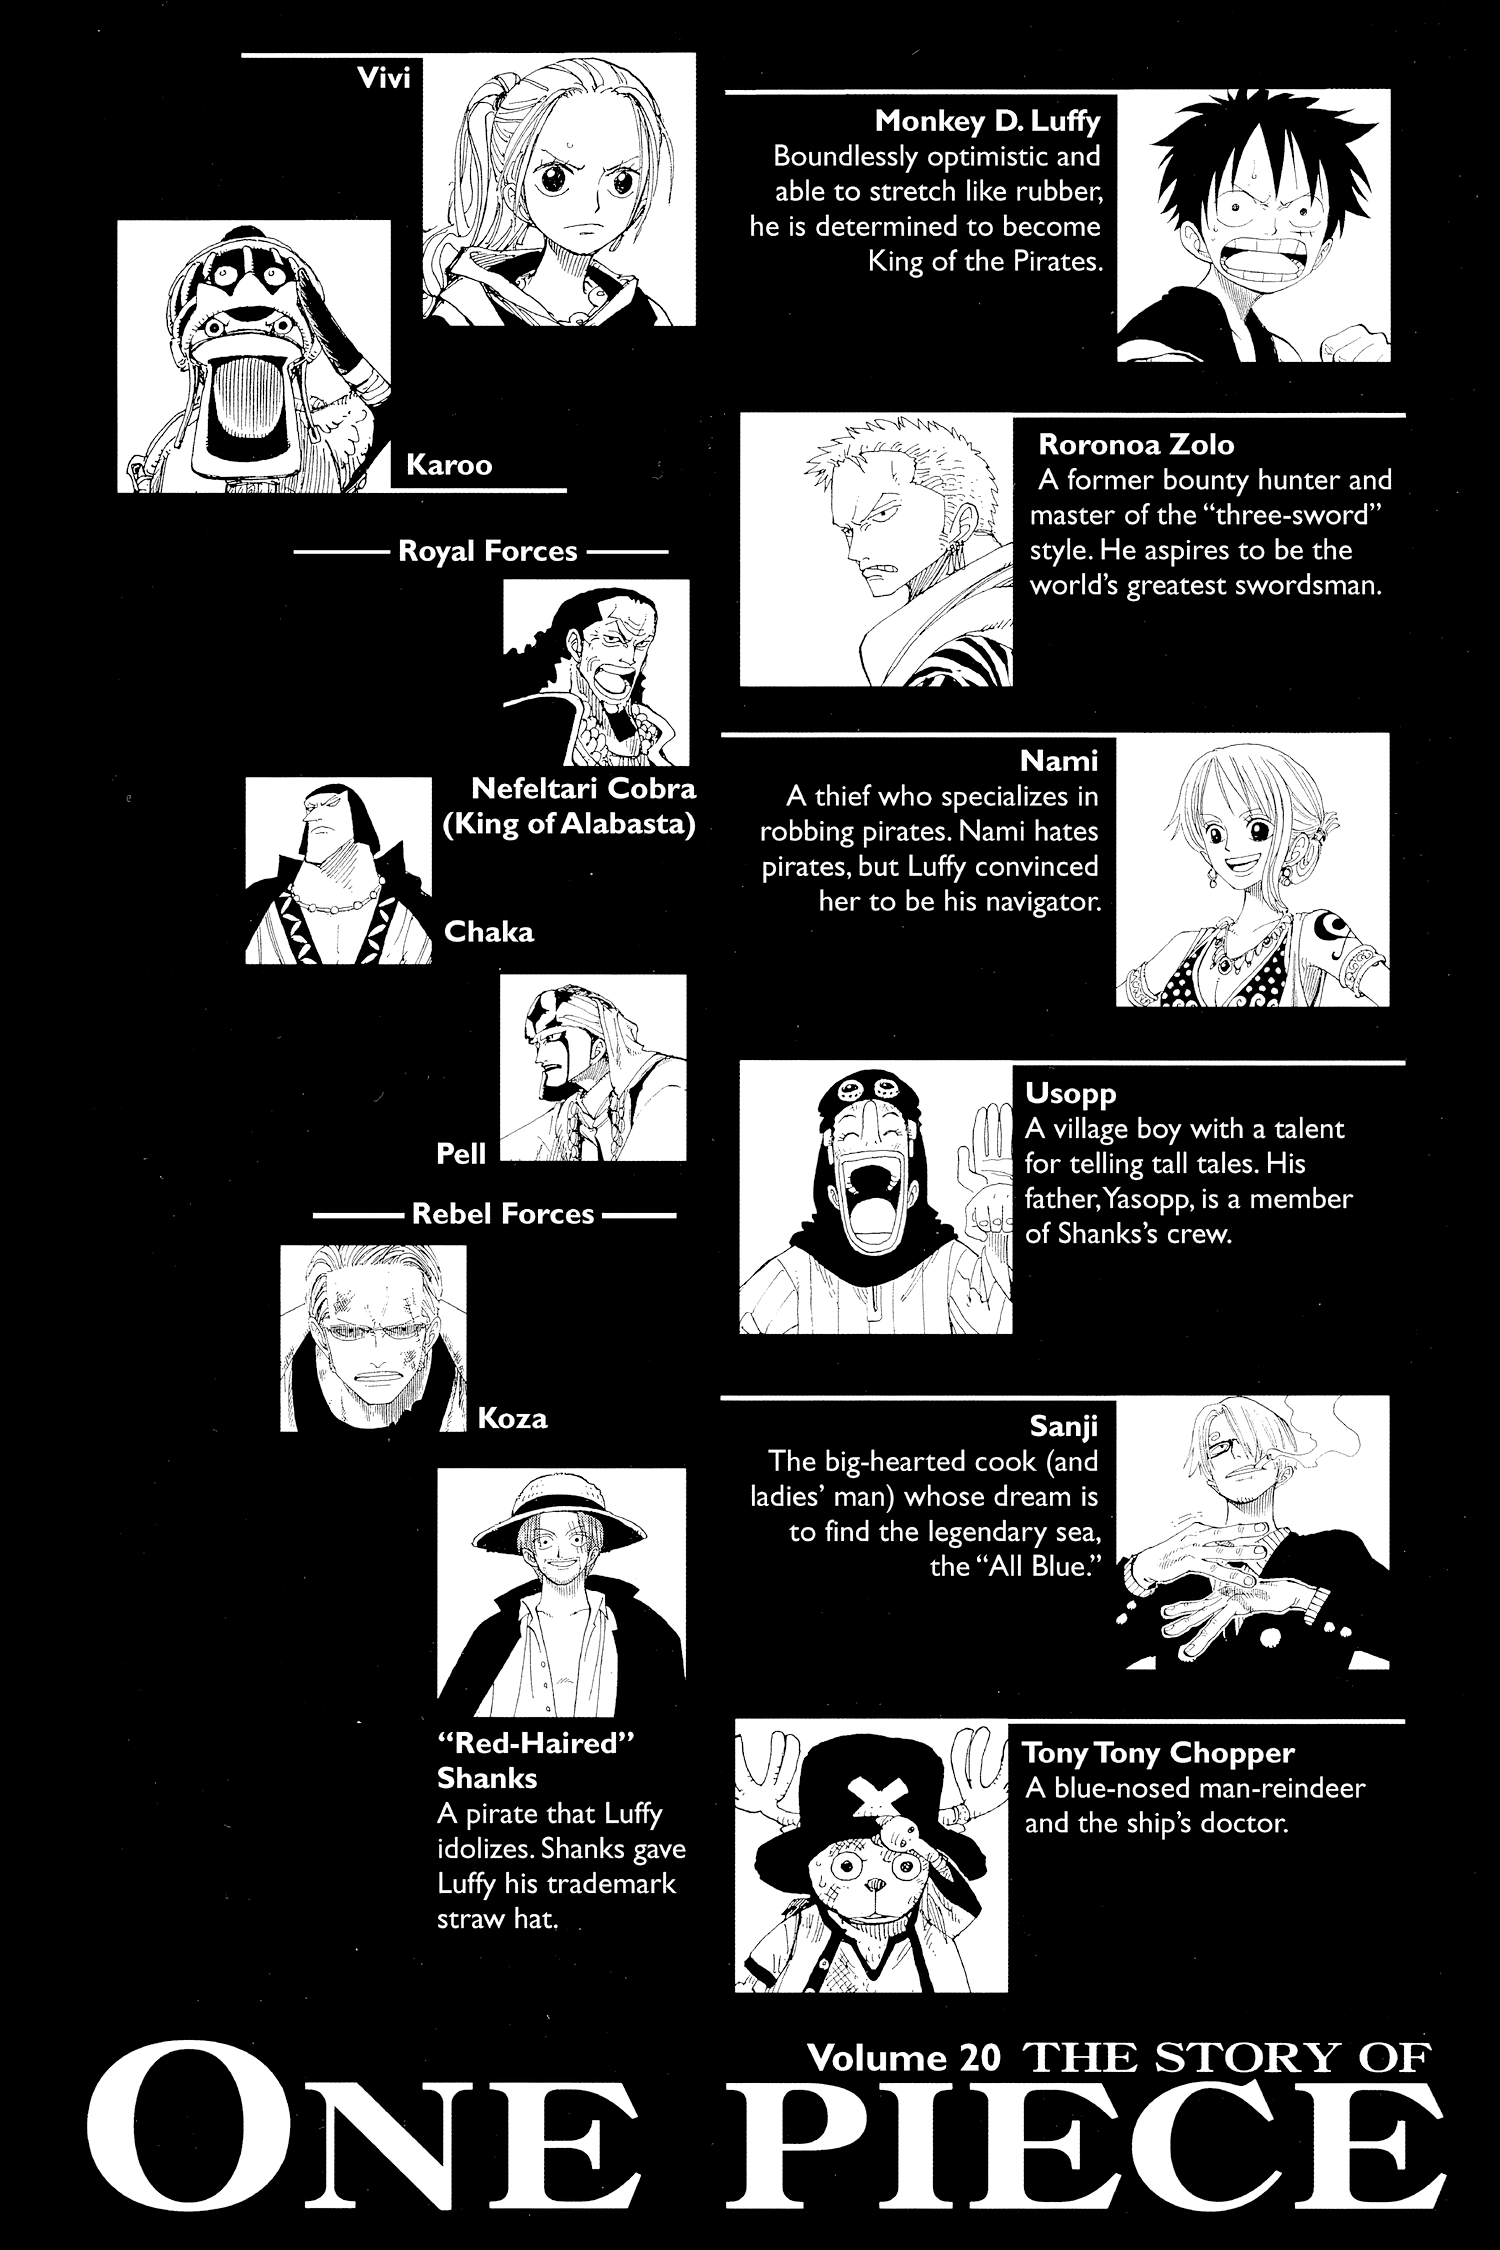
\includegraphics[width=\textwidth]{chapter/output/bad57.png}
      
    \end{subfigure}
    \hfill
    \begin{subfigure}[b]{0.25\textwidth}
        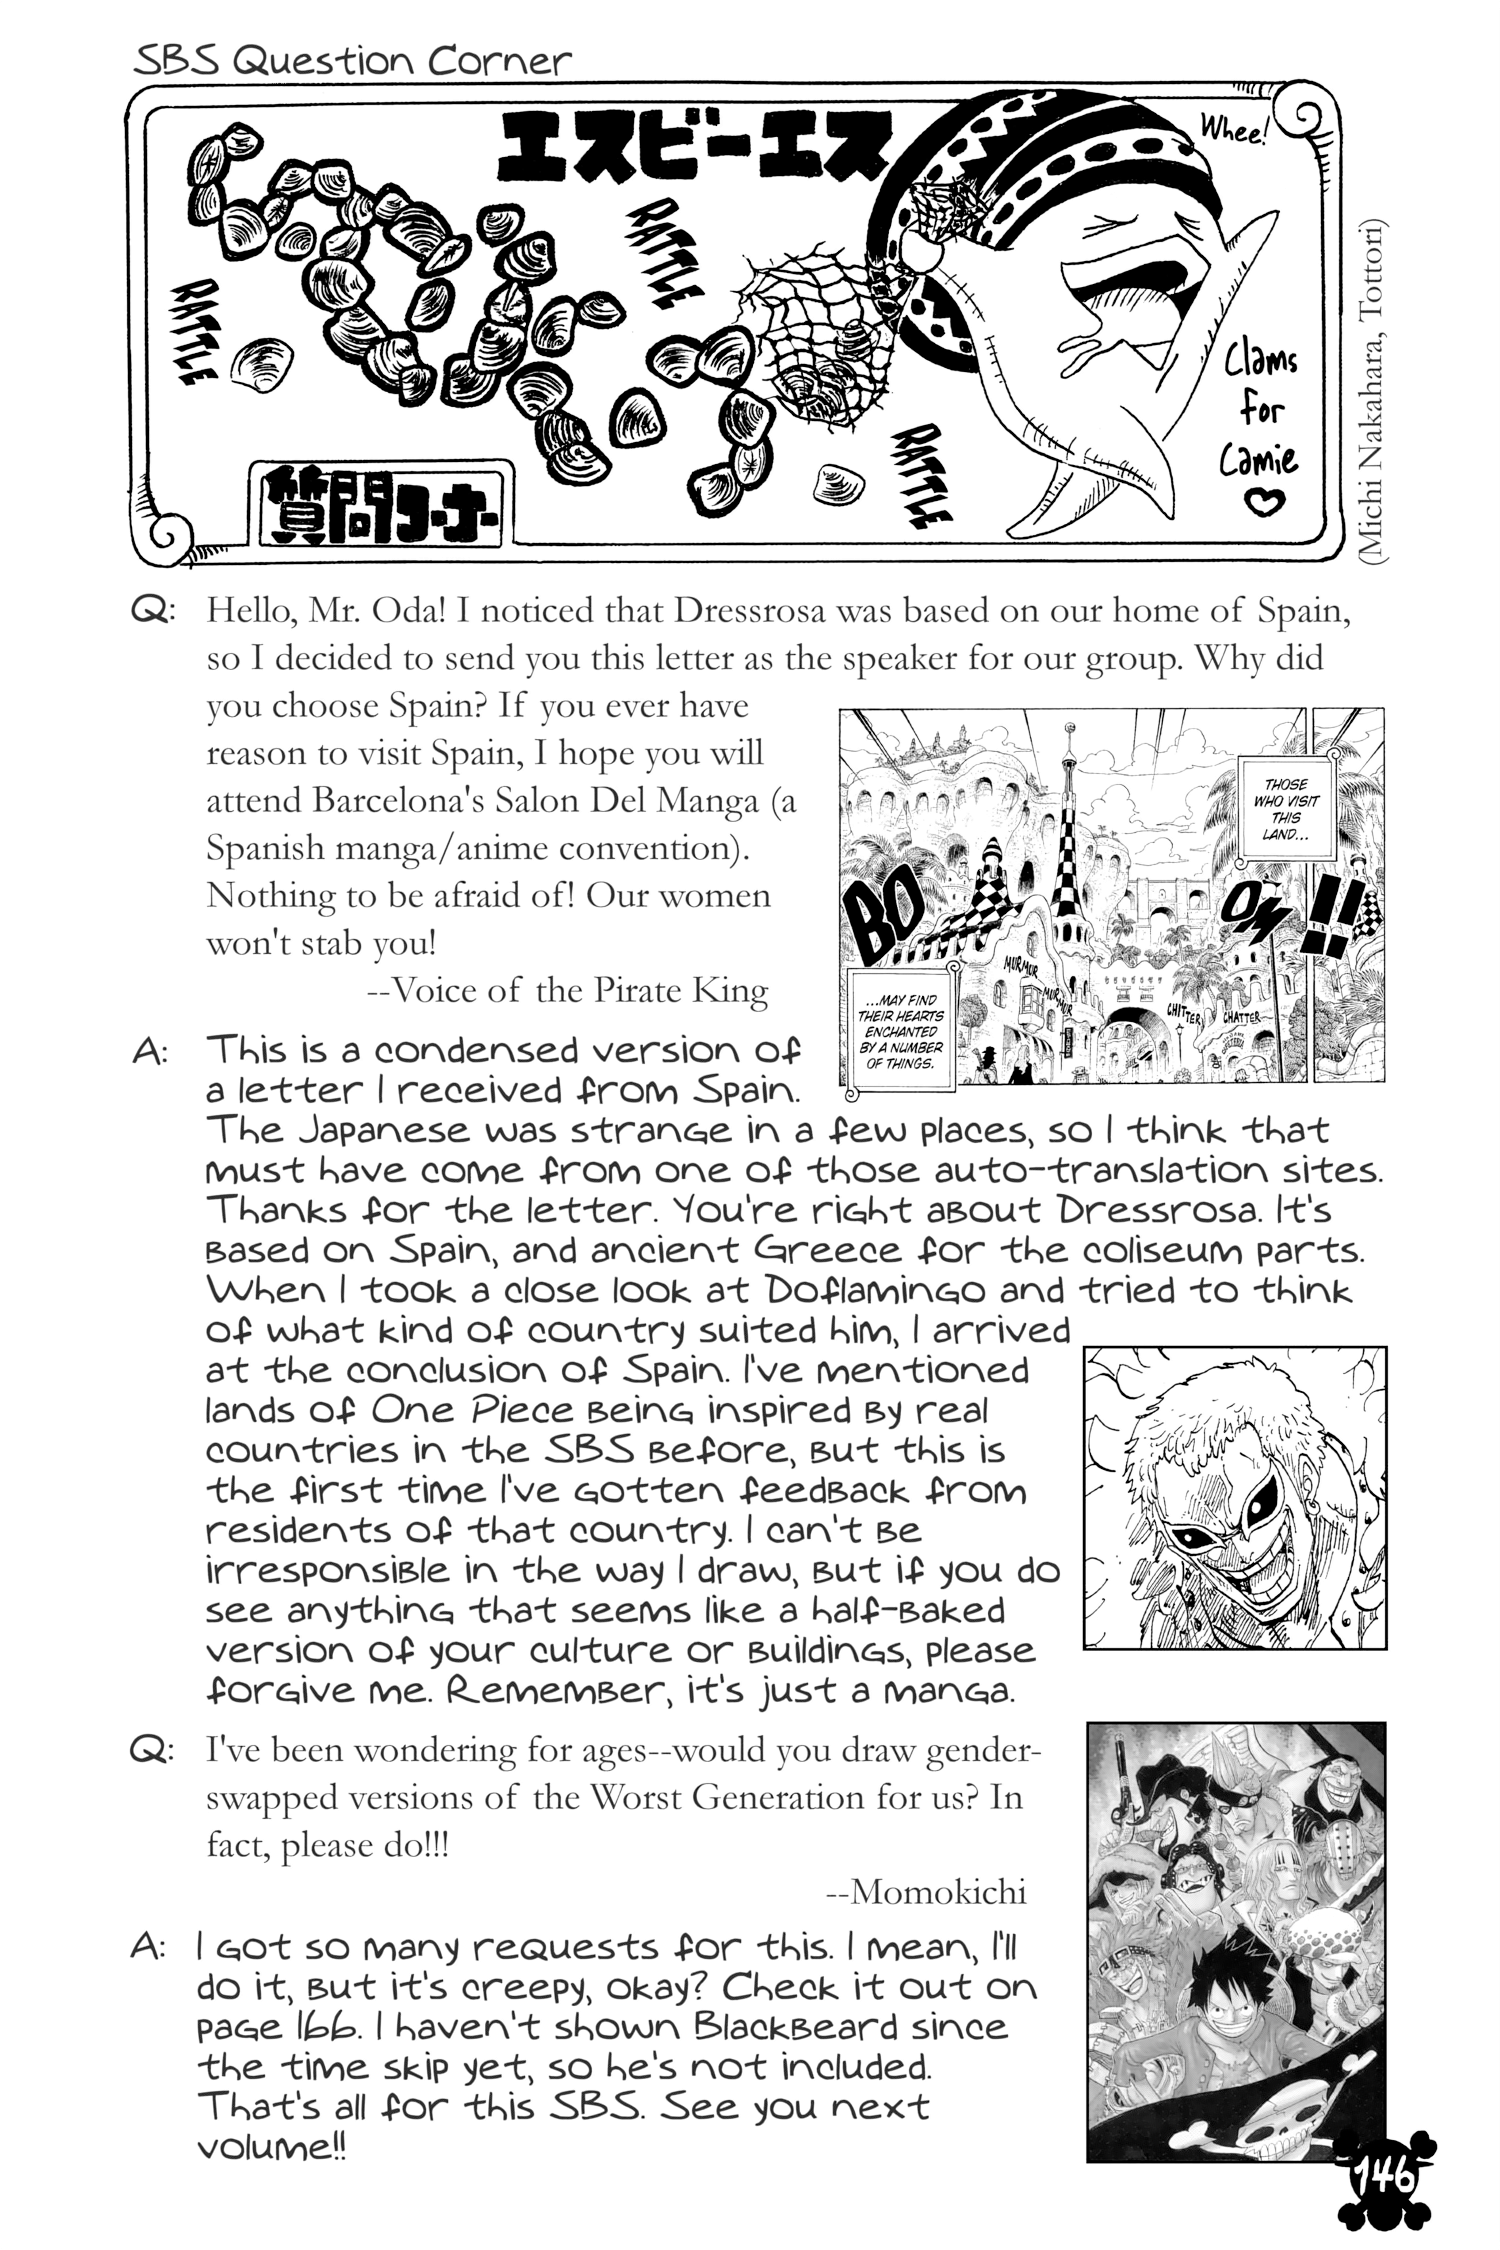
\includegraphics[width=\textwidth]{chapter/output/bw57.png}
        
    \end{subfigure}
    \hfill
    \begin{subfigure}[b]{0.2\textwidth}
        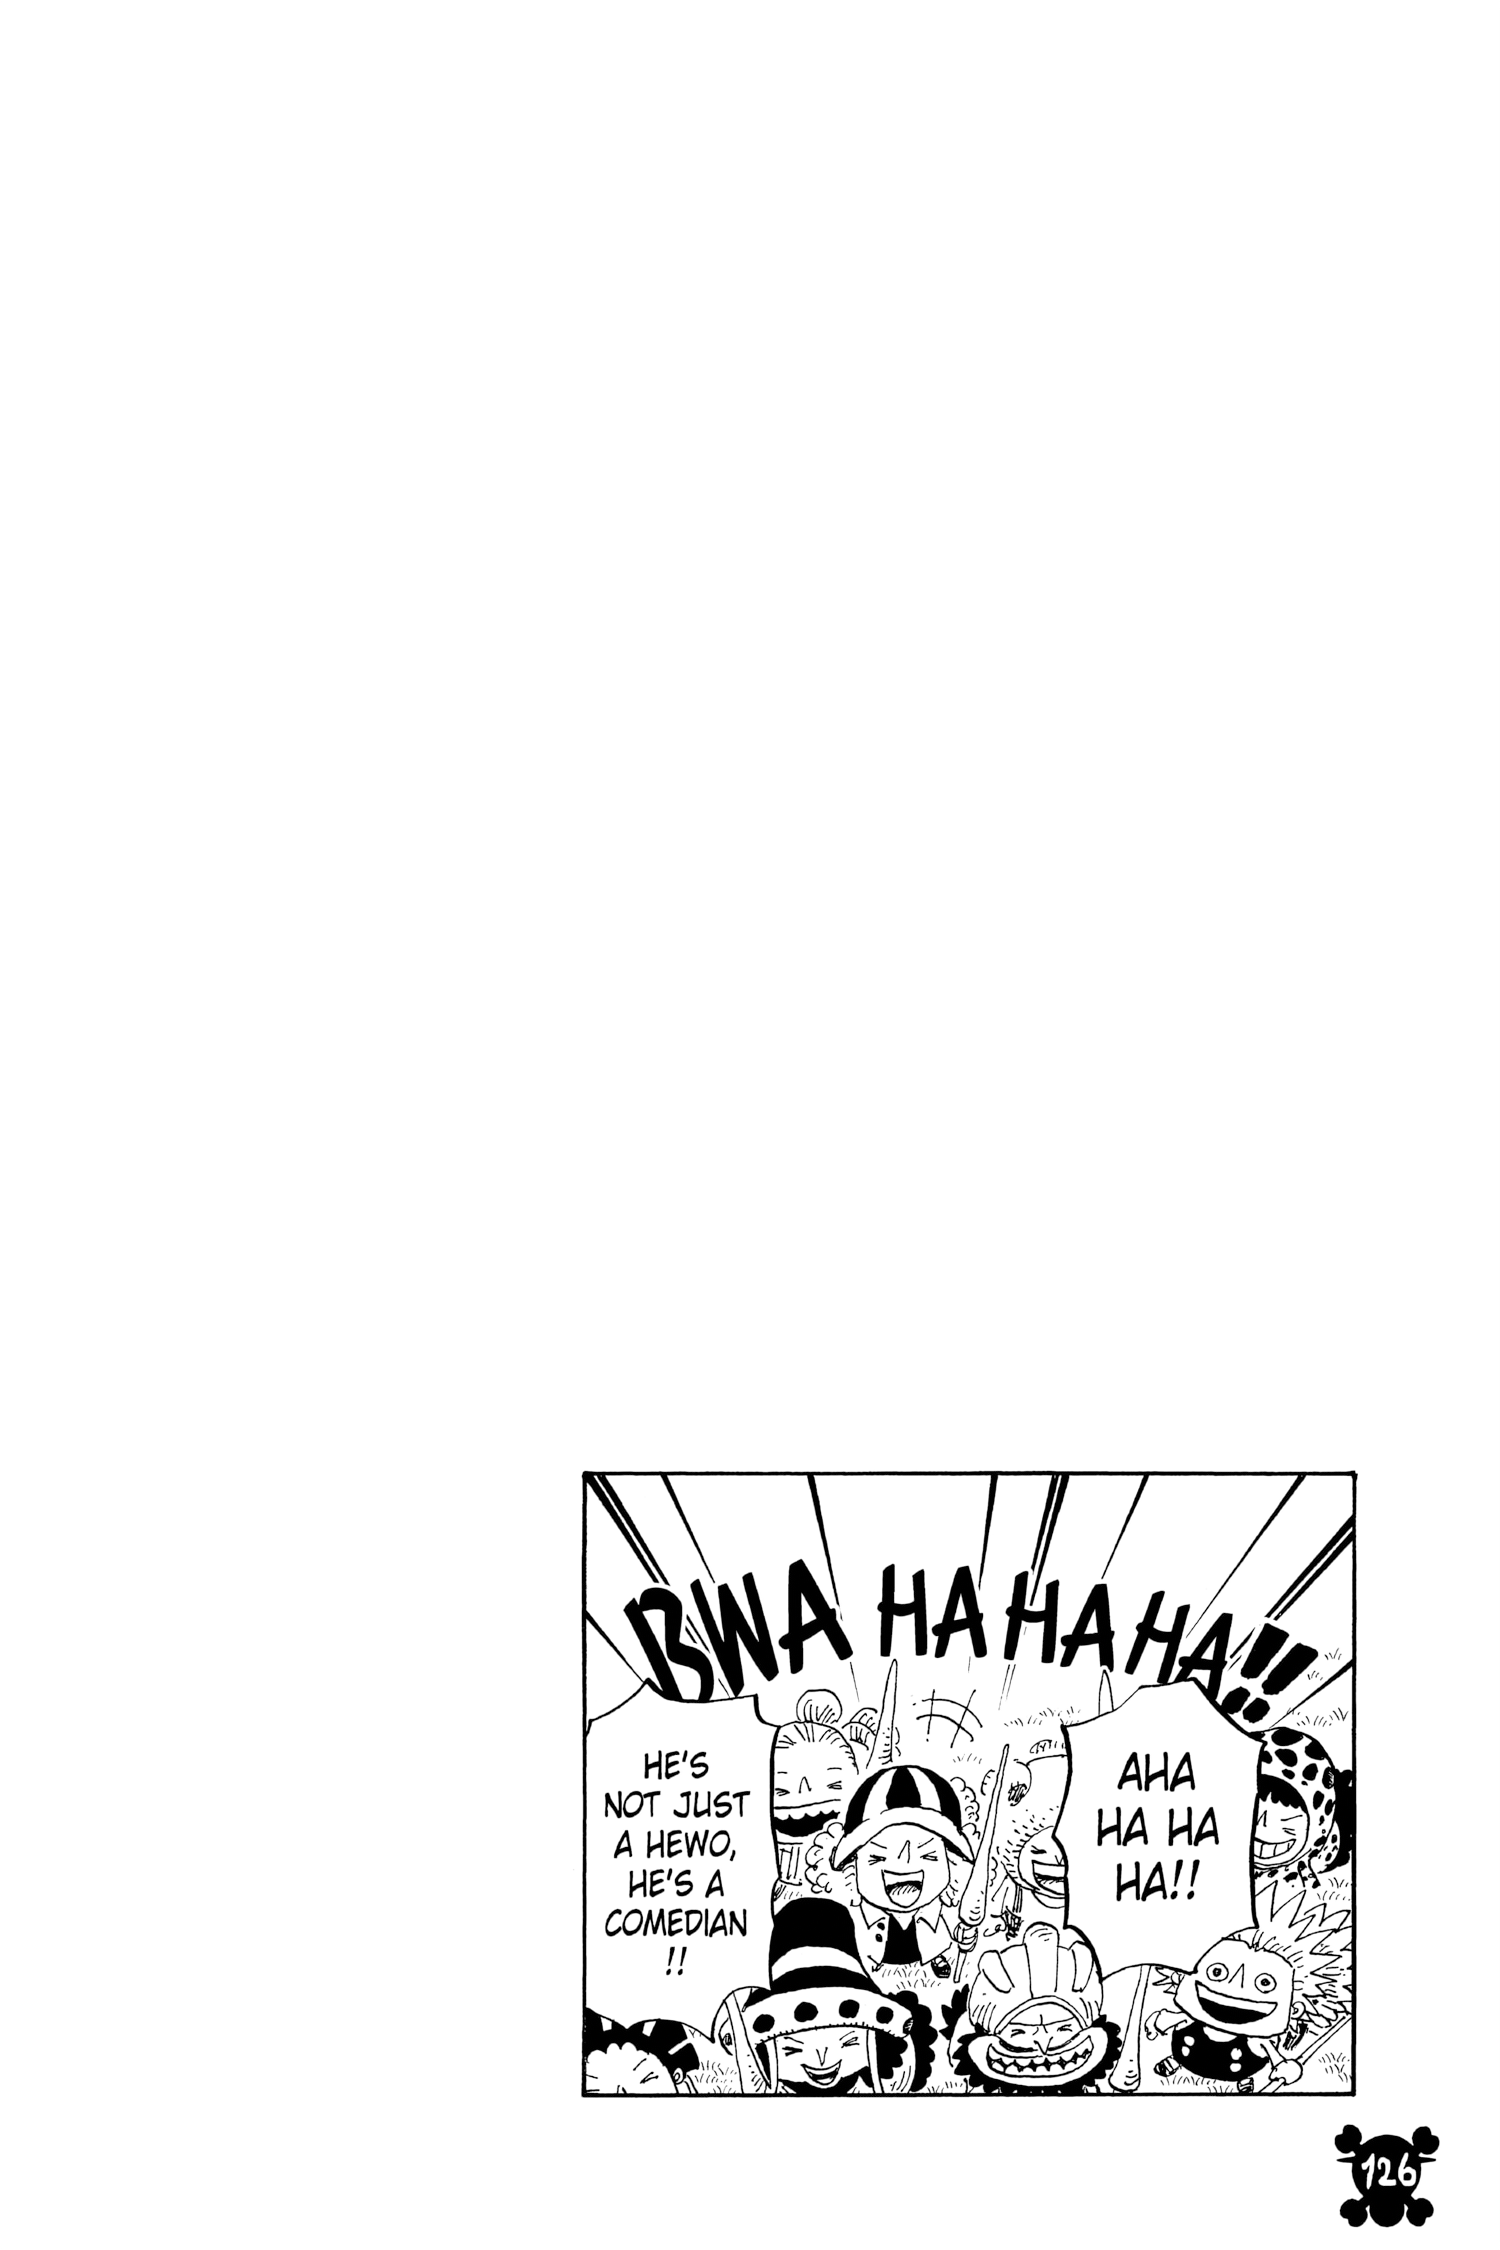
\includegraphics[width=\textwidth]{chapter/output/bw205.png}
       
    \end{subfigure}
    \hfill
    \begin{subfigure}[b]{0.25\textwidth}
        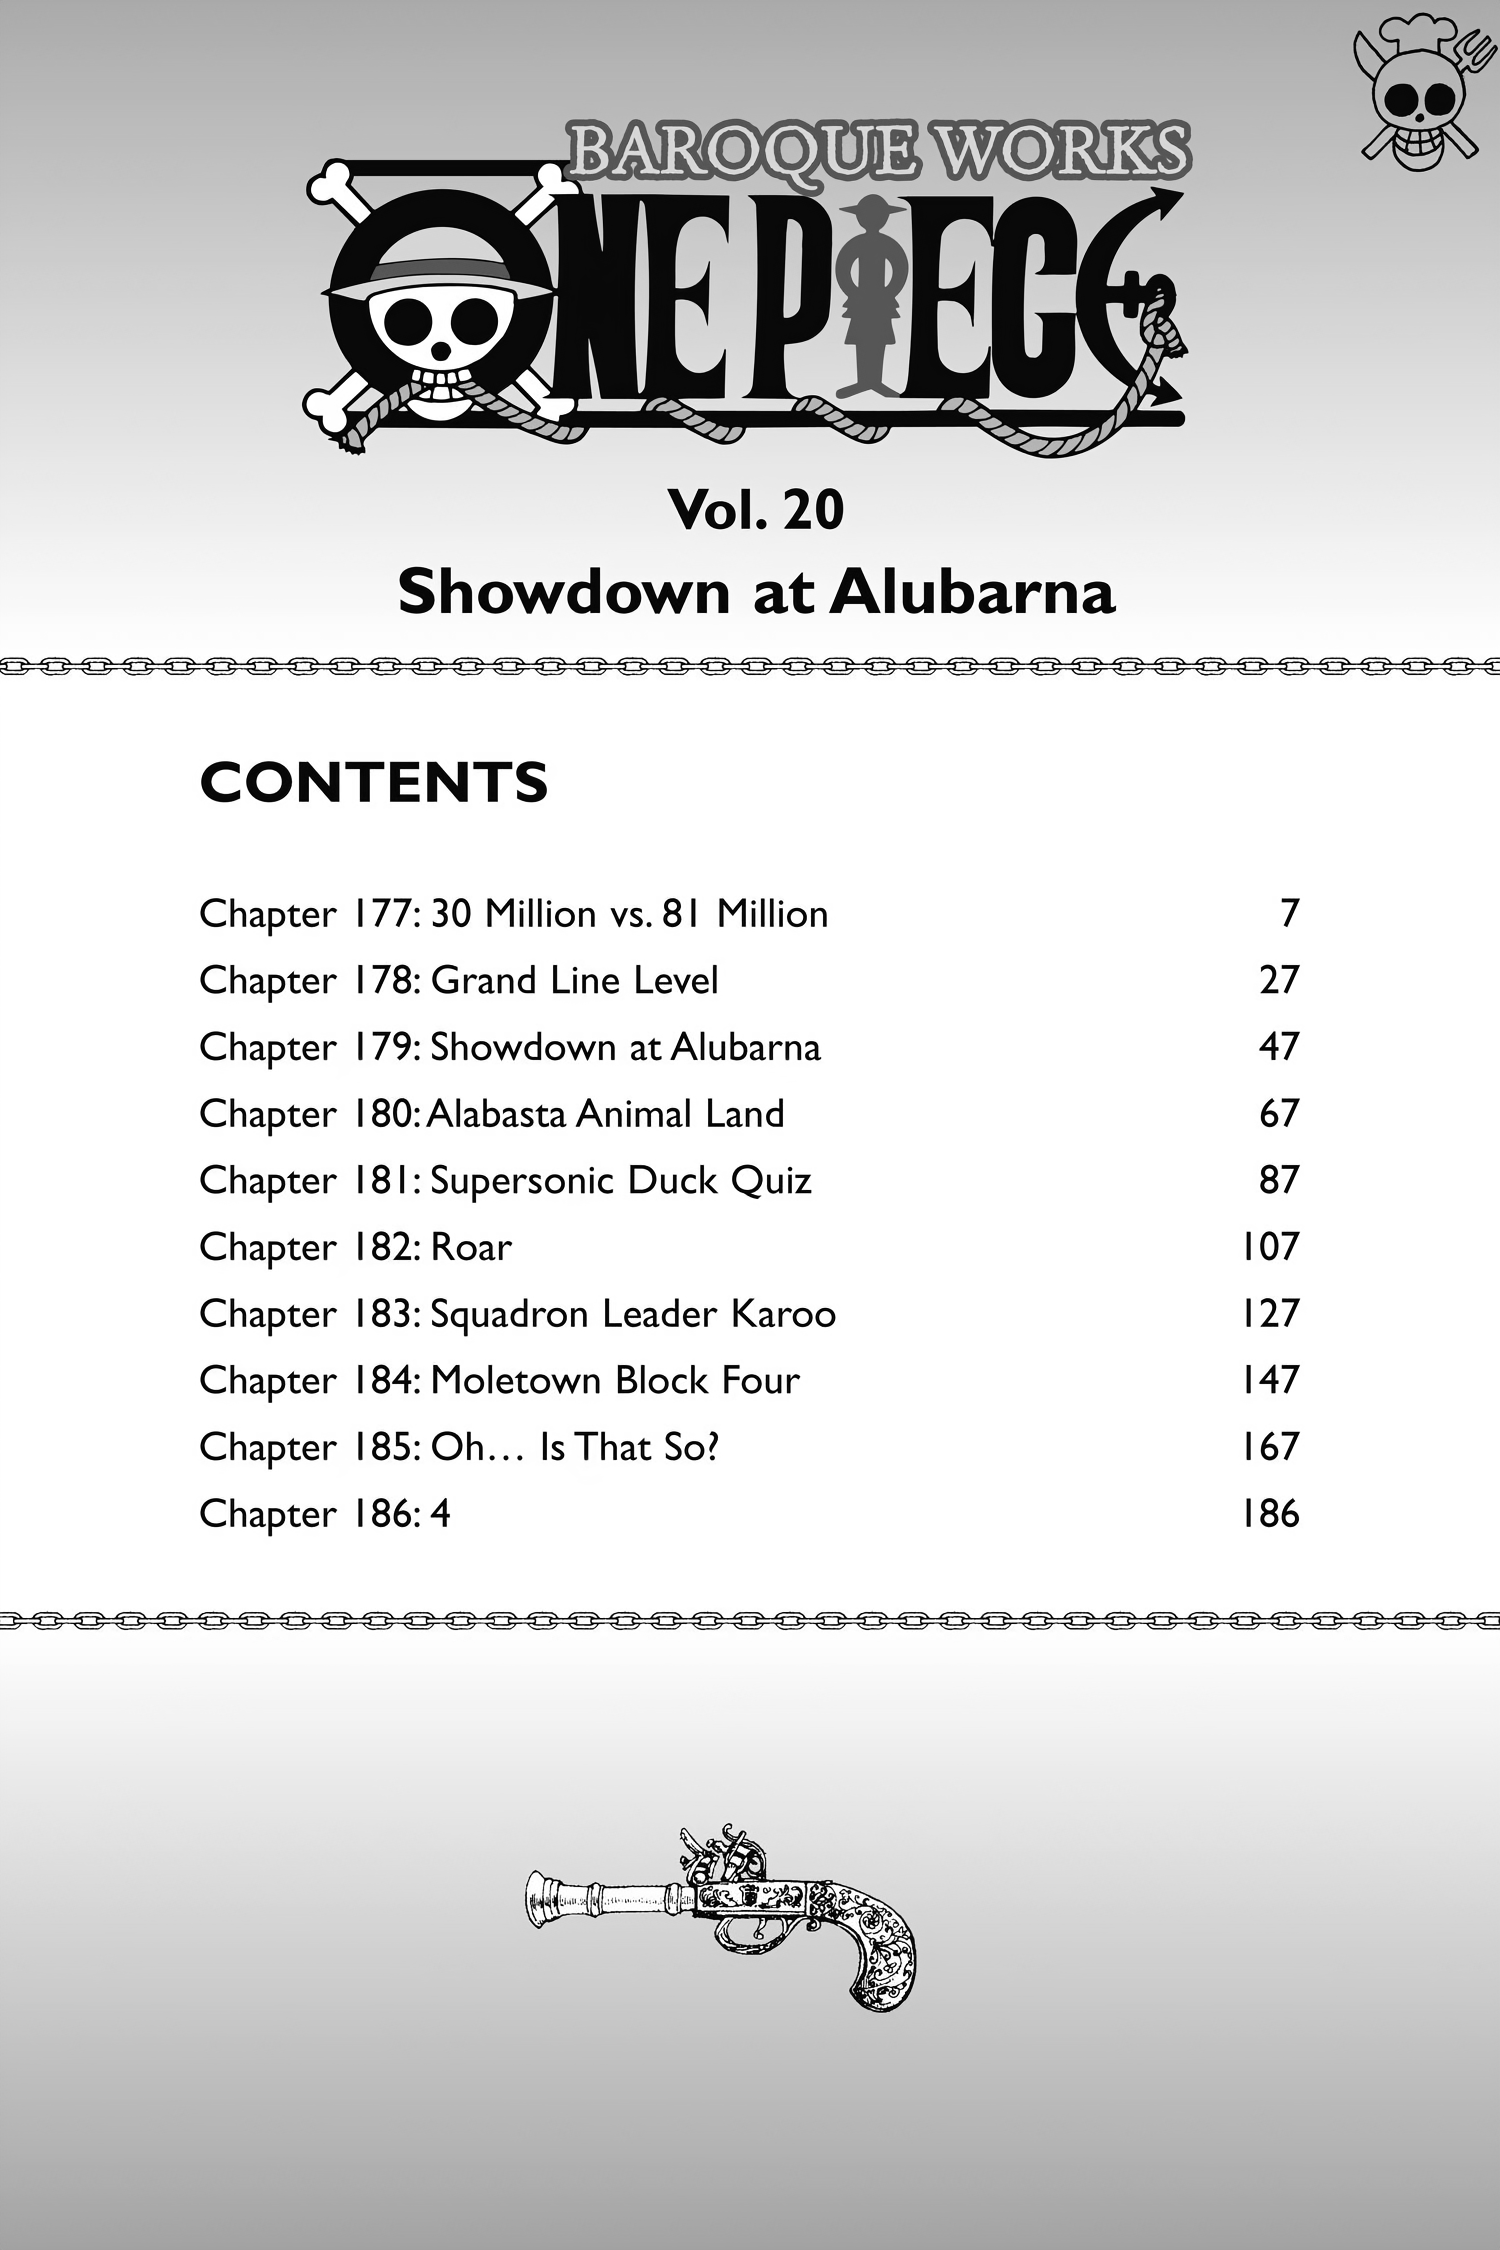
\includegraphics[width=\textwidth]{chapter/output/bad59.png}

    \end{subfigure}
    
    \caption{Bad pages as filtered out by the classifier}
    \label{fig:bad_images}
    
\end{figure}


This refined selection process ensured the model was trained on a focused dataset specifically containing relevant manga artwork. Through these collection and preprocessing steps, we prepared a high-quality, filtered and consistent dataset for our Cycle-GAN model.
\newpage

\section{Model Training}

\subsection{Training a cycle-GAN with UNET Generator}
Initially, we trained a deep UNET with 3 skip connections. The model consisted of multiple Squeeze Extract ResNet. The UNET Model had a total of
32212514 trainable parameters.We used PatchGAN as our discriminator. We trained the model on OnePiece Manga Dataset with Cycle-GAN architecture.
\\
We trained the model for 200 epoch with following parameters:
\begin{itemize}
        \item Learning rate for Color and BW Generators = 1e-4
        \item Learning rate for Color and BW Disciminator = 4e-4
        \item Batch Size = 2
        \item White Color Penalty Threshold = 0.8
        \item Input Image Width = 112
        \item Input Image Height = 112
        \item Model Initialization = Random Initialization
        \item Optimizer = Adam
        \item Adam Optimizer Betas = 0.5, 0.999
        \item Lambda Cycle = 10
\end{itemize}

We evaluated L1 loss, cycle consistency loss and adverserial loss during the training for both
generators and discriminators. Due to its architecture, U-Net Genrator was able to presever the features properly but failed to colorize the image as per our liking. Also, due to the complexity and depth of the generator, we could not accomodate images of size larger than 256x256 in the VRAM. \\
The losses and output during training of the generator is shown below.
\begin{figure}[bp]
    \centering
    \begin{subfigure}[b]{0.45\textwidth}
        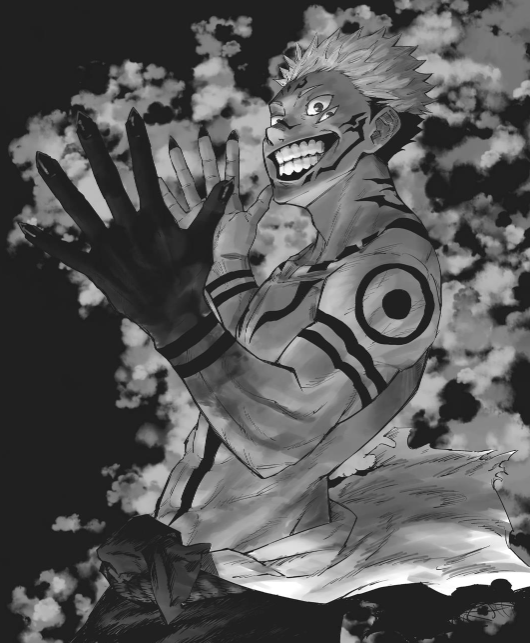
\includegraphics[height=0.8\textwidth]{chapter/output/UNetInput.png}
        \caption{Image Input to UNET}
    \end{subfigure}
    \hfill
    \begin{subfigure}[b]{0.45\textwidth}
        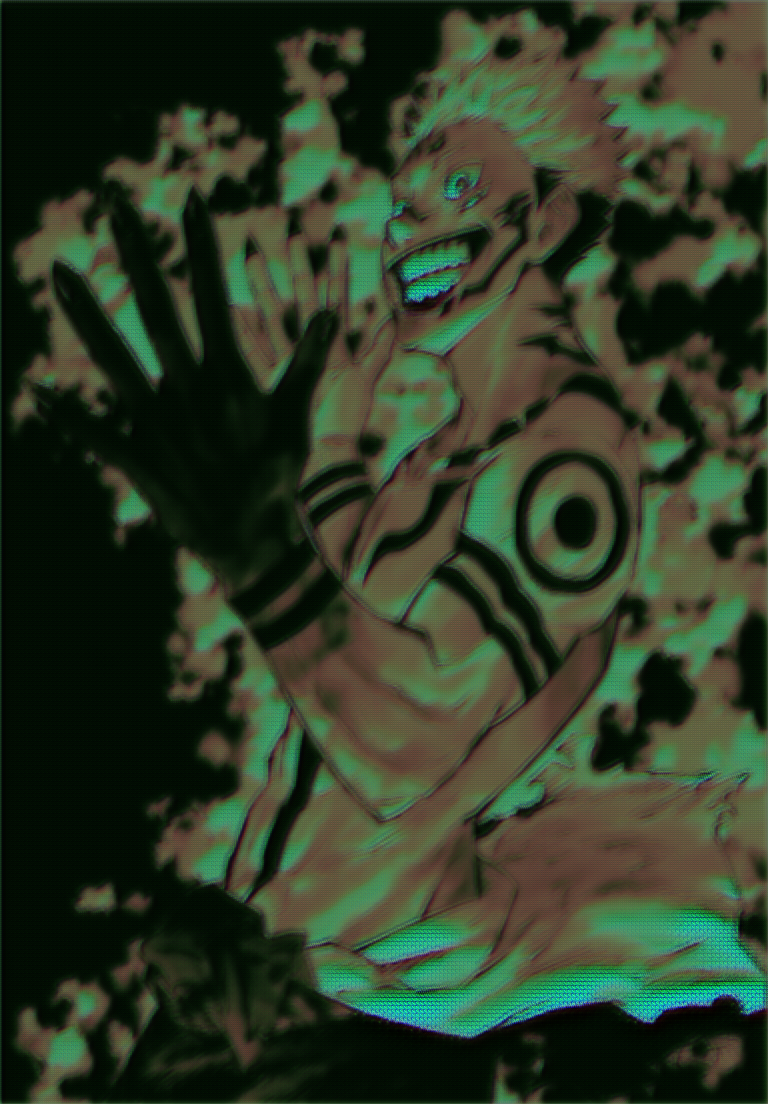
\includegraphics[height=0.8\textwidth]{chapter/output/UNet-output.png}
        \caption{Image Output from UNET}
    \end{subfigure}
    \caption{Output of UNET Generator}
    \label{fig:Output of UNET Generator}
\end{figure}
\newpage

\begin{figure}
    \centering
    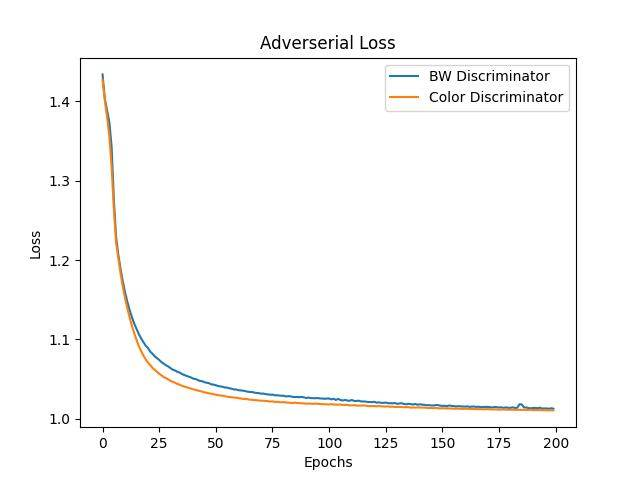
\includegraphics[width=0.7\textwidth]{chapter/output/UNet-adver.jpg}
    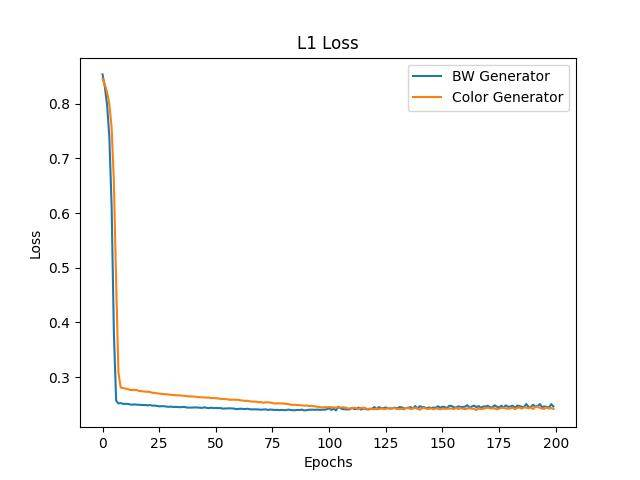
\includegraphics[width=0.7\textwidth]{chapter/output/UNet-l1.jpg}
    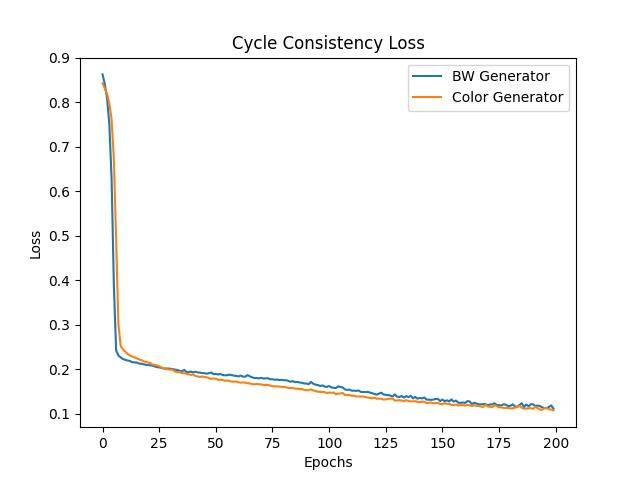
\includegraphics[width=0.7\textwidth]{chapter/output/UNet-cyclecon.jpg}
    \caption{Losses for generators and discriminators.}
    \label{Losses for generators and discriminators.}
\end{figure}
\clearpage


\subsection{Training a Cycle-GAN with Resnet9 Generator}
We realized the simpler ResNet9 generator architecture was able to preserve feature properly (not as much as U-net) and also should be able to colorize as per our liking.
We trained cycleGAN with a ResNet9 generator for both Color, and Black and White Generator. We used a 16x16 PatchGAN as the discriminator. Due to resource and training time constraints, we trained the model with 362 images in both domains from OnePiece Manga Dataset for 200 epochs.
\\
Initially, the images were resized without preserving the aspect ratio of original panel before passing to the model during training. The image outputs at an intermediate training stage have been given in \ref{fig:image_op_train}, which shows the loss of structural information due to resizing. Consequently, when using the so-trained model for inference, it was able to properly color resized images in the order of 256x256 and failed to appropriately fill larger images in original size or aspect ratio. 

So, the model was trained on unresized and cropped images with following parameters.
\begin{itemize}
    \item Number of Epoch = 200
    \item Batch Size = 1
    \item Learning Rate for Generator = 0.0002
    \item Learning Rate for Discriminator = 0.0002
    \item Input Image Width = 256
    \item Input Image Height = 256
    \item Model Initialization = Normal Initialization
    \item Initialization Gain = 0.02
    \item Optimizer = Adam
    \item Adam Optimizer Betas = 0.5, 0.999
    \item Lambda Cycle = 10
    \item Normalization = Instance Normalization
\end{itemize}
\newpage
\begin{figure}
    \centering
      \begin{subfigure}[b]{0.3\textwidth}
        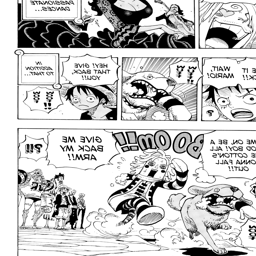
\includegraphics[width=\textwidth]{chapter/output/epoch100_real_A.png}
        \caption{Real BW}
    \end{subfigure}  
    \hfill
    \begin{subfigure}[b]{0.3\textwidth}
        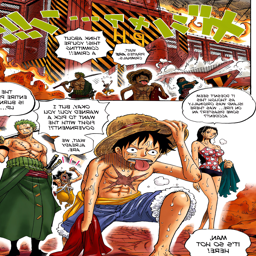
\includegraphics[width=\textwidth]{chapter/output/epoch100_real_B.png}
        \caption{Real Color}
    \end{subfigure}
\end{figure}

\begin{figure}
\centering
    \begin{subfigure}[b]{0.3\textwidth}
        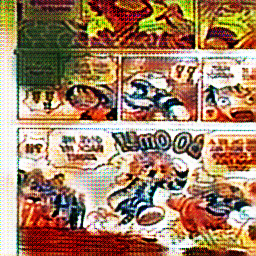
\includegraphics[width=\textwidth]{chapter/output/epoch100_fake_B.png}
        \caption{Fake Color}
    \end{subfigure}
    \hfill
    \begin{subfigure}[b]{0.3\textwidth}
        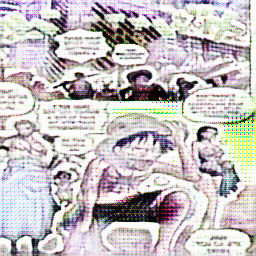
\includegraphics[width=\textwidth]{chapter/output/epoch100_fake_A.png}
        \caption{Fake BW}
    \end{subfigure}

\end{figure}

\begin{figure}
    \centering

    \begin{subfigure}[b]{0.3\textwidth}
        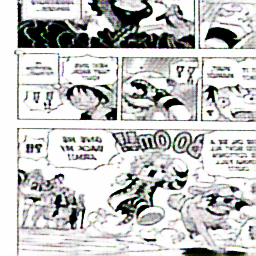
\includegraphics[width=\textwidth]{chapter/output/epoch100_idt_B.png}
       \caption{Identity BW}
    \end{subfigure}
    \hfill
    \begin{subfigure}[b]{0.3\textwidth}
        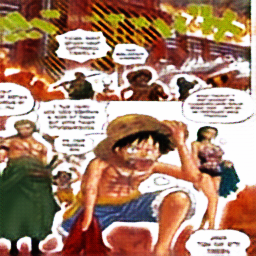
\includegraphics[width=\textwidth]{chapter/output/epoch100_idt_A.png}
        \caption{Identity Color}
    \end{subfigure}

\end{figure}



\begin{figure}  
    \centering
    \begin{subfigure}[b]{0.3\textwidth}
        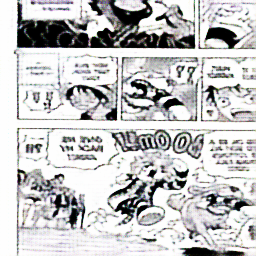
\includegraphics[width=\textwidth]{chapter/output/epoch100_rec_A.png}
        \caption{Recreated BW}
    \end{subfigure}
    \hfill
    \begin{subfigure}[b]{0.3\textwidth}
        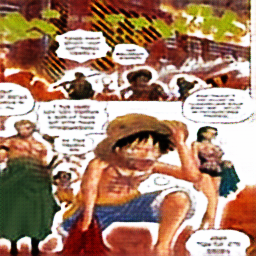
\includegraphics[width=\textwidth]{chapter/output/epoch100_rec_B.png}
        \caption{Recreated Color}
    \end{subfigure}
    
    \caption{Images output during training}
    \label{fig:bad_images}
    
\end{figure}

%---------------------------------gen flowchart
\begin{figure}[hbtp]
  \centering
  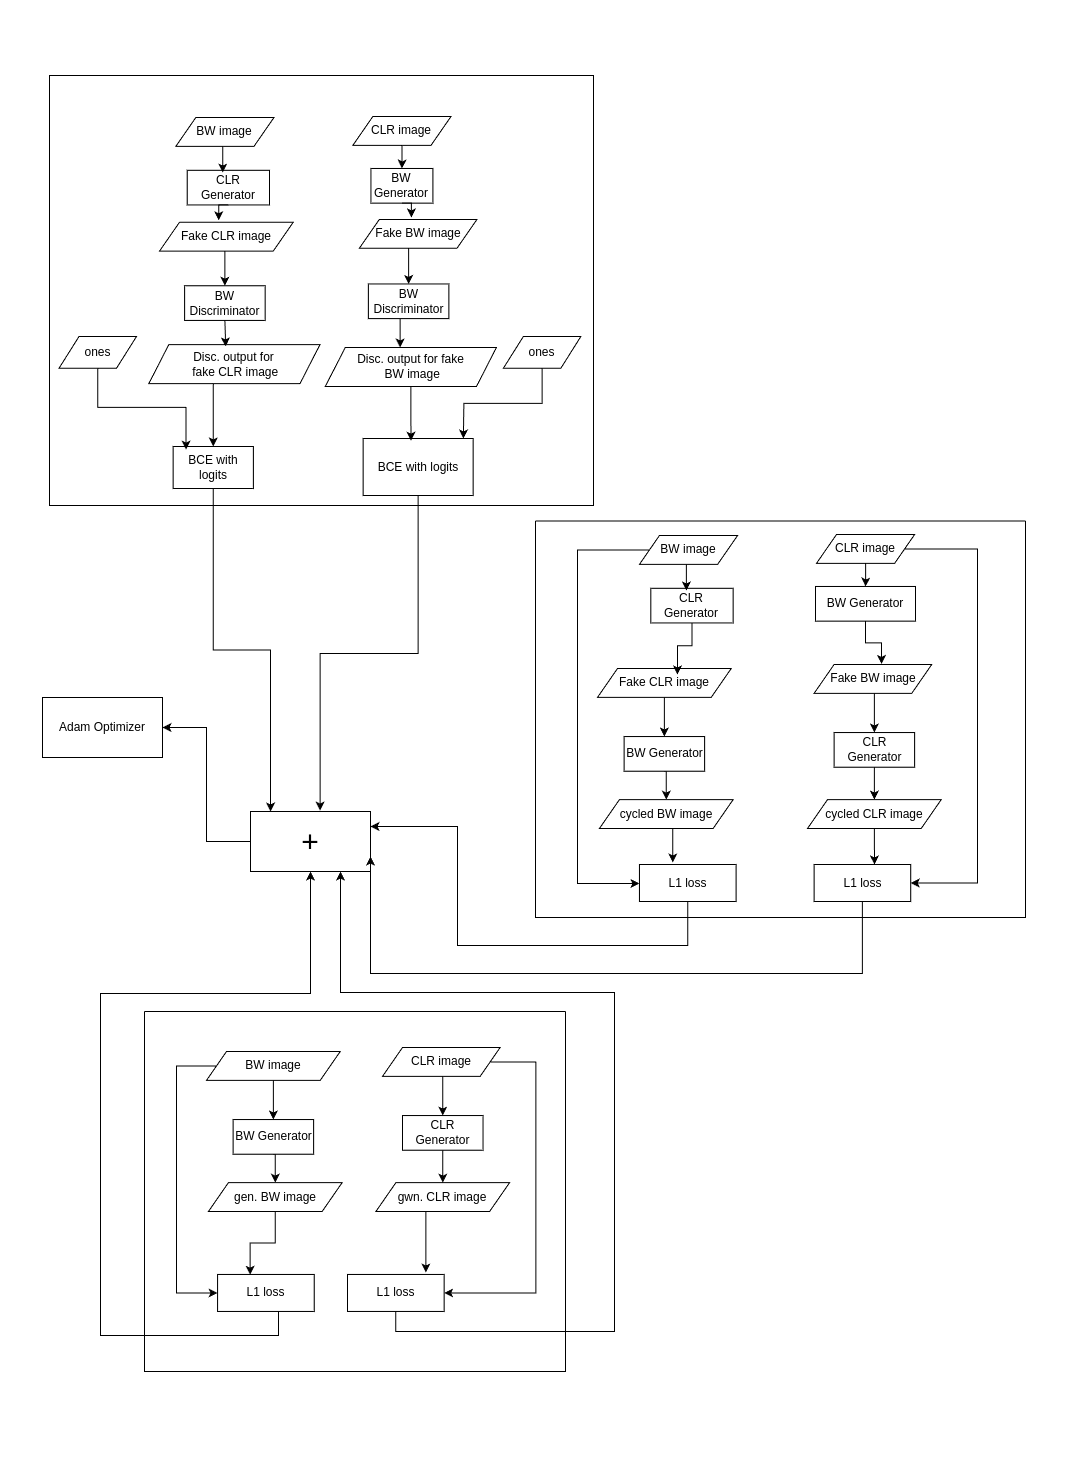
\includegraphics[width=1.1\textwidth]{chapter/img_procedure/generator_procedure_full.png}
  \caption{Generator Training Procedure }
  \label{Generator Training Procedure}
\end{figure}
%--------------------------------- disc flowchart

\begin{figure}[hbtp]
  \centering
  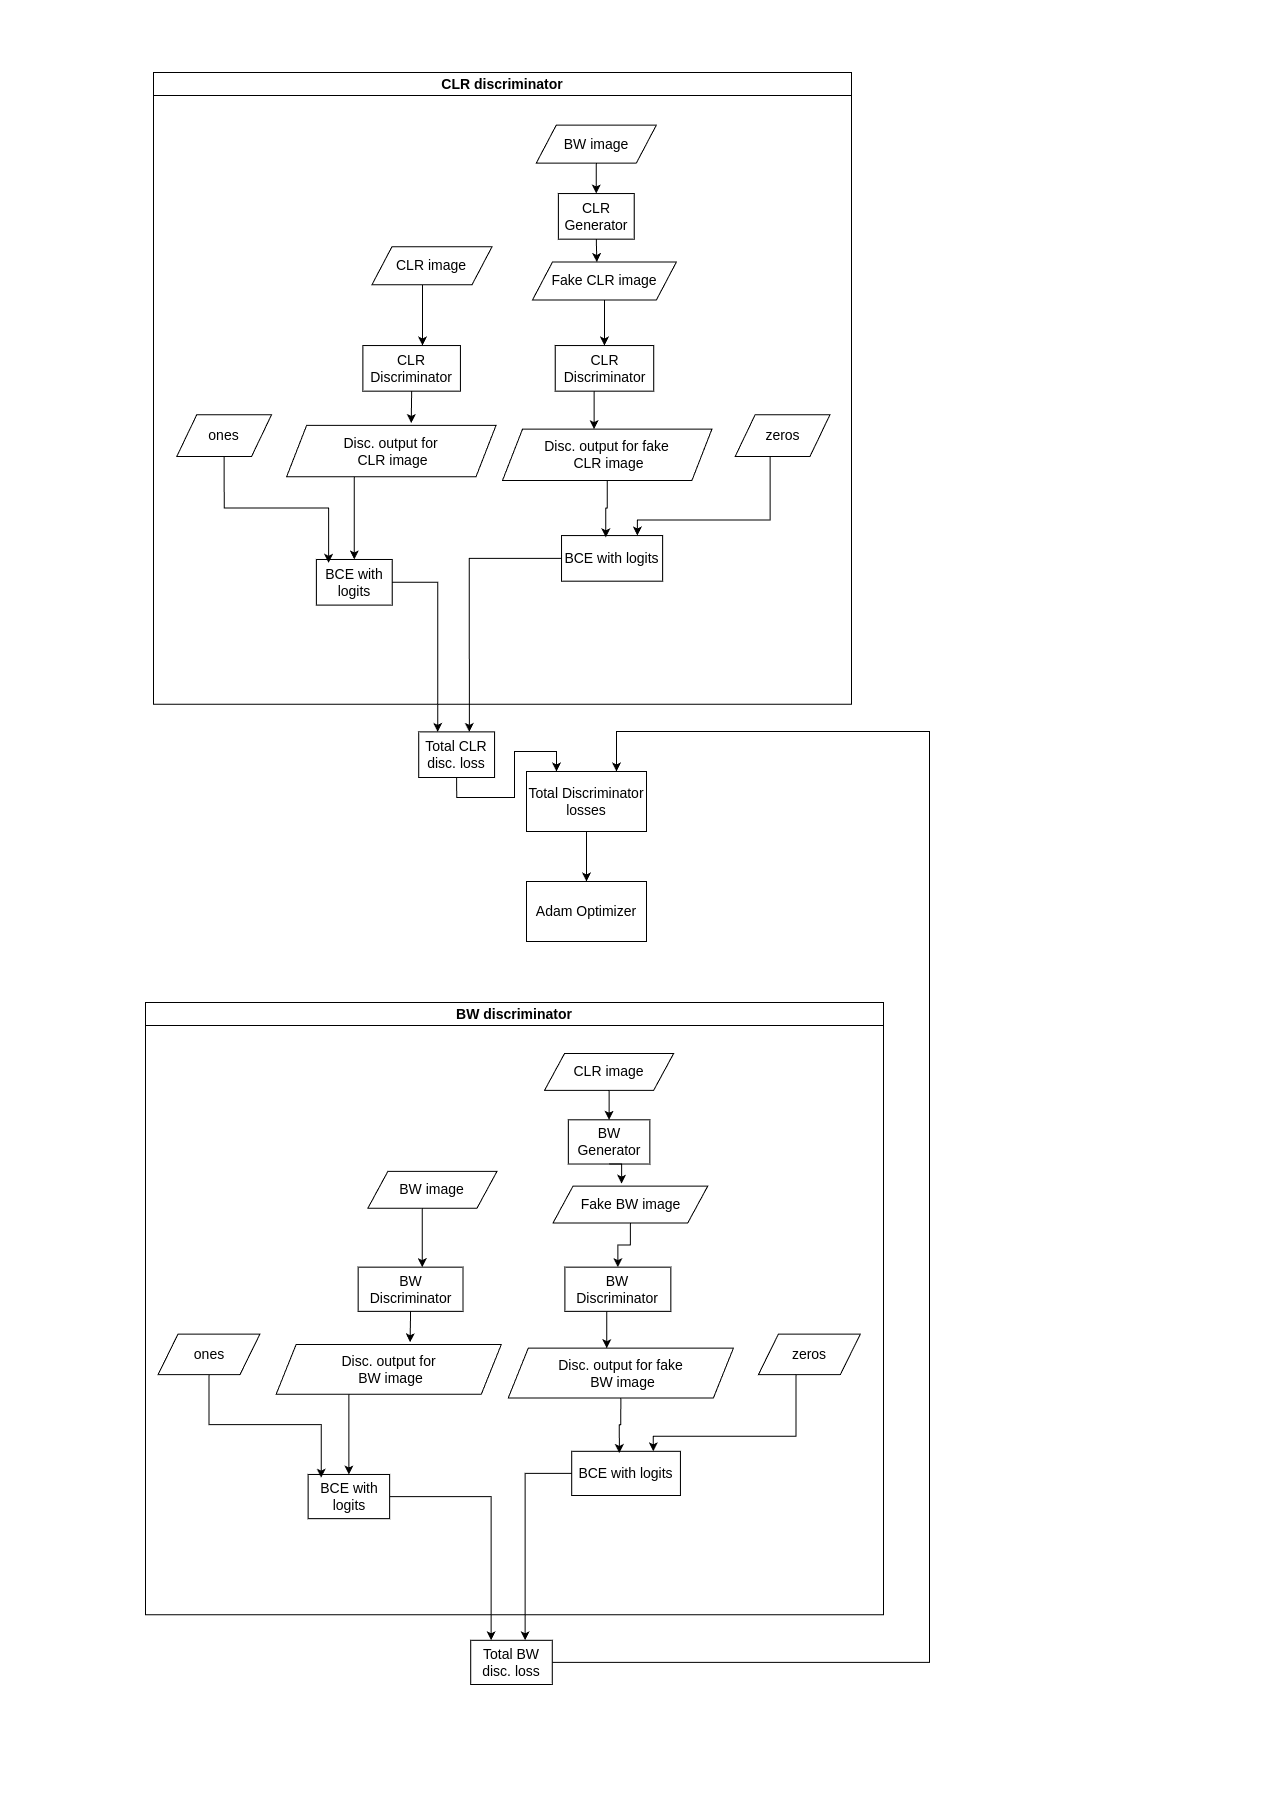
\includegraphics[width=1.2\textwidth]{chapter/img_procedure/disc_procedure_full.png}
  \caption{Discriminator Training Procedure }
  \label{Discriminator Training Procedure}
\end{figure}
%-----------------------------------------------------

\begin{figure}[htbp]
    \centering
    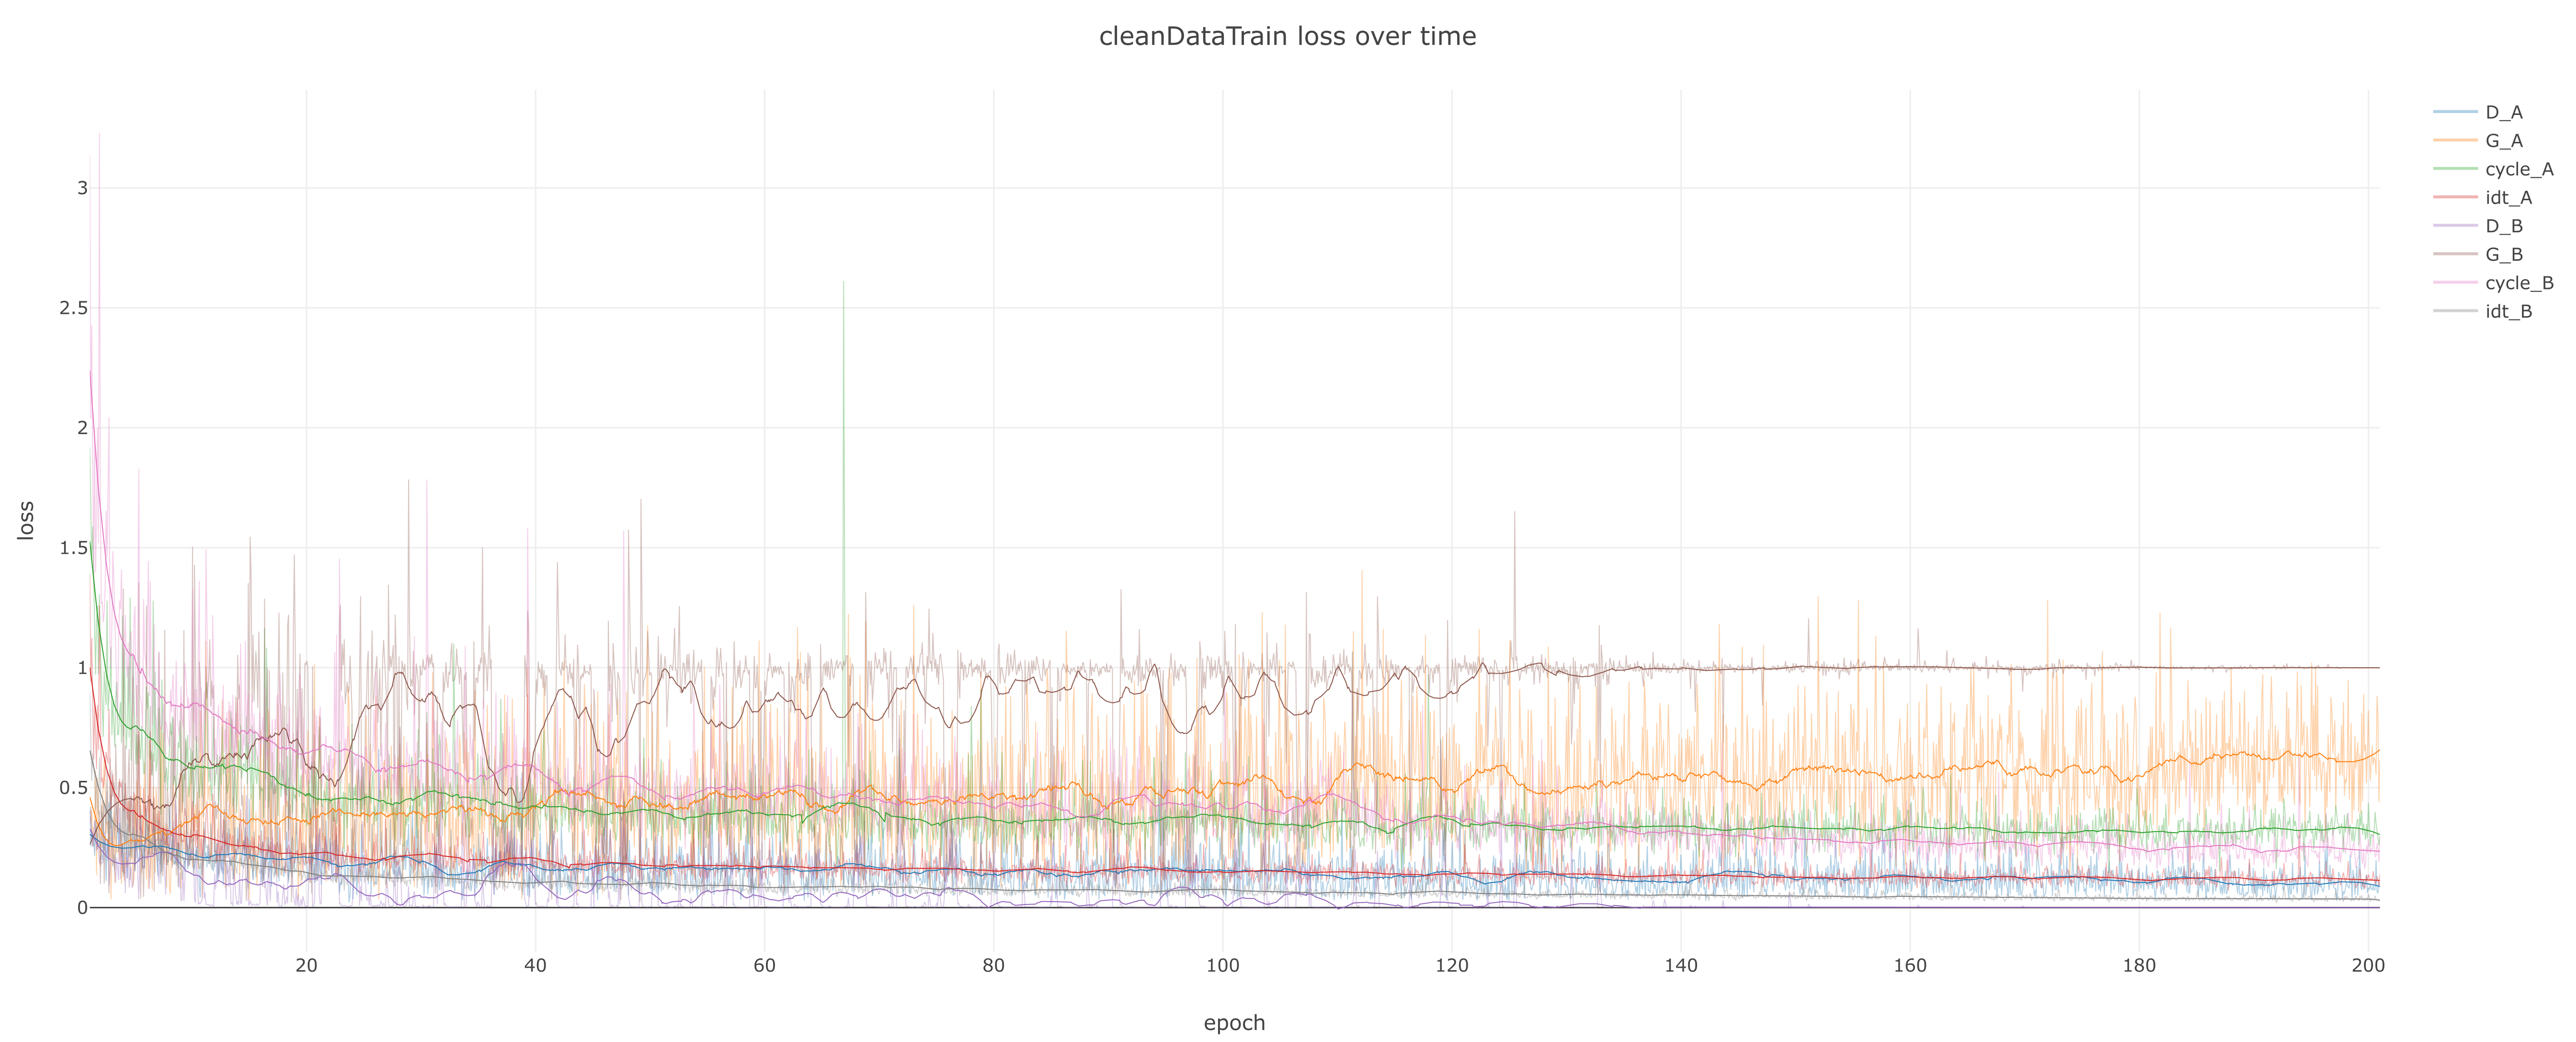
\includegraphics[width=1\textwidth]{chapter/losses_png/all.png}
    \caption{Losses for training with ResNet9Generator and PatchGAN}

    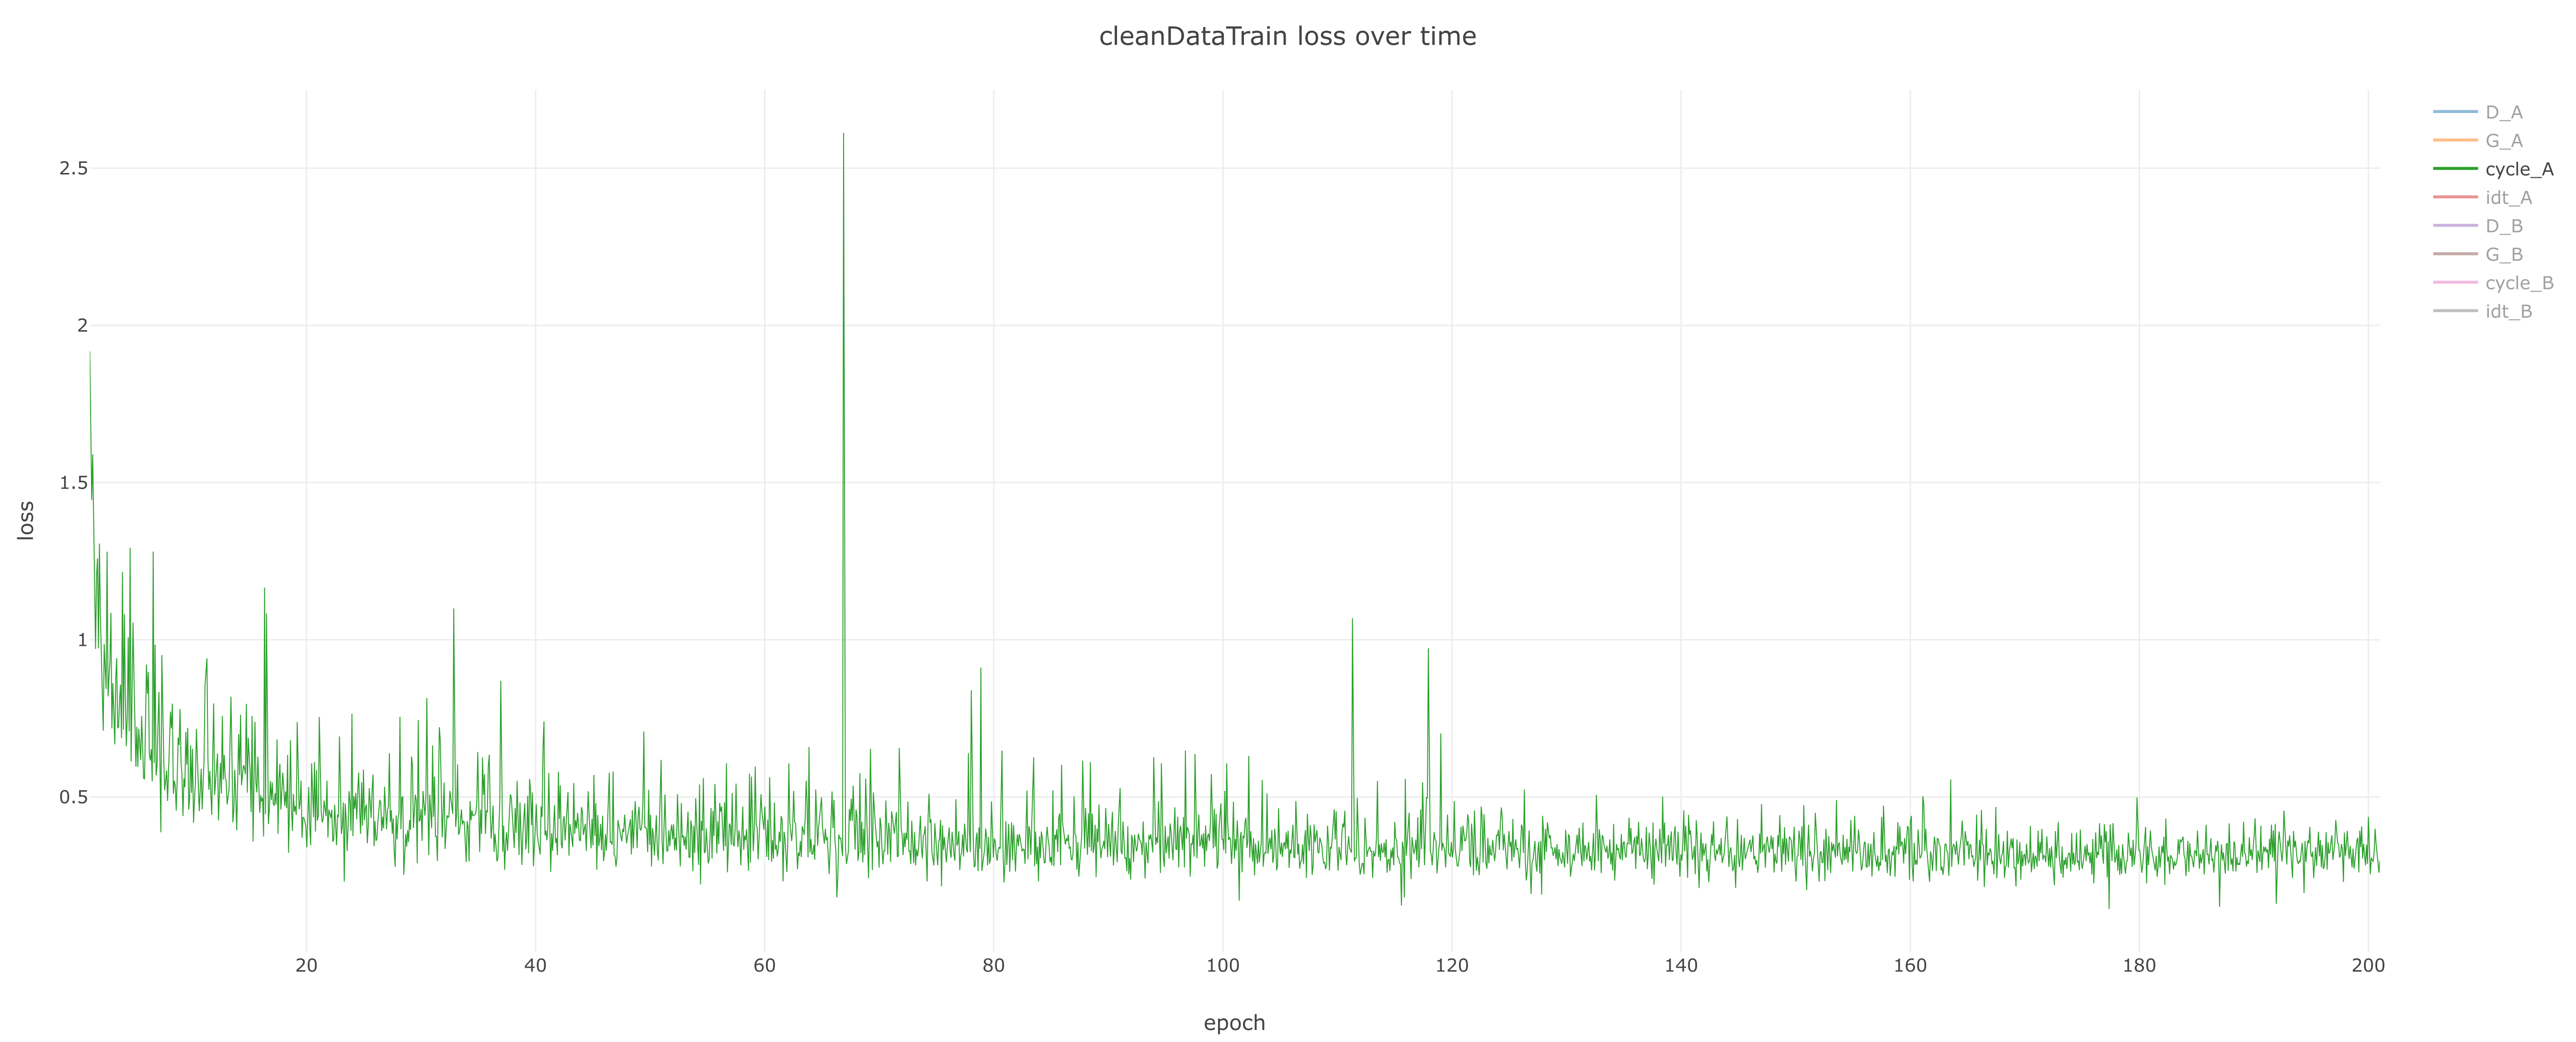
\includegraphics[width=1\textwidth]{chapter/losses_png/cycle_a.png}
    \caption{Cycle Consistency Loss (L1) for Color Generator}
    
    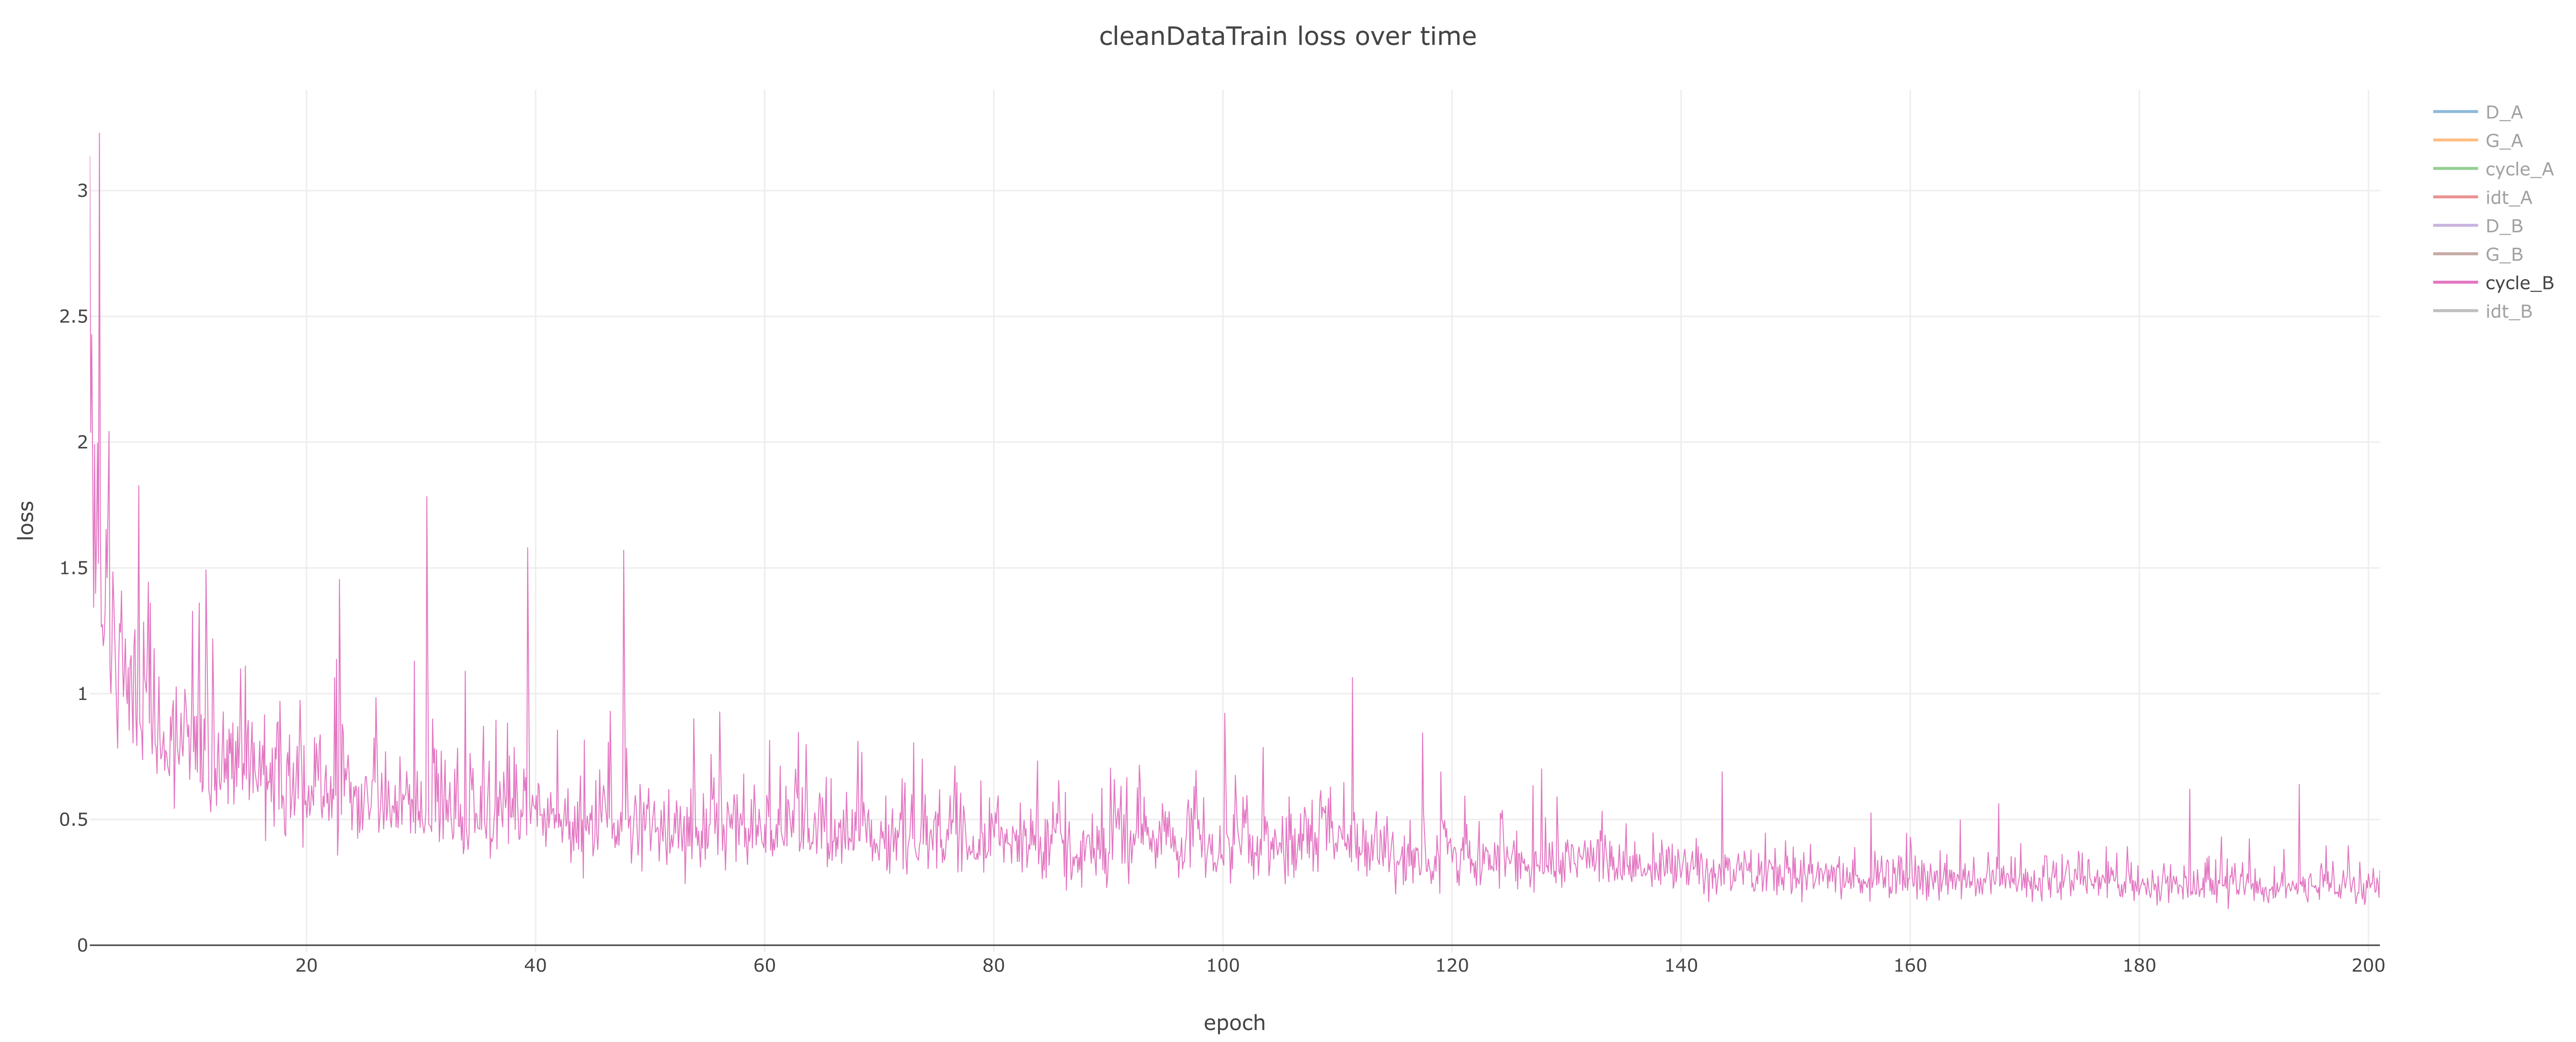
\includegraphics[width=1\textwidth]{chapter/losses_png/cycle_b.png}
    \caption{Cycle Consistency Loss (L1) for BW Generator}
    \end{figure}
    \pagebreak
    \newpage
    \begin{figure}[htbp]
    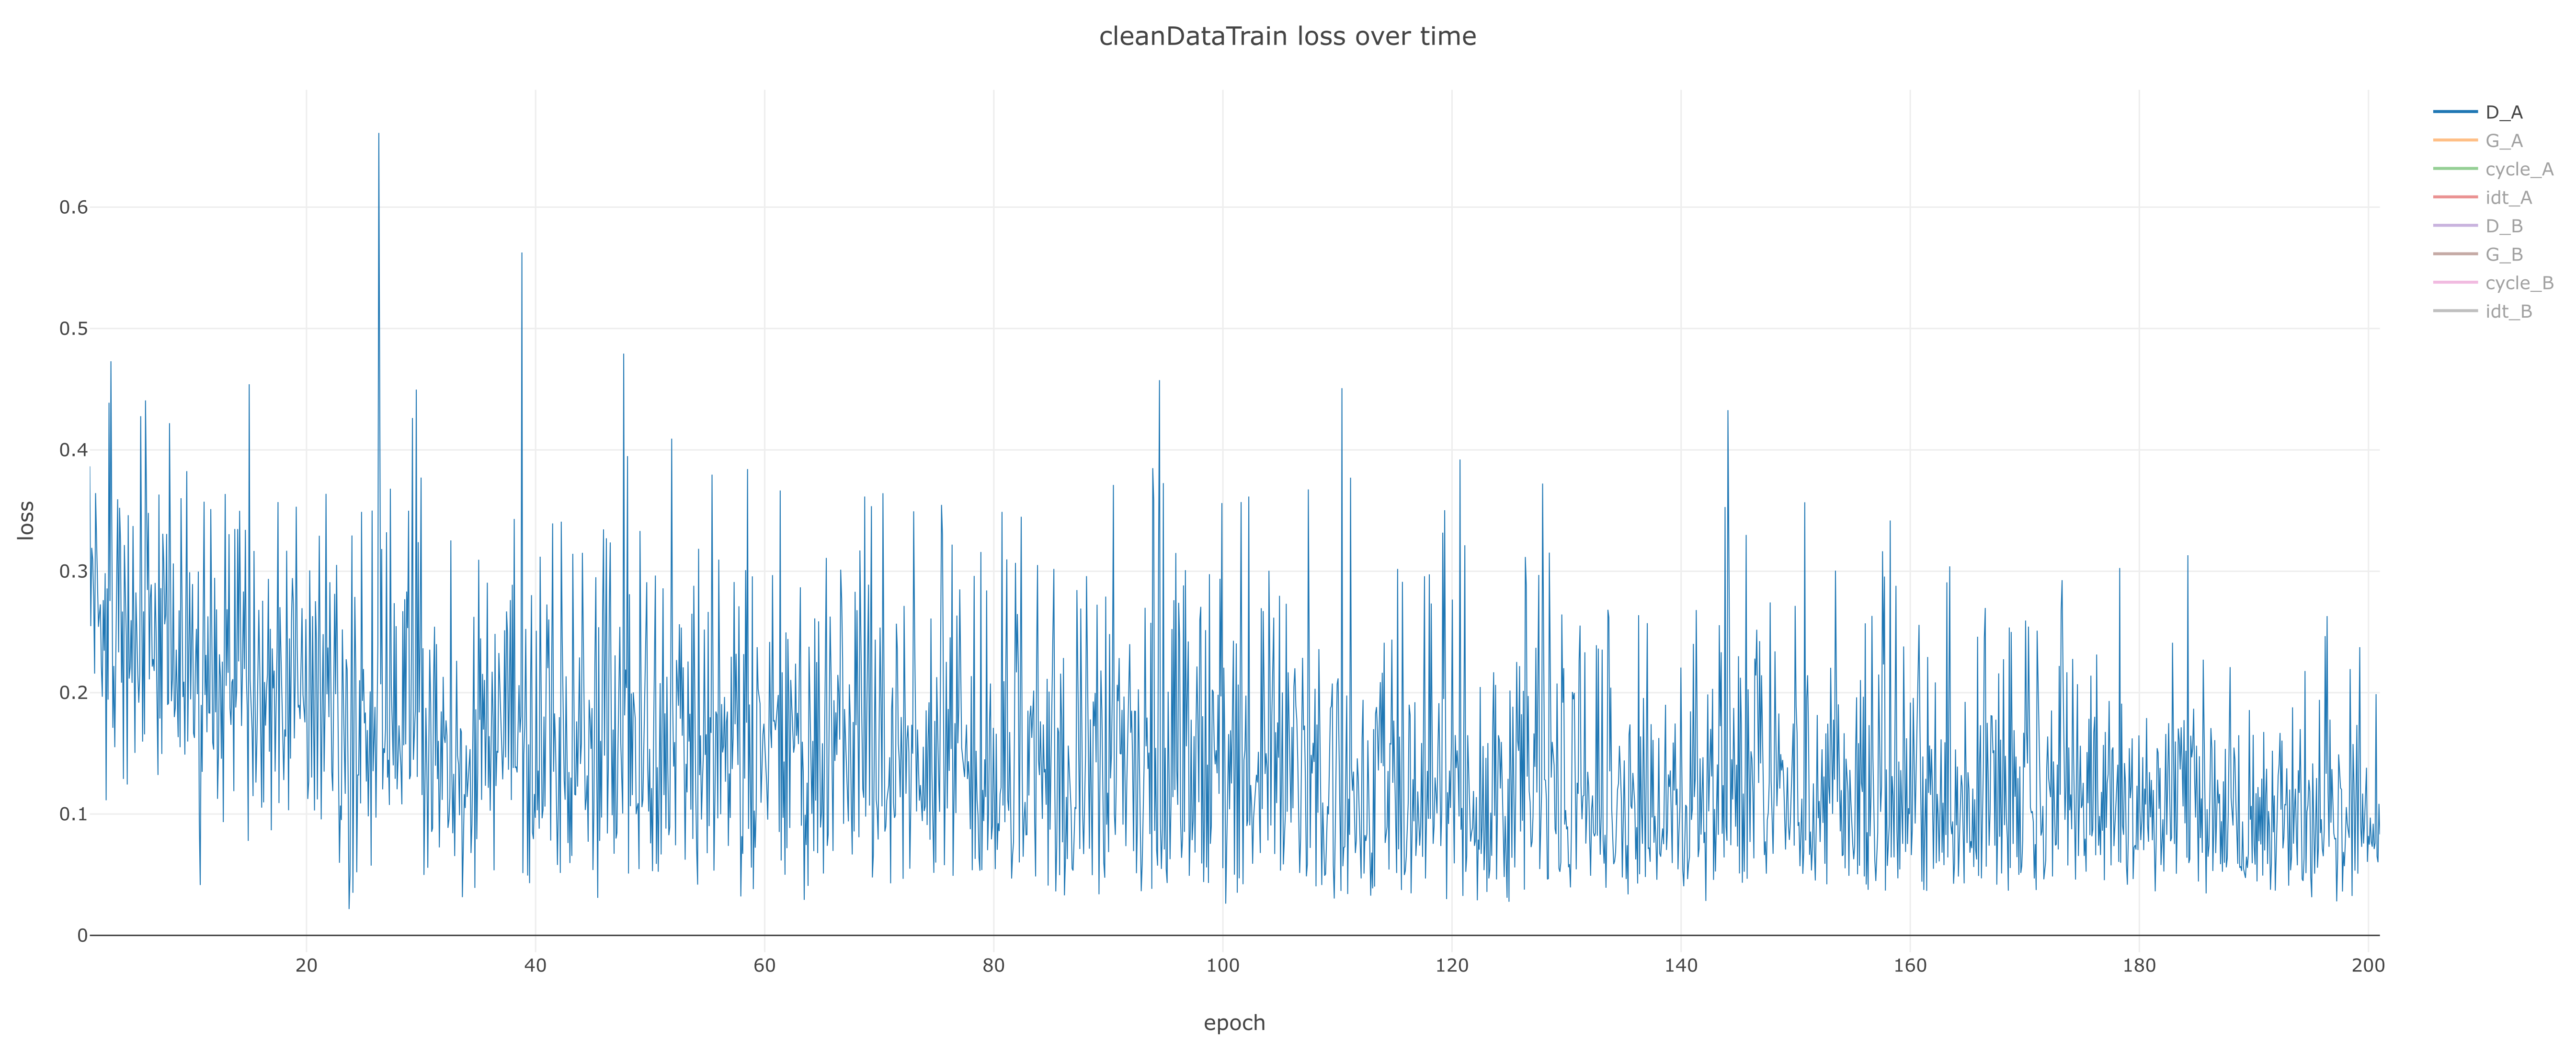
\includegraphics[width=1\textwidth]{chapter/losses_png/d_a.png}
    \caption{BCE Loss for Color Discriminator}
    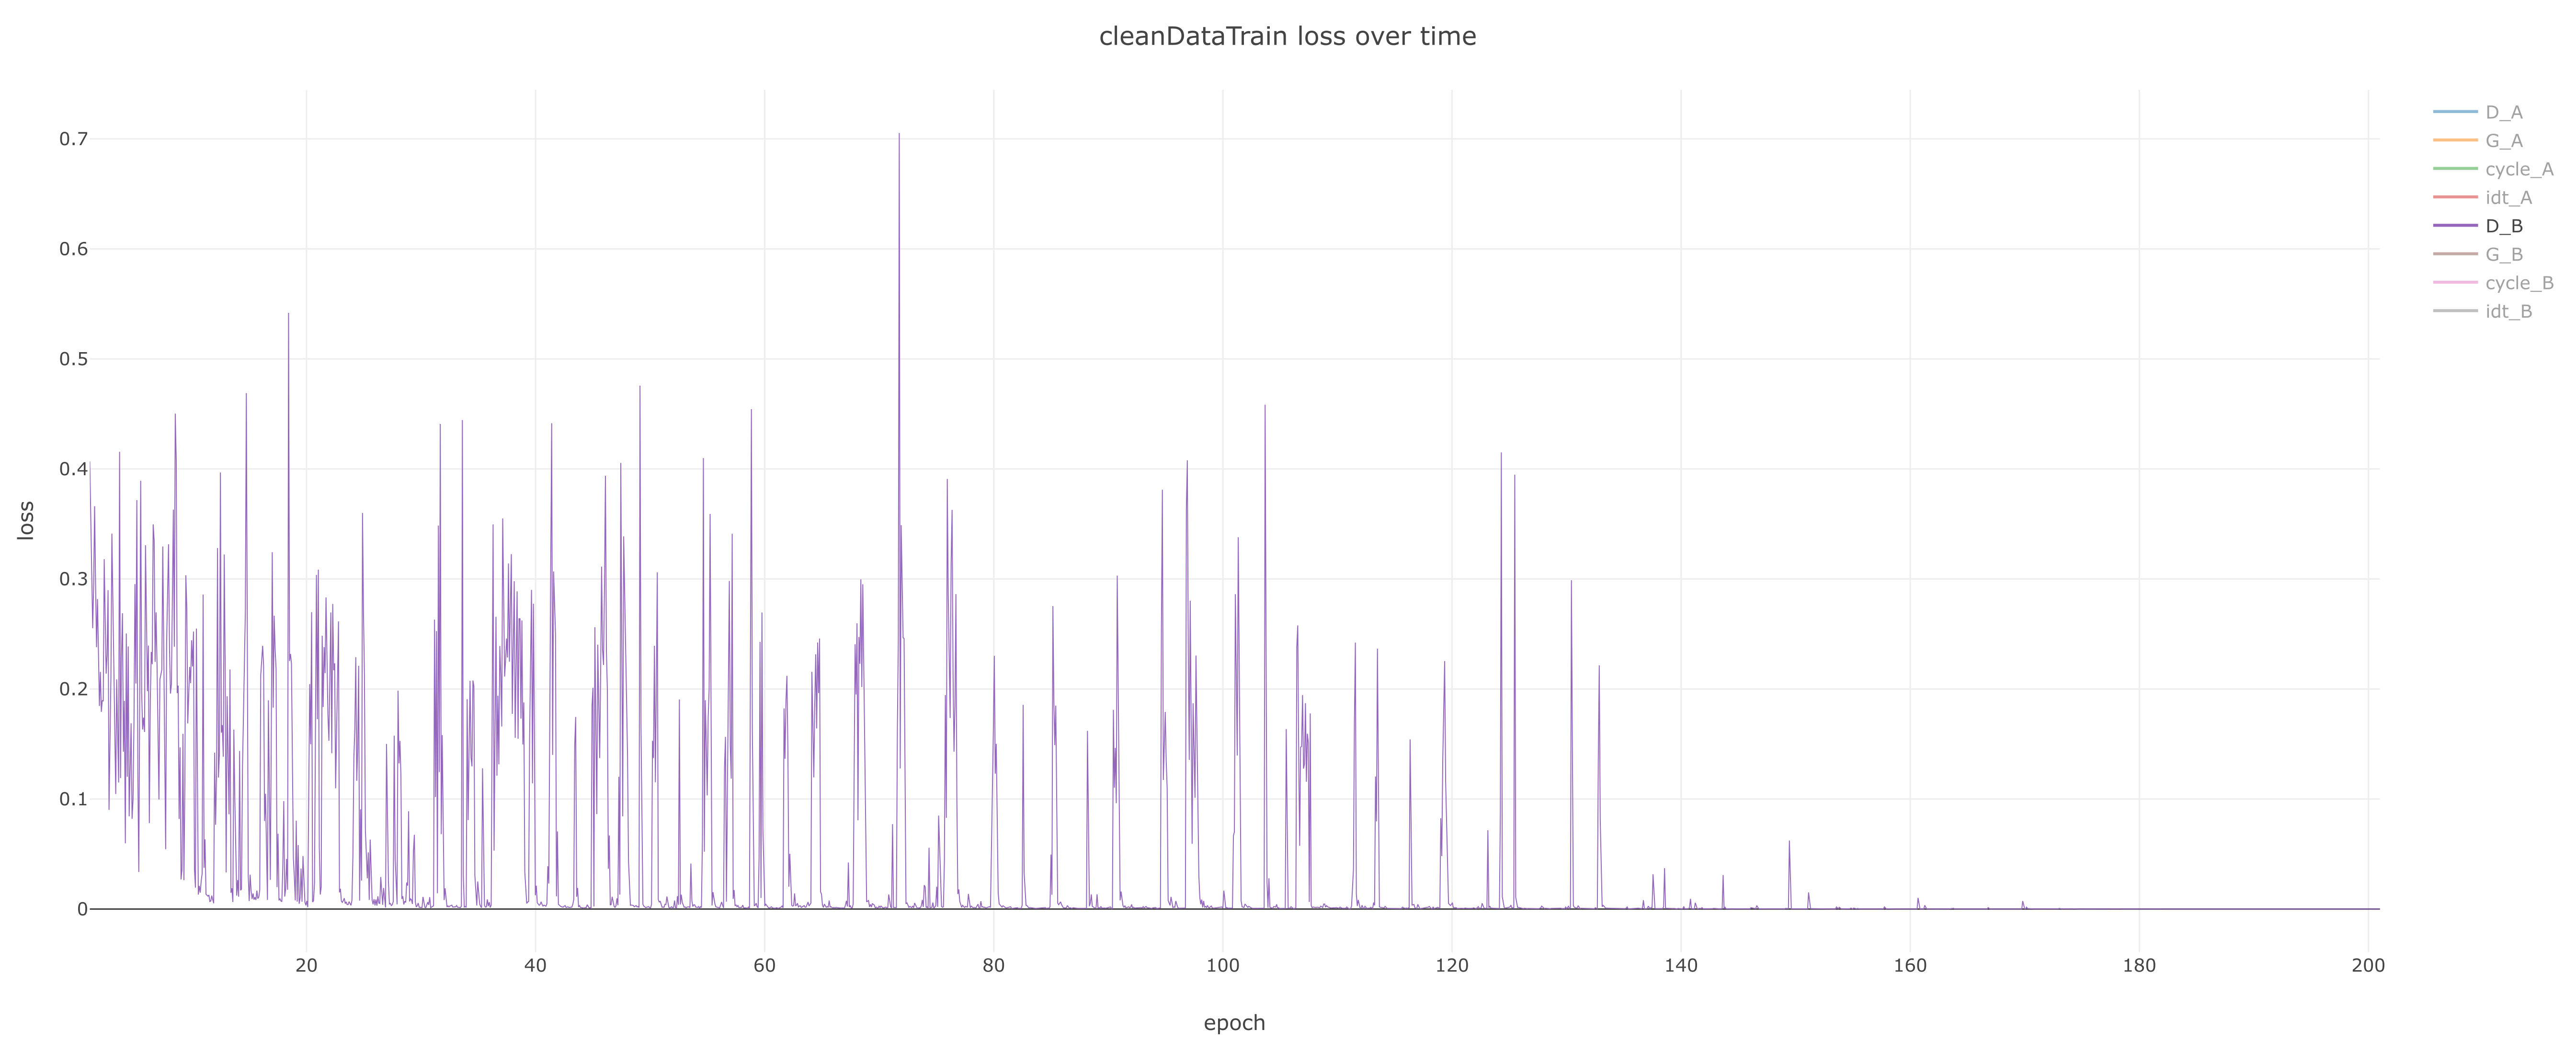
\includegraphics[width=1\textwidth]{chapter/losses_png/d_b.png}
    \caption{BCE Loss for BW Discriminator}
    
    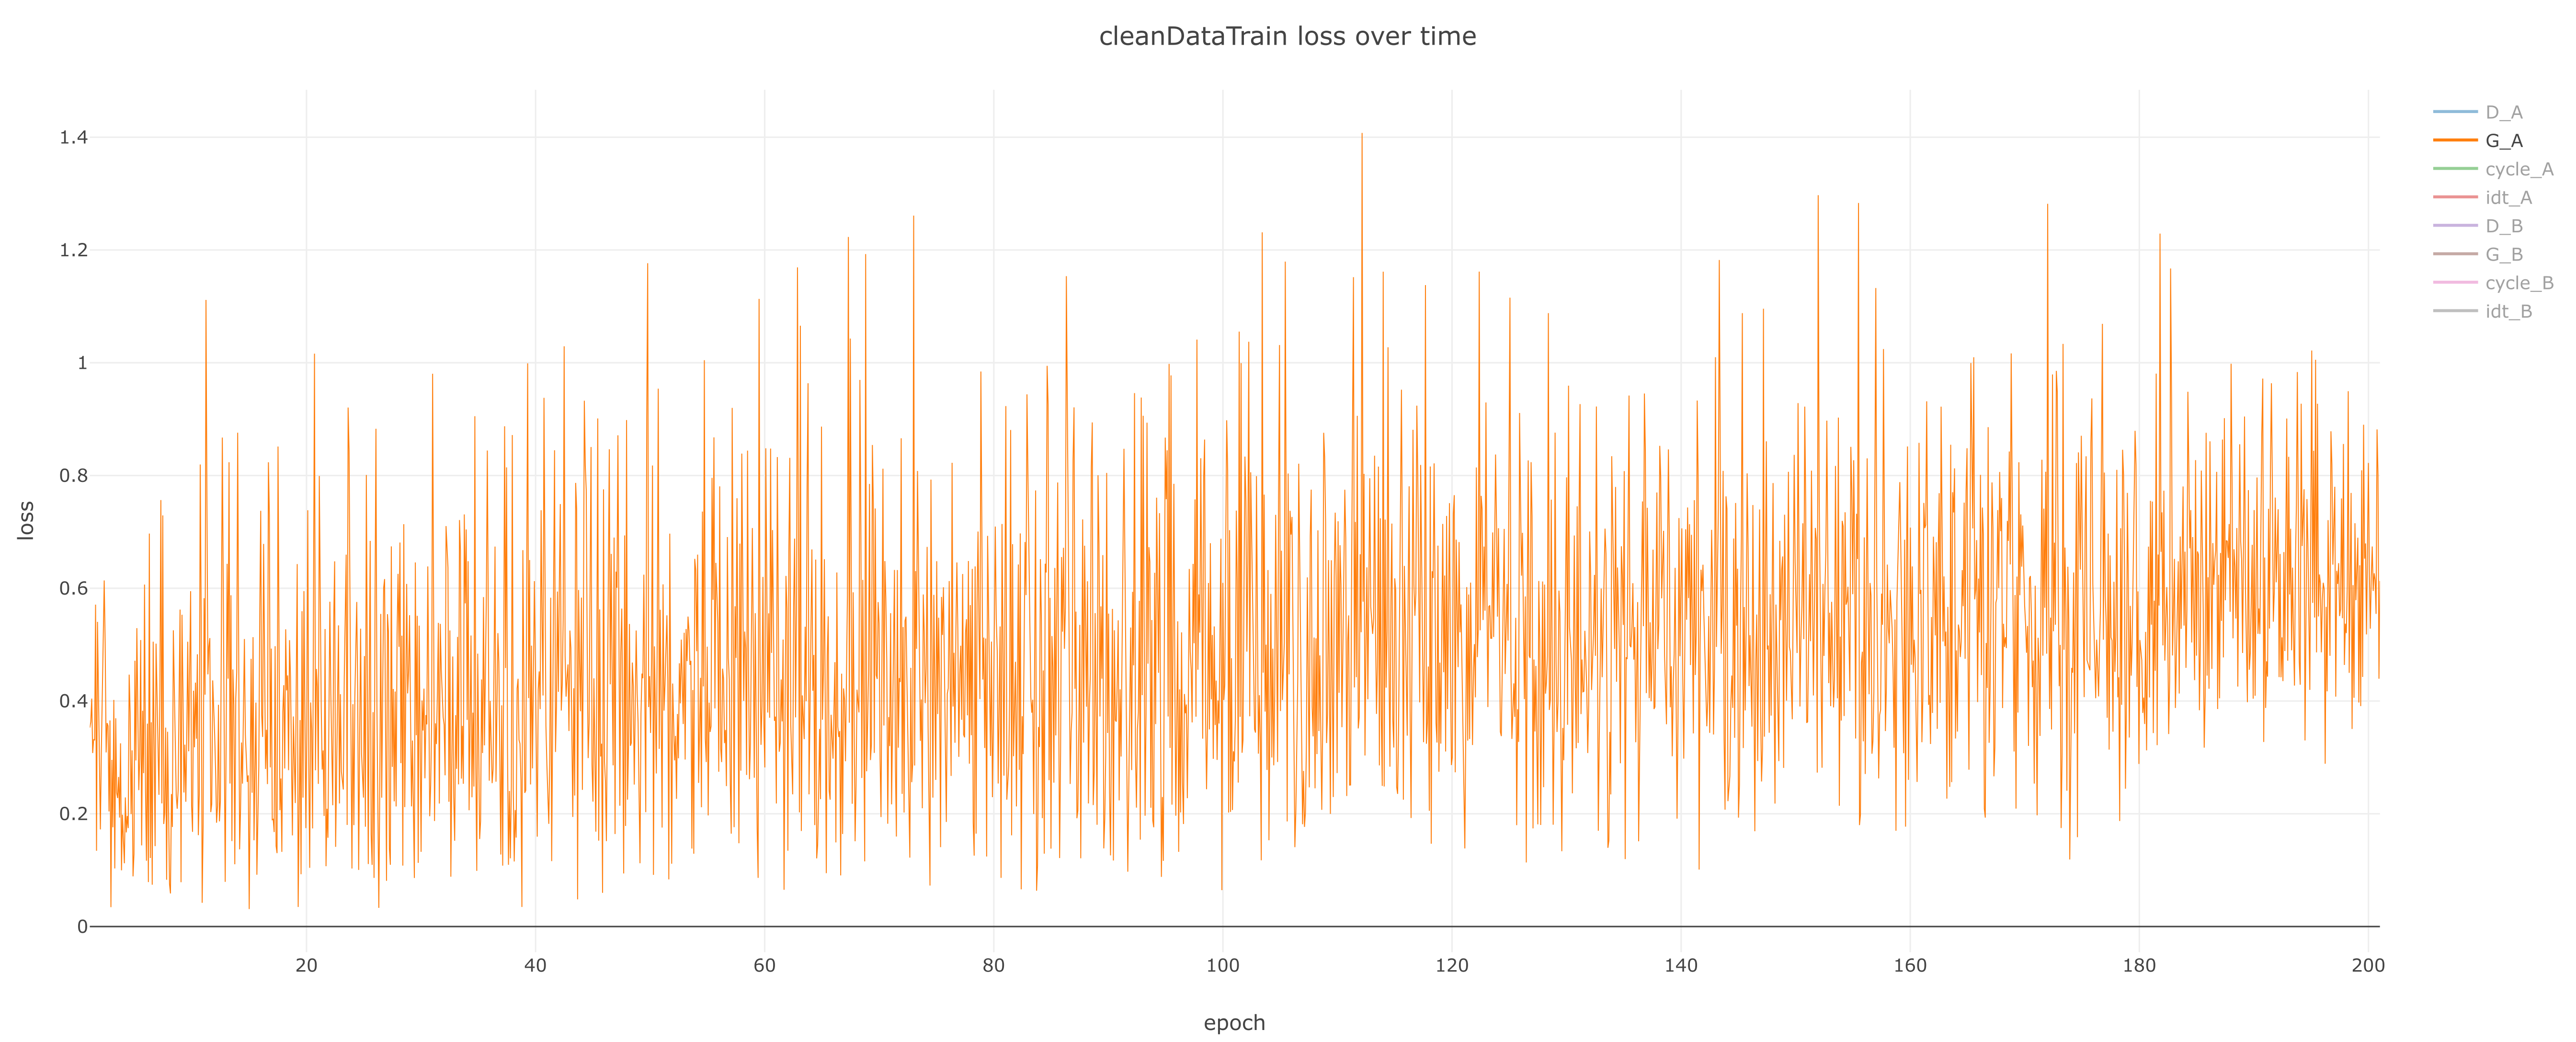
\includegraphics[width=1\textwidth]{chapter/losses_png/g_a.png}
    \caption{Adversarial (BCE) Loss for Color Generator}
     \end{figure}
    \pagebreak
    \newpage
    \begin{figure}[htbp]
    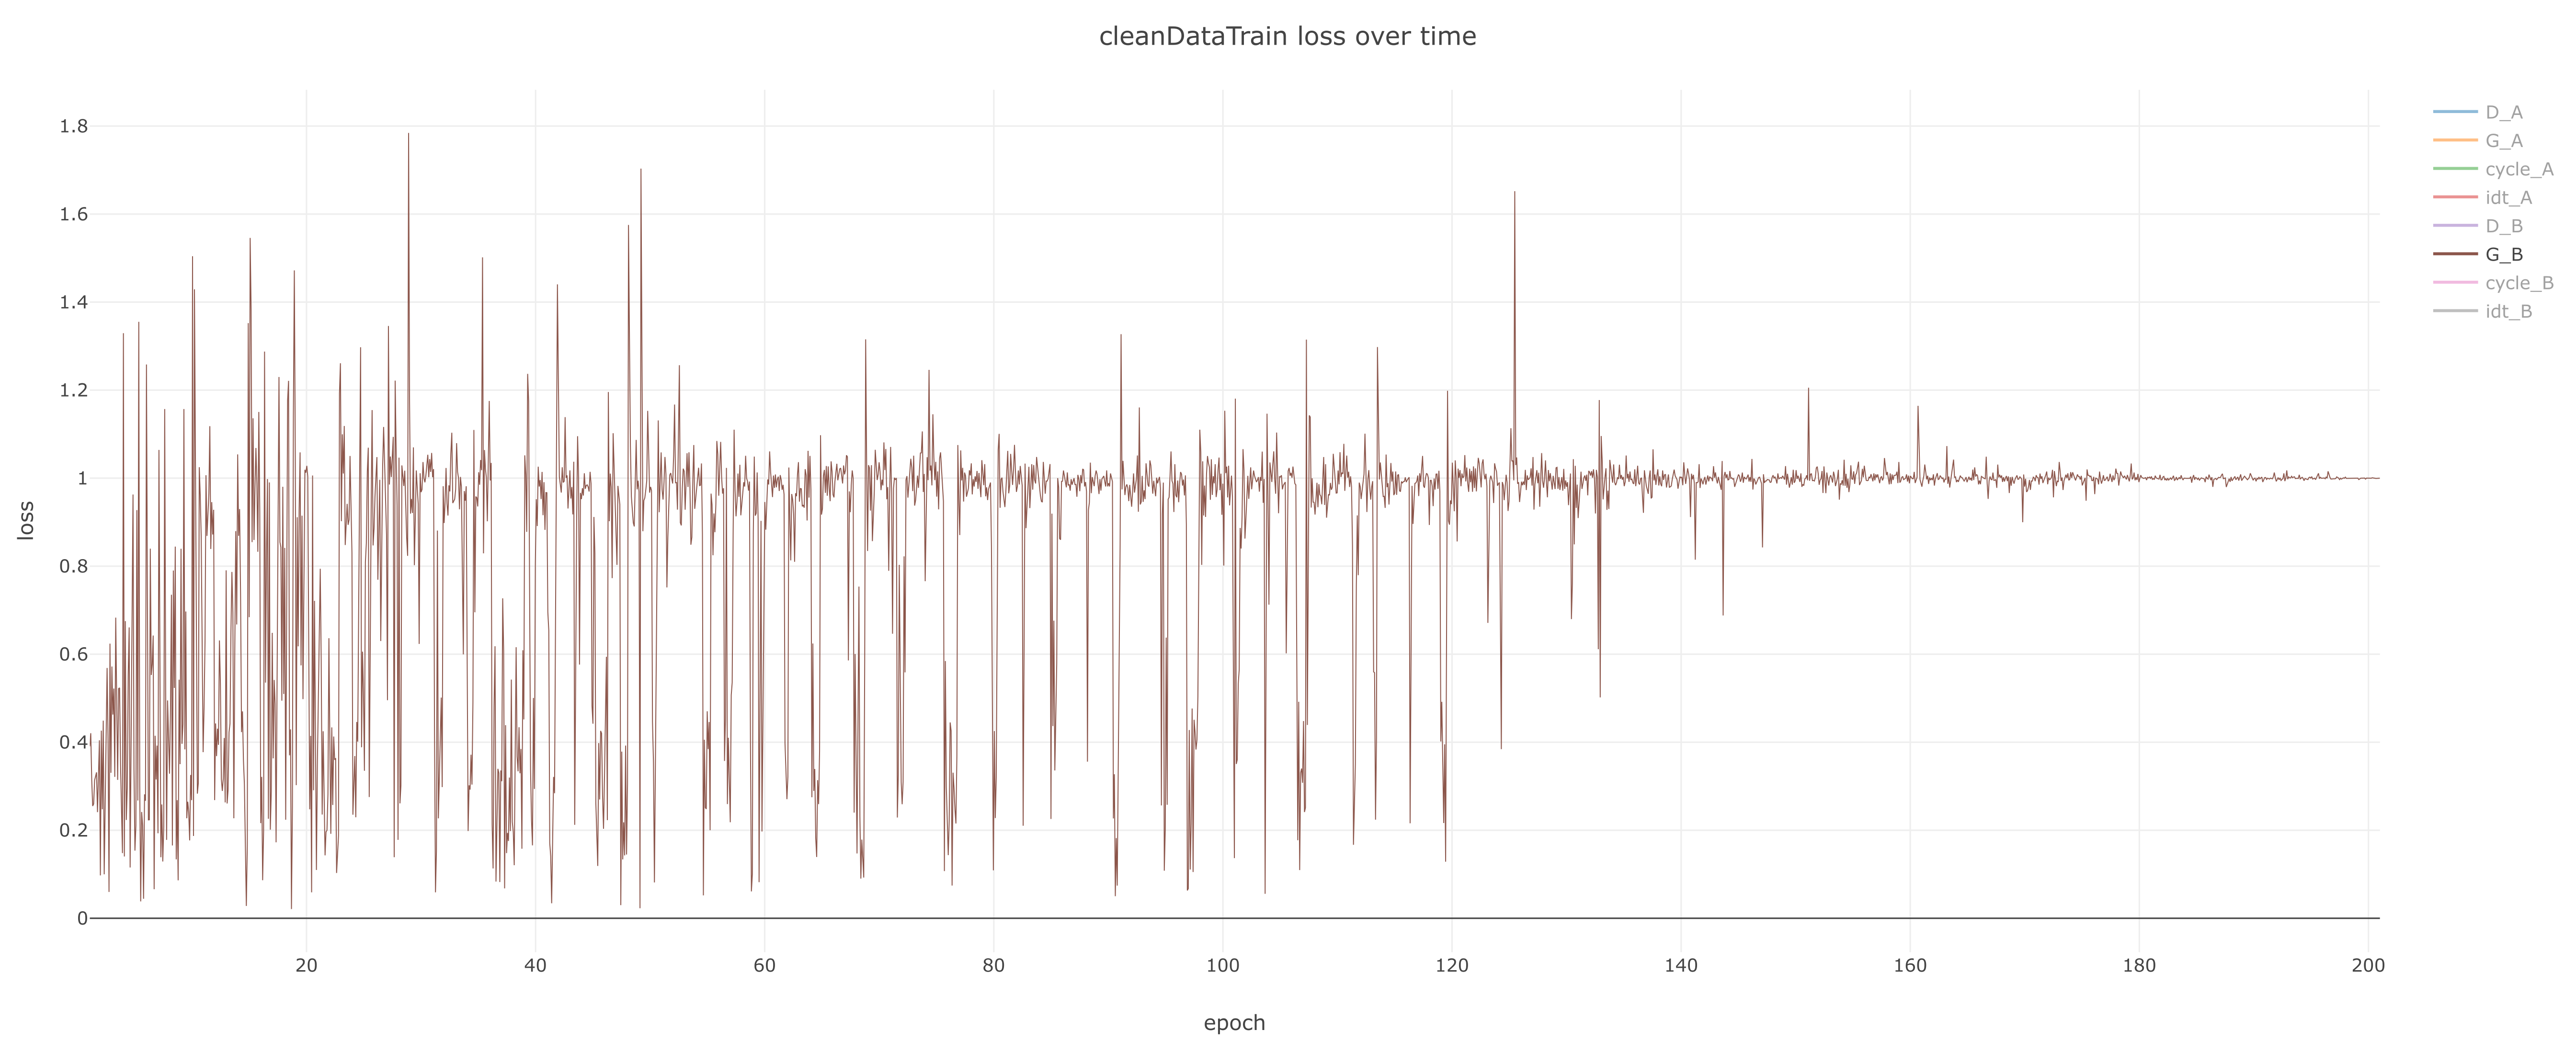
\includegraphics[width=1\textwidth]{chapter/losses_png/g_b.png}
    \caption{ Adversarial (BCE) Loss for BW Generator}
    
    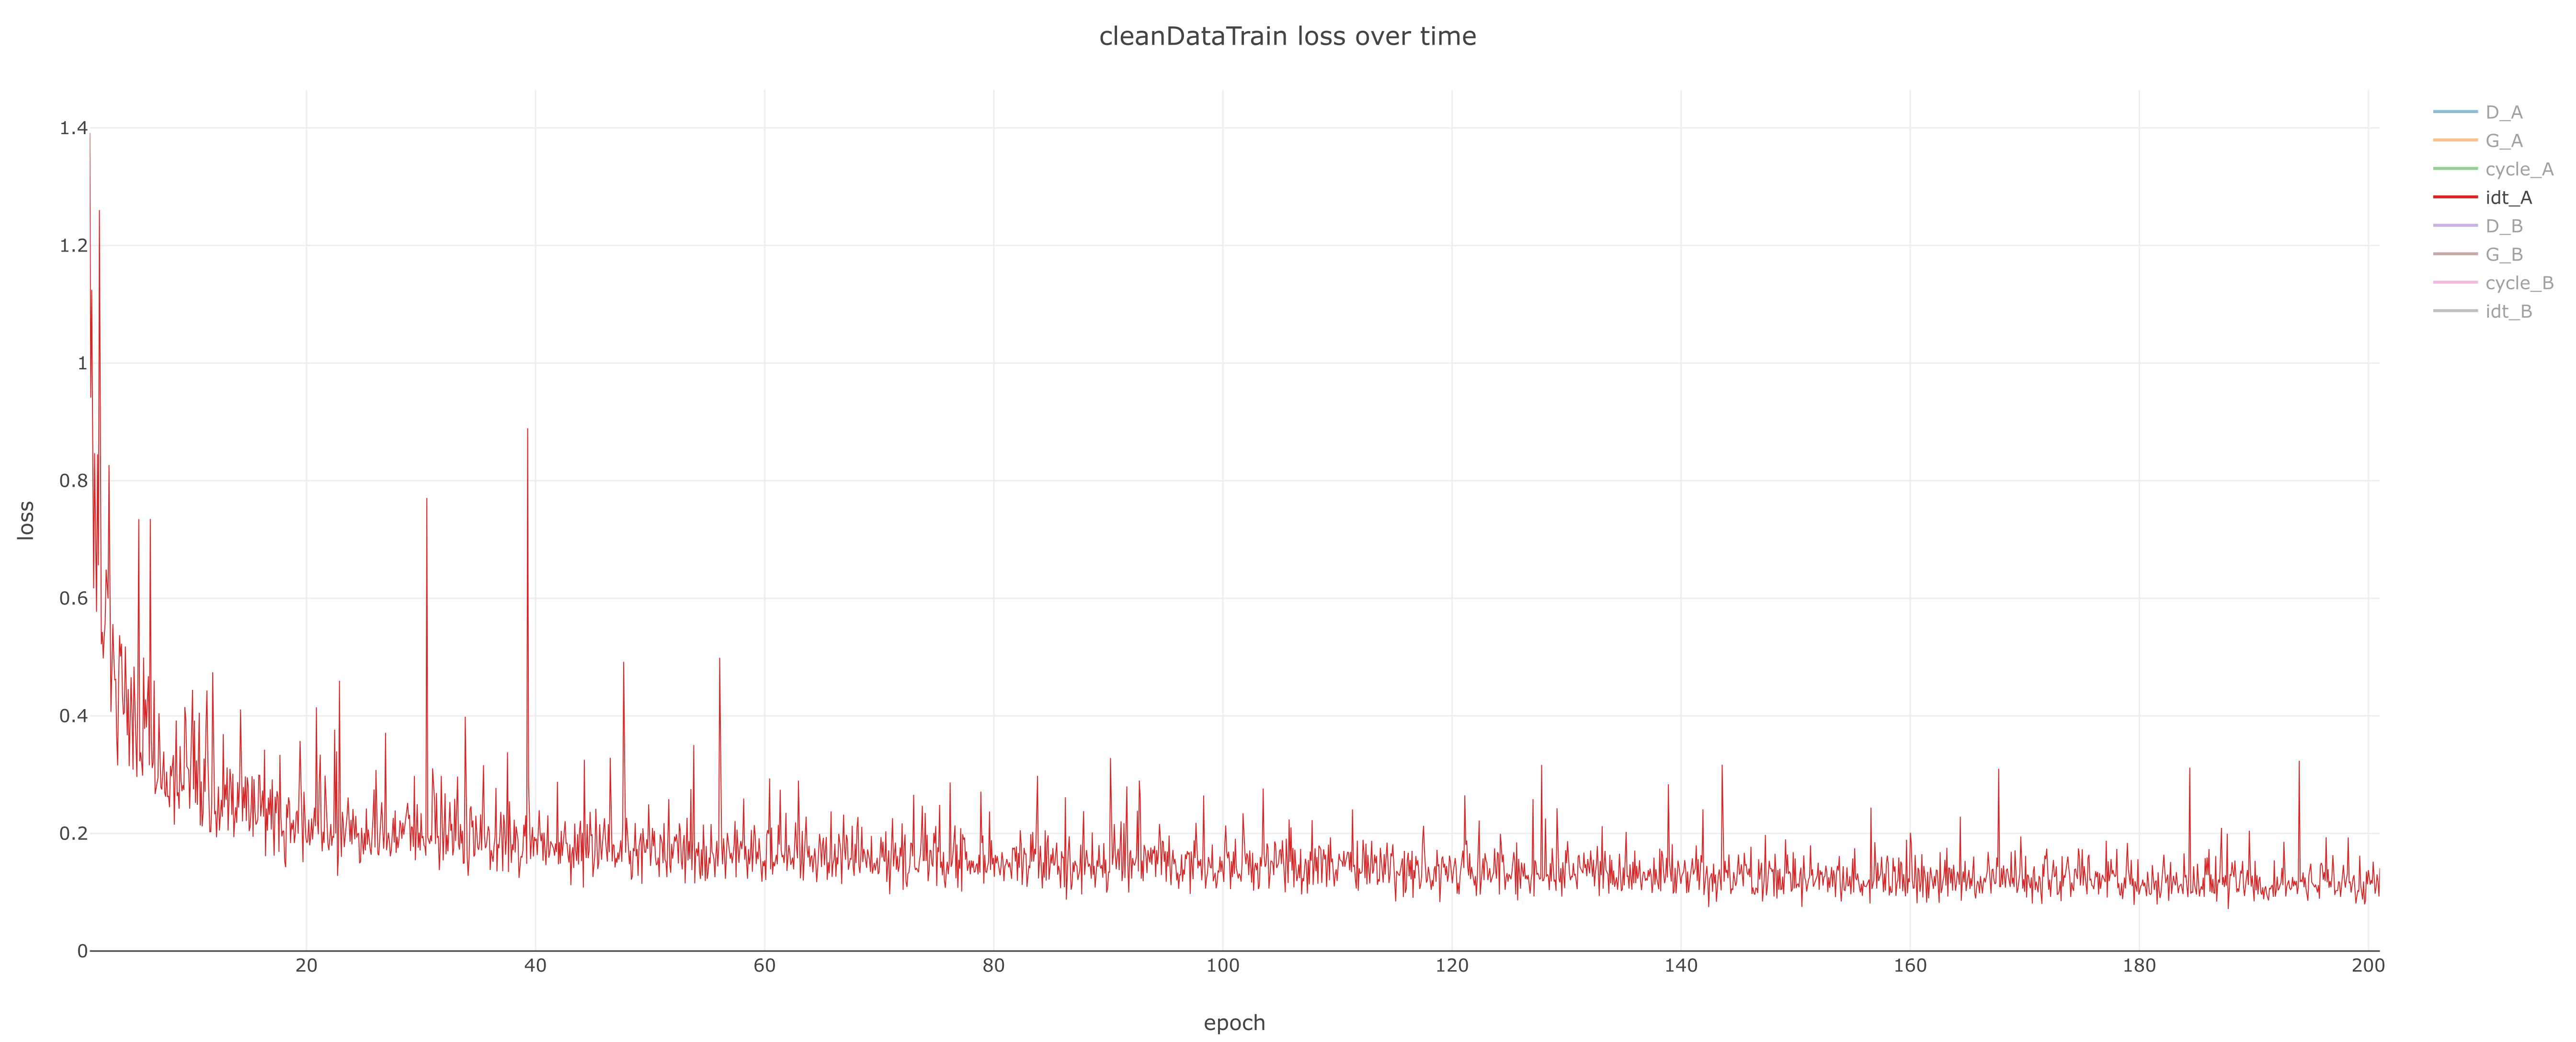
\includegraphics[width=1\textwidth]{chapter/losses_png/id_a.png}
    \caption{ Identity (L1) Loss for Color Generator}
    
    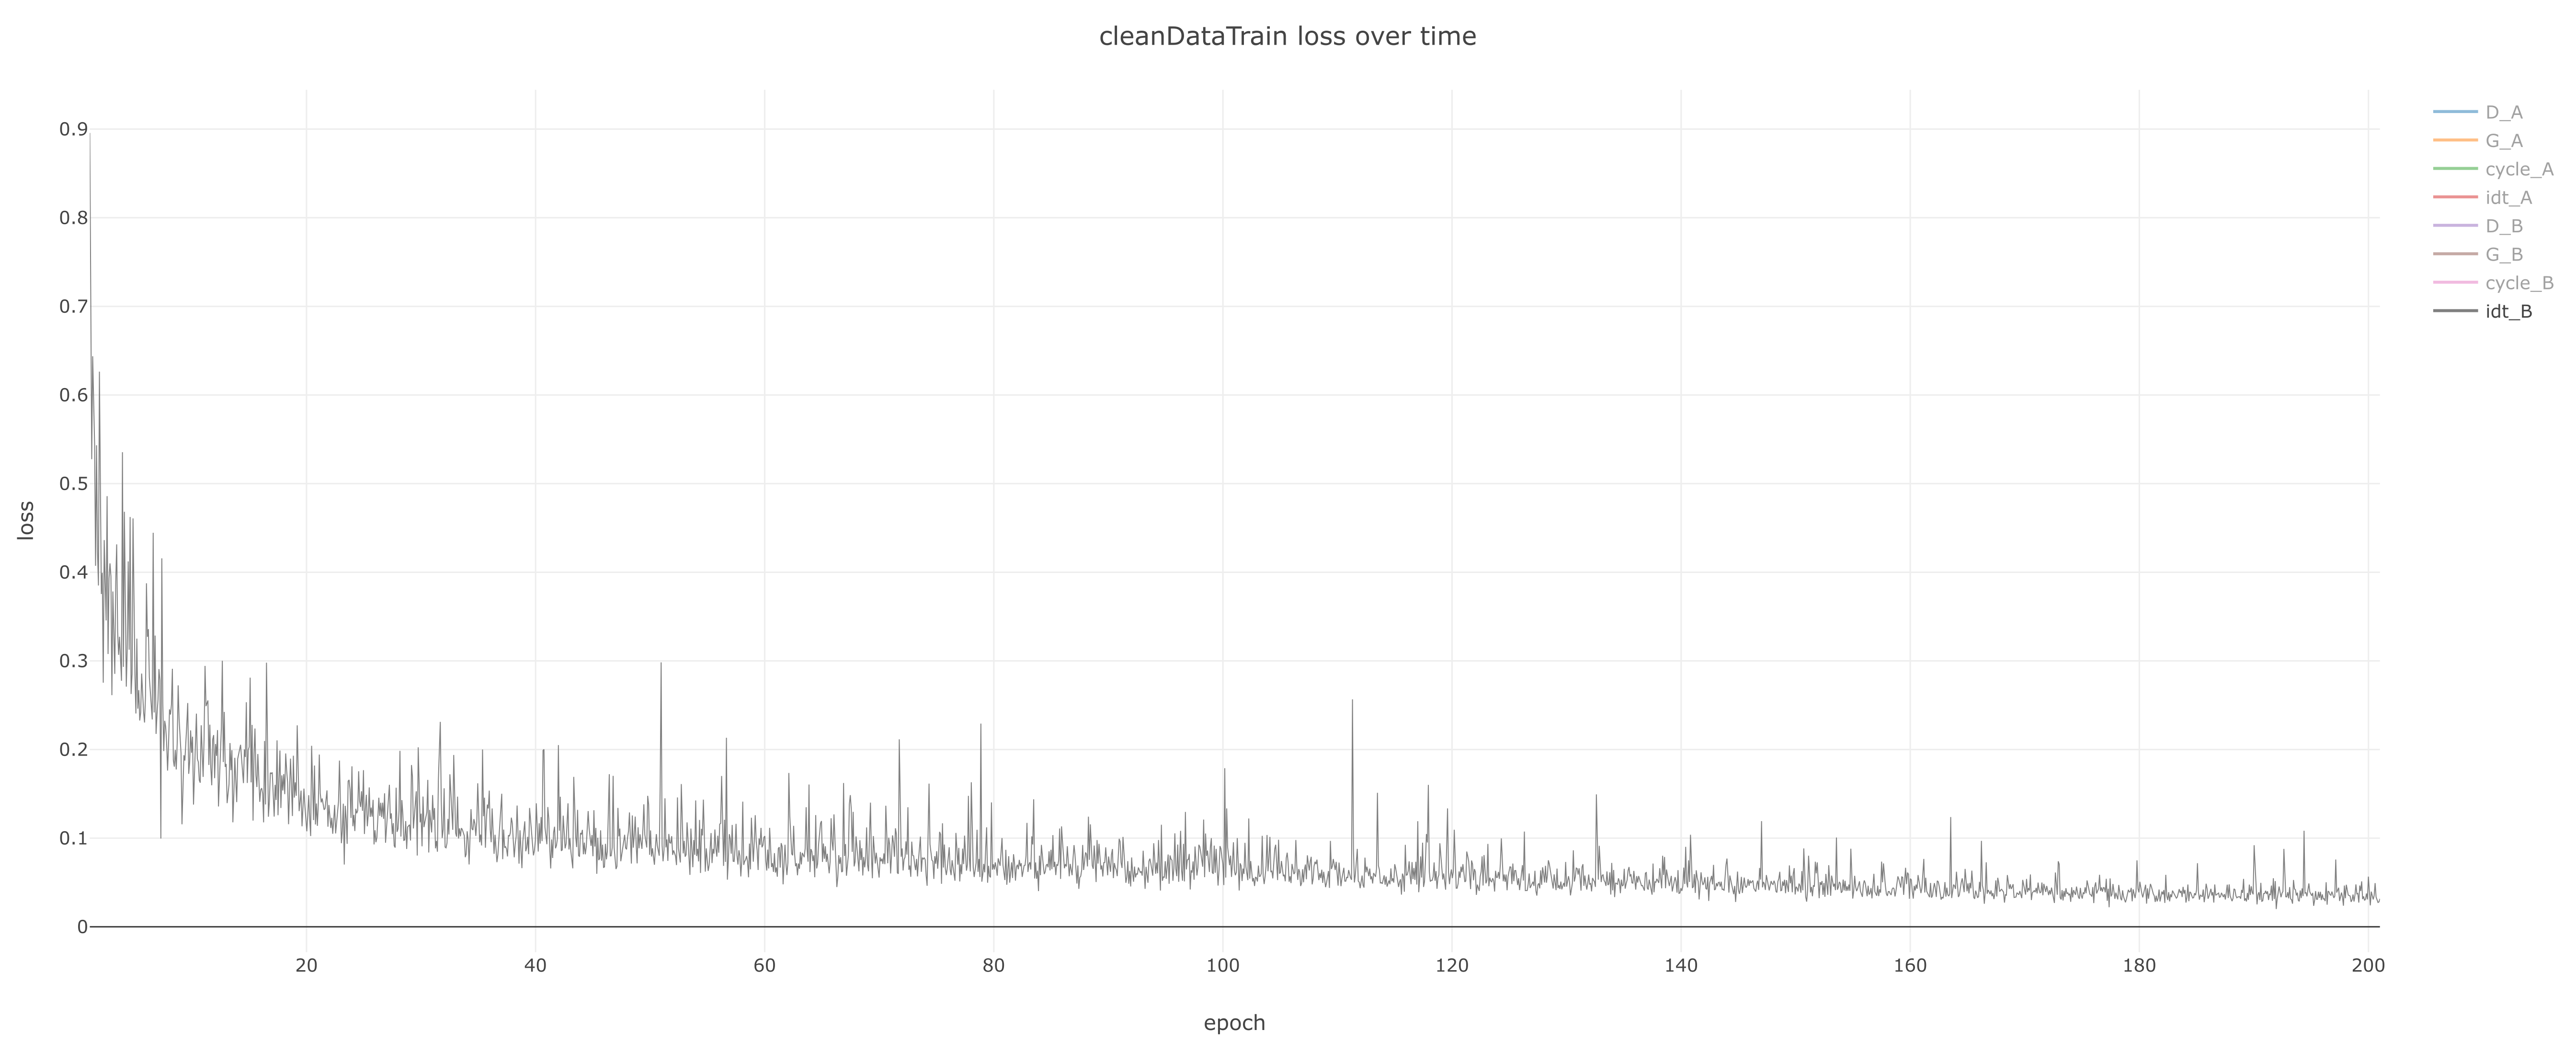
\includegraphics[width=1\textwidth]{chapter/losses_png/idt_b.png}
    \caption{ Identity (L2) Loss for Color Generator}

    \label{fig:enter-label}
\end{figure}
      \begin{itemize}
    \renewcommand\labelitemi{}
    \item   where,
    \renewcommand\labelitemi{-}
          \item   D\_A= BCE Loss for Color Discriminator, 
          \item  D\_B= BCE Loss for BW Discriminator,
          \item cycle\_A= Cycle Consistency (L1) Loss  for Color Generator, 
          \item  cycle\_B= Cycle Consistency (L1) Loss for BW Generator,
          \item  G\_A= Adversarial (BCE) Loss for Color Generator,
          \item  G\_B= Adversarial (BCE) Loss for BW Generator, 
          \item  idt\_A= Identity (L1) Loss for Color Generator,
          \item  idt\_B= Identity (L1) Loss for BW Generator
 \end{itemize}

\newpage
\subsection{Interfacing}

\subsubsection{Training Interface}
We've implemented real-time visualization of the training process and results of the model using Visdom. This integration has enhanced our ability to monitor and analyze the evolution of the model's performance at every epoch. With it, we can dynamically visualize various metrics such as loss functions, image translations, and other relevant statistics, providing us with valuable insights into the model's behavior and enabling us to make informed decisions for optimization.

\begin{figure}[h!]
  \centering
  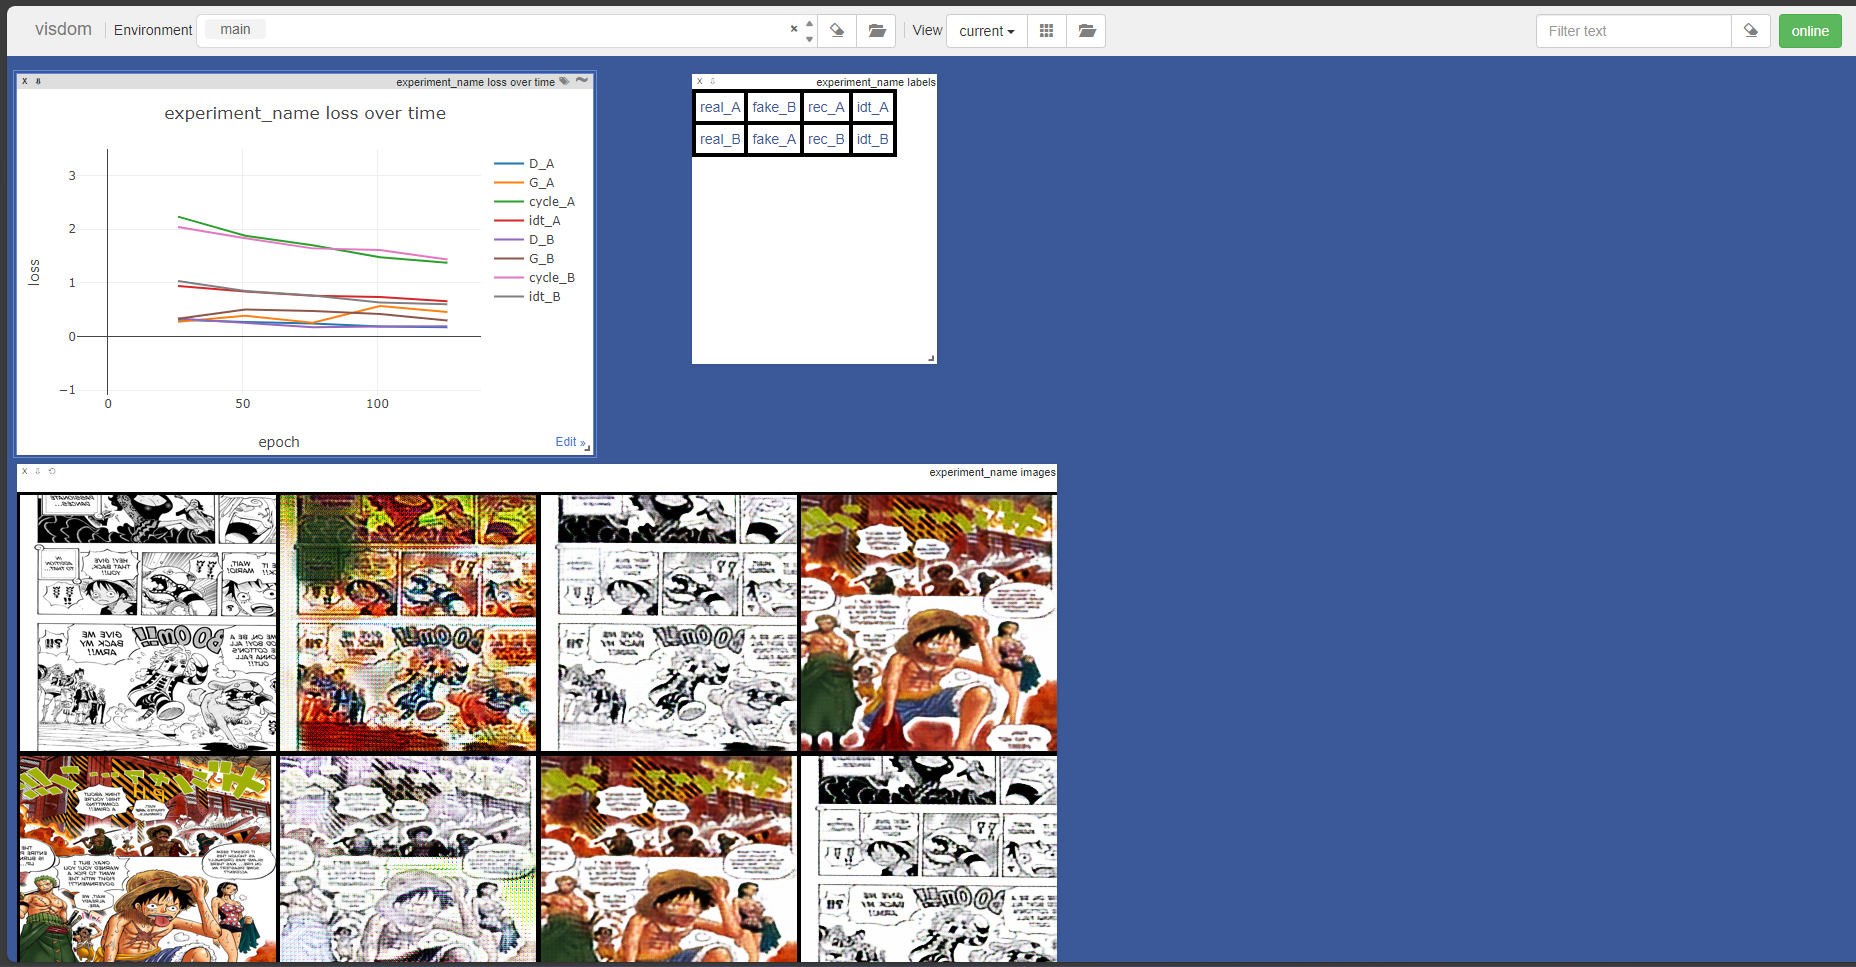
\includegraphics[width=0.8\textwidth]{img/visdom.png}
  \caption{Web-based, real-time visualization of model training and outputs}
  \label{fig:visdom}
\end{figure}

\subsubsection{User Interface}
A simple UI (figure \ref{fig:fuser_interface})has been developed using React and FastAPI for easier interaction with the model.
\begin{figure}[h!]
  \centering
  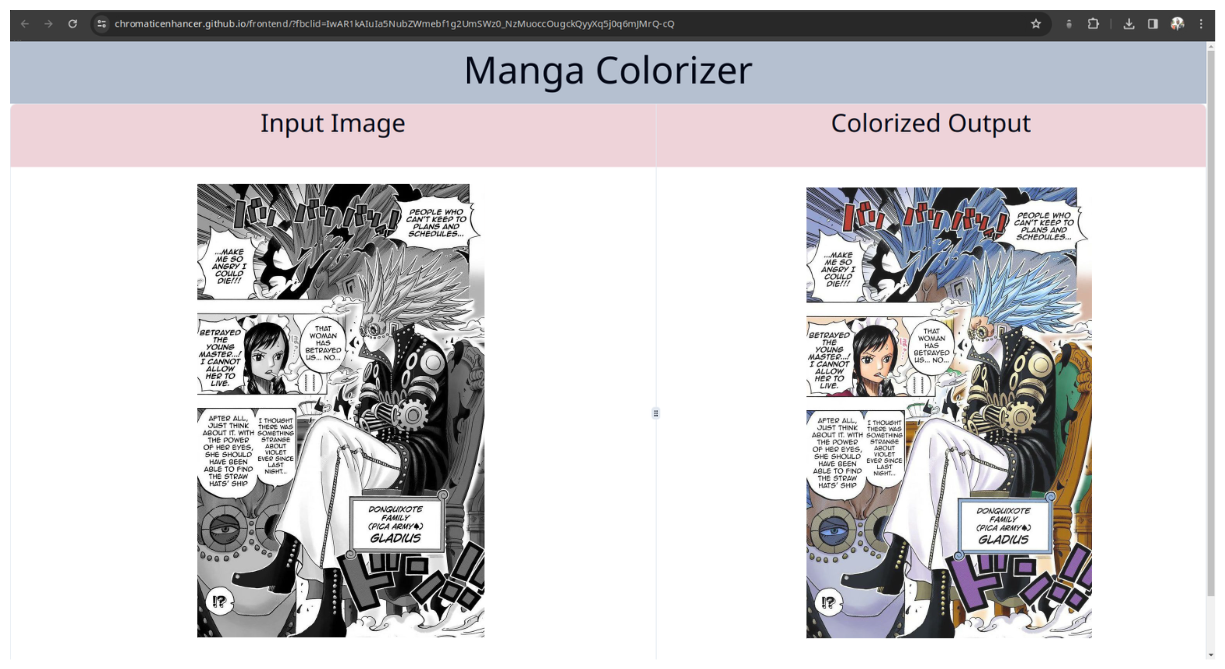
\includegraphics[width=0.8\textwidth]{img/web_interface.png}
  \caption{Demonstration of colorization via web interface}
  \label{fig:fuser_interface}
\end{figure}
    \pagenumbering{arabic}
\setcounter{page}{37}
\chapter{Expected Outcome}
The main aim of this proposed system is to streamline the process of manga colourization making it fully automatic, overcoming the shortcomings of previous colorization models and architectures such as conditional GANs\cite{10.1007/978-3-030-72610-2_17}, pix2pix\cite{isola2018imagetoimage} and style2paints\cite{ACPR2017ZLM} by reducing monotonicity and eradicating the need to provide manual color hints.\\

Ideally, our model should produce colored outputs that closely resemble those hand-painted by a human artist. However, acknowledging the complexities involved, we anticipate our model achieving results that are visually comparable to, or surpass the quality of existing semi-automatic and automatic models. It is  important to note that the subjective nature of art allows for a spectrum of color interpretations; thus, while unconventional color choices may seem unrealistic, they are not inherently incorrect. For instance, a tree painted red can still evoke artistic merit within a specific style or context. \\

Given this consideration, it's crucial to recognize that the absence of contextual understanding within the text could lead to unintended outcomes. For instance, in a scenario where a manga text describes a "bright green bird," the model might erroneously color the bird white if it lacks contextual awareness and hasn't been exposed to a diverse range of bird illustrations in its training dataset.

\begin{figure}[htbp]
    \centering
    \begin{subfigure}[b]{0.48\textwidth}
        \includegraphics[width=\textwidth]{img/expected_bw.png}
        \caption{Black and white manga cover}
      
    \end{subfigure}
    \hfill
    \begin{subfigure}[b]{0.48\textwidth}
        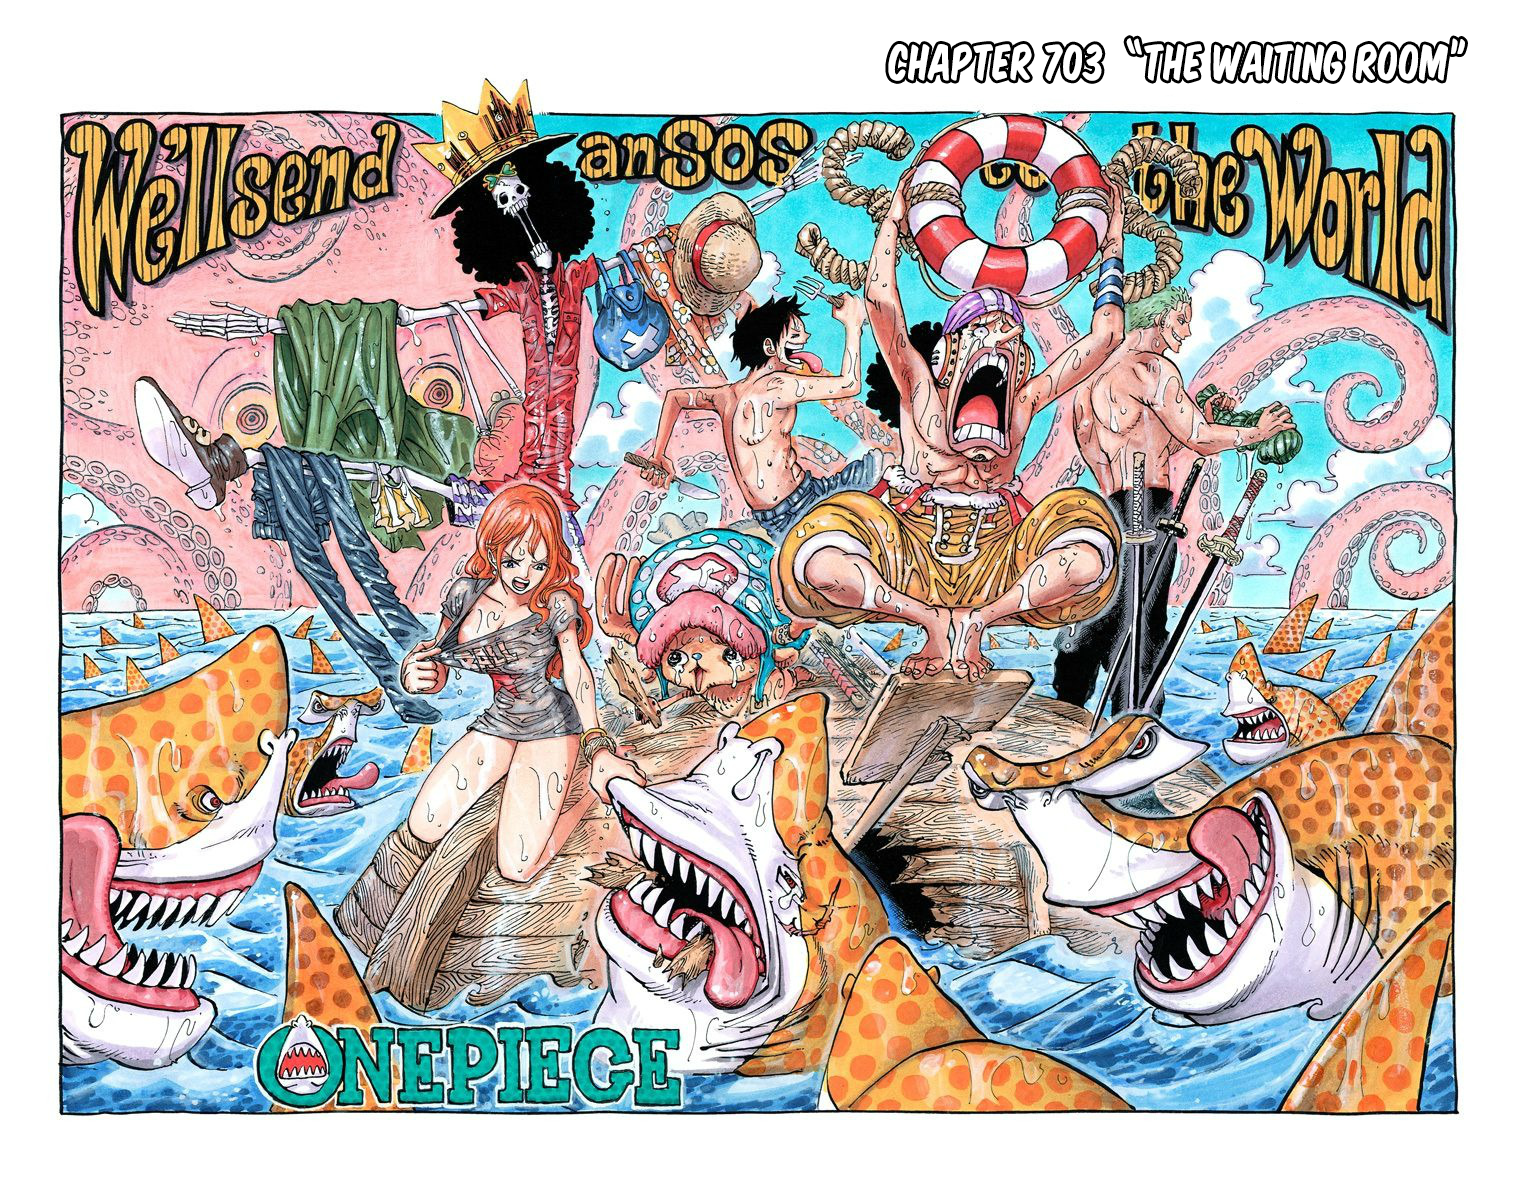
\includegraphics[width=\textwidth]{img/expected_human-drawn_ideal.png}
        \caption{human-colored manga cover}

    \end{subfigure}
    
\caption{Expected outcome for ideal automatic colorizer}
\label{fig:bad_images}
    
\end{figure}
\pagebreak
    
\chapter{Actual Outcomes}

\pagenumbering{arabic}
\setcounter{page}{38}

% losses highlight 

\section{GAN losses (200 epochs)}

\begin{table}[h]
    \centering
    \begin{tabular}{|l|l|} \hline 
        Discriminator\_A & 0.083 \\ \hline 
        Generator\_A & 0.613 \\ \hline 
        Cycle\_A & 0.298 \\ \hline 
        Identity\_A & 0.141 \\ \hline 
        Discriminator\_B & 0.000 \\ \hline 
        Generator\_B & 1.000 \\ \hline 
        Cycle\_B & 0.299 \\ \hline 
        Identity\_B & 0.032 \\ \hline
        
    \end{tabular}
    
    \caption{Losses on training for 200 epochs}
    \label{table:table_loss}
   
   \noindent where,\\
    A = Black and White Dataset\\
    B= Colored Dataset \\
\end{table}
     
\noindent The losses for Generators and Discriminators reached the values as in \ref{table:table_loss} at the end of 200th epoch. The discriminator for colored image had its loss converged to 0 while the loss of the generator peaked to 1.  The effect of adversarial nature of the networks was seen in the graph of losses. Color generator and color discriminator losses reached plateau at around 160 epochs.

\clearpage
\section{Test Results (different sized inputs)}
% test results


\begin{figure}[h!]
  \centering
  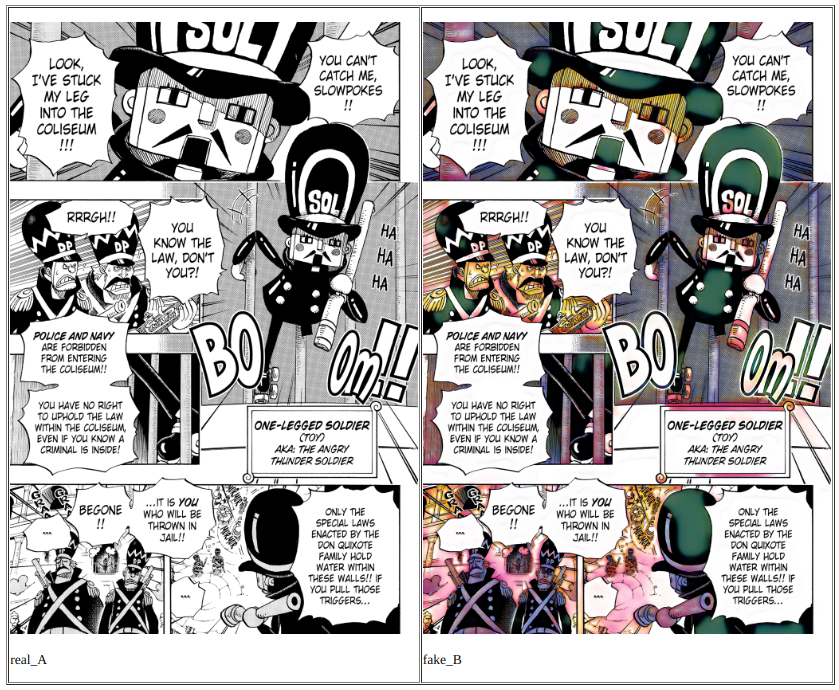
\includegraphics[width=0.8\textwidth]{chapter/actual/acx.png}
 
  \label{fig:final UI}
\end{figure}
\begin{figure}[h!]
  \centering
  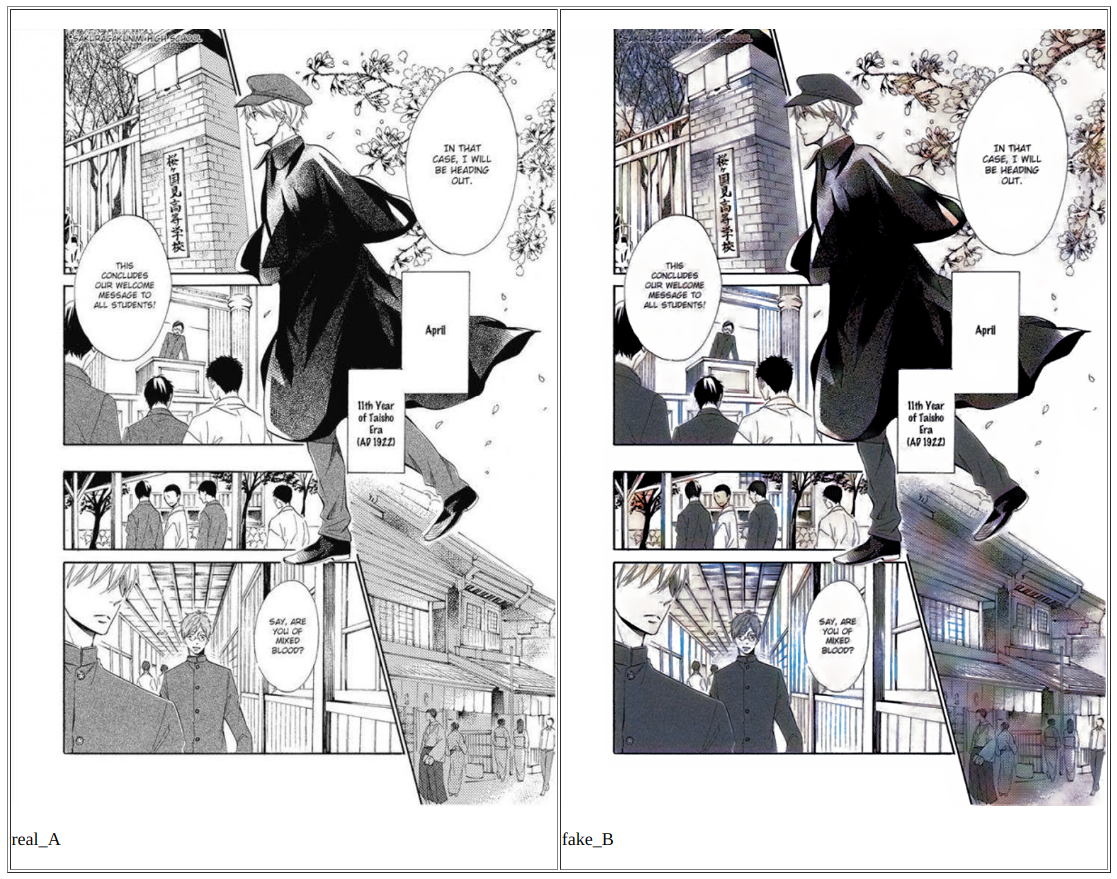
\includegraphics[width=0.8\textwidth]{chapter/actual/acu.png}
  \label{fig:final UI}
\end{figure}
\newpage
\begin{figure}[h!]
  \centering
  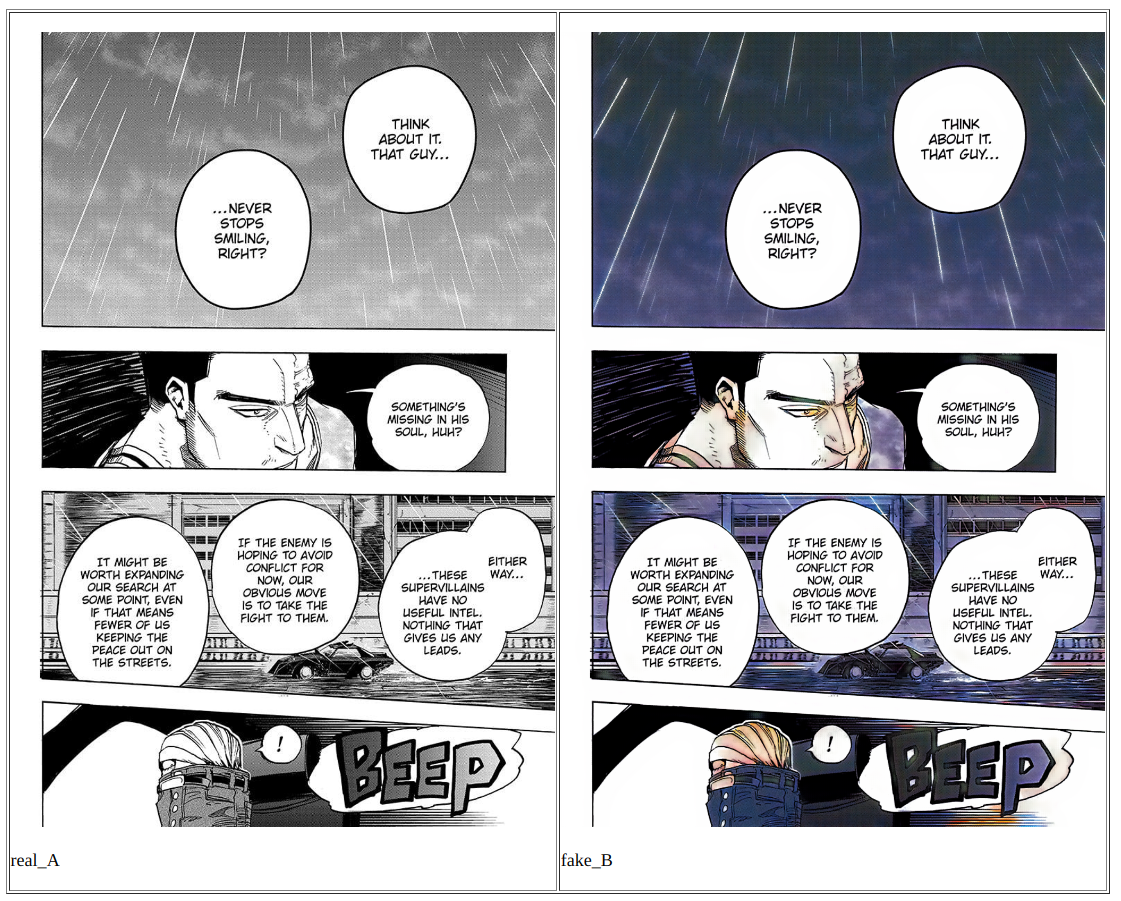
\includegraphics[width=0.8\textwidth]{chapter/actual/acy.png}
  \label{fig:final UI}
\end{figure}
\begin{figure}[h!]
  \centering
  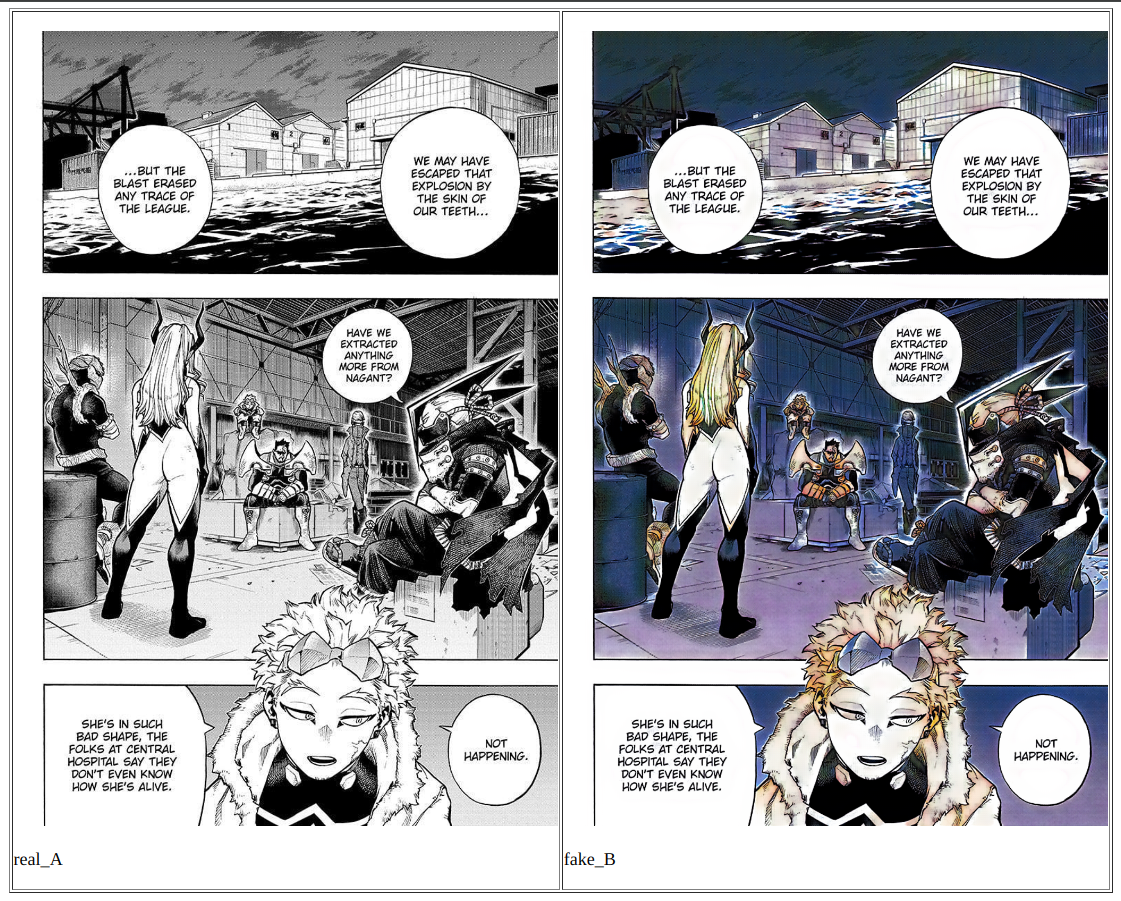
\includegraphics[width=0.8\textwidth]{chapter/actual/acz.png}
  \label{fig:final UI}
\end{figure}

For testing and deployment, we only need to load the color generator. So far, it's been impressively consistent with colors across panels on a page, especially in darker and shaded spots where it fills in suitable colors that match the environment's mood. It made sure to steer clear of coloring over text blobs, and inherently white backgrounds.The details in reconstructed image remain intact and the test is well-readable. Despite being trained on cropped images from a small dataset, it's adapting well to a range of new test images. Our model can handle high-definition images of different sizes and colorize them effectively.
% describe kk xa, similar color of hair can be seen, ani text ni high res, text blobs uncolored, any size of input can be given, 256x256 ma train garyo bhane the closer the test input is to 256x256, the better is the op. ani crop garera, resize nagari train garyo bhane, larger test inputs ma better results. 
\clearpage
%limitation
\subsection{Limitations}
While our model excels at coloring manga panels at certain scenarios such as dark room or rainy/cloudy weather, it fails to produce such good results at other scenarios. It also seems to have heavy inclination towards blue color. 

\begin{figure}[hbtp]
    \centering
    \begin{subfigure}[b]{0.48\textwidth}
        \includegraphics[width=\textwidth]{chapter/actual/ac3.png}
    \end{subfigure}
    \hfill
    \begin{subfigure}[b]{0.45\textwidth}
        \includegraphics[width=\textwidth]{chapter/actual/ac1.png}
    \end{subfigure}
    \caption{Failed colorized outputs}
        \label{fig:bad_images}
\end{figure}


\section{Performance Evaluation}
% performance evaluation
In evaluating the fidelity of the reconstructed images compared to their original counterparts, we utilized Peak Signal-to-Noise Ratio (PSNR) as a metric. This measure allows for a quantitative evaluation of reconstruction quality, with higher PSNR values indicating higher fidelity. Our assessment involved four different images, each representative of distinct manga panel styles. Across all image pairs, the PSNR values were consistently high, averaging at 24.3742 dB. This average PSNR suggests satisfactory performance of the color generator in reconstructing the images.

To evaluate structural similarity between the original and reconstructed images, we employed the Structural Similarity Index (SSIM). SSIM considers various aspects such as luminance, contrast, and structure, providing a comprehensive assessment. SSIM values range from -1 to 1, with 1 indicating perfect similarity. While slight visual differences were observed between the image pairs, the average SSIM value of 0.9039 confirms that the reconstructed images maintain structural coherence.

In summary, our CycleGAN model has demonstrated reasonable performance based on both PSNR and SSIM scores, indicating successful image reconstruction. Nonetheless, further optimization through fine-tuning or experimentation, along with training on a larger dataset, may yield even more desirable results.


\begin{figure} [htbp]
    \centering
        \includegraphics[height=0.4\textwidth]{img_psnr/perf_metrics.jpg}
    \caption{Real(top row) and Reconstructed colored (bottom row) images}
    \label{fig:comparision real and reconstructed}
\end{figure}


\begin{table} [htbp]
    \centering
    \begin{tabular}{|c|c|c|} \hline
         Image Pair Labels&  PSNR&  SSIM\\ \hline 
            a&  24.5019&  0.9404\\ \hline 
            b&  24.2575&  0.8277\\ \hline
            c& 24.8711& 0.9297\\\hline
            d& 23.8663& 0.9180\\\hline
            Average& 24.3742& 0.9039\\\hline
    \end{tabular}
    \label{tab:PSNR and SSIM table for real and reconstructed real images }
    \caption{PSNR and SSIM table for real and reconstructed real images }
\end{table}

    \chapter{Conclusion and Future Enhancements}

Conclusively, for the project Automatic Colorization of Japanese Comics using GANs is completed as it was successfully deployed as a python package and a website.
\\
As per future enhancements following can be considered:
    \begin{itemize}
        \item Use of  contrastive-unpaired-translation to reduce the time and resources required for training\cite{park2020contrastive}
        \item Better hardware can be used to train image in higher resolution to get more quality results
        \item Better and larger datasets can be used to accomodate colorization of variety of scenarios
    \end{itemize}
    \bibliographystyle{IEEEtran}
    \bibliography{ref}
	\addcontentsline{toc}{chapter}{Bibliography}
    \renewcommand{\thesection}{\Alph{section}}
\end{document}